%-----------------------------------------------
%  Engineer's & Master's Thesis Template
%  Copyleft by Artur M. Brodzki & Piotr Woźniak
%  Warsaw University of Technology, 2019-2022
%-----------------------------------------------

\documentclass[
    bindingoffset=5mm,  % Binding offset
    footnoteindent=3mm, % Footnote indent
    hyphenation=true    % Hyphenation turn on/off
]{src/wut-thesis}

\graphicspath{{tex/img/}} % Katalog z obrazkami.
\addbibresource{bibliografia.bib} % Plik .bib z bibliografią
\raggedbottom

%-------------------------------------------------------------
% Wybór wydziału:
%  \facultyeiti: Wydział Elektroniki i Technik Informacyjnych
%  \facultymeil: Wydział Mechaniczny Energetyki i Lotnictwa
% --
% Rodzaj pracy: \EngineerThesis, \MasterThesis
% --
% Wybór języka: \langpol, \langeng
%-------------------------------------------------------------
\facultyeiti    % Wydział Elektroniki i Technik Informacyjnych
\MasterThesis % Praca magisterska
\langpol % Praca w języku polskim

\begin{document}

%------------------
% Strona tytułowa
%------------------
\instytut{Telekomunikacji}
\kierunek{Telekomunikacja}
\specjalnosc{Teleinformatyka i cyberbezpieczeństwo}
\title{
    Badanie efektywności uczenia ze wzmocnieniem w adaptacyjnym sterowaniu ruchem drogowym
}

\engtitle{
    A Study on the Effectiveness of Reinforcement Learning in Adaptive Traffic Control
}
\author{Tomasz Lewiński}
\album{323692}
\promotor{dr inż Tomasz Mrozek}
\date{\the\year}
\maketitle

%-------------------------------------
% Streszczenie po polsku dla \langpol
% English abstract if \langeng is set
%-------------------------------------
\cleardoublepage % Zaczynamy od nieparzystej strony
\abstract

\keywords

%----------------------------------------
% Streszczenie po angielsku dla \langpol
% Polish abstract if \langeng is set
%----------------------------------------
\clearpage
\secondabstract

\secondkeywords

\pagestyle{plain}

%--------------
% Spis treści
%--------------
\cleardoublepage % Zaczynamy od nieparzystej strony
\tableofcontents

%------------
% Rozdziały
%------------
\cleardoublepage % Zaczynamy od nieparzystej strony
\pagestyle{headings}

\clearpage
\section*{Przedmowa}

Odkąd jeżdżę samochodem po Warszawie, zastanawiam się, jak faktycznie działa sygnalizacja świetlna. Na drogach wielokrotnie spotykałem się z sytuacjami, w których wydawało mi się, że sygnalizacja działa w sposób nieoptymalny. Jest to problem, który do dzisiaj nie daje mi spokoju.

Dlatego kiedy na studiach zainteresowałem się uczeniem maszynowym, zacząłem się zastanawiać, czy nie można by wykorzystać modeli uczenia ze wzmocnieniem właśnie do optymalizacji ruchu drogowego. Wydaje mi się, że jest to technologia z dużym potencjałem w tym zastosowaniu, ponieważ algorytm uczy się dostosowywać swoją politykę do konkretnego skrzyżowania. Nie są potrzebne ręcznie oznaczone zbiory treningowe, potrzebne są natomiast metoda obserwacji środowiska, możliwość podejmowania w nim akcji oraz funkcja nagrody.

Ponieważ kończę już studia na tym kierunku, chciałbym w tym miejscu podziękować moim kolegom i koleżankom za przejście tej drogi razem ze mną, wspólne projekty, naukę do kolokwiów i wzajemne motywowanie się do ukończenia studiów oraz kontynuowania nauki na studiach magisterskich. Bez Was na pewno byłoby dużo trudniej i nie byłaby to taka dobra zabawa.

\clearpage
\section{Wstęp}
\label{sec:wstep}

\subsection{Wprowadzenie do problematyki}
\label{subsec:wprowadzenie}

Zatory drogowe wydłużają czas przejazdu, a związany z nimi ruch z częstym zatrzymywaniem i ruszaniem zwiększa zużycie paliwa oraz emisję zanieczyszczeń \cite{treiber2008congestion}.

Jednym z podstawowych narzędzi zarządzania ruchem w miastach jest sterowanie sygnalizacją świetlną na skrzyżowaniach. Sposób przydzielania prawa przejazdu poszczególnym strumieniom pojazdów bezpośrednio wpływa na przepustowość skrzyżowania, czas oczekiwania oraz długość kolejek, a tym samym na sprawność całej sieci drogowej \cite{LEITNER2022507}.

Tradycyjne programy sygnalizacji często działają według z góry ustalonych reguł. W sterowaniu stałoczasowym sekwencję faz i czas ich trwania określa się z góry, bez uwzględniania bieżącej sytuacji ruchowej. Bardziej zaawansowane metody, takie jak sterowanie akomodacyjne typu gap-based, reagują na obecność i napływ pojazdów, ale nadal opierają się na ustalonej logice, a nie na polityce wyuczonej na podstawie doświadczenia.

Alternatywą jest adaptacyjne sterowanie wykorzystujące uczenie ze wzmocnieniem. Agent uczy się polityki przez interakcję ze środowiskiem: obserwuje stan skrzyżowania, wybiera fazę sygnalizacji i otrzymuje nagrodę oceniającą skutki tej decyzji. Polityka nie musi więc być z góry zaprogramowana, ponieważ powstaje podczas uczenia. Potencjał tego podejścia jest punktem wyjścia pracy.

\subsection{Problem badawczy i hipoteza}
\label{subsec:problem-hipoteza}

Sformułowano następujące pytanie badawcze:
\begin{quote}
    \emph{Czy algorytm głębokiego uczenia ze wzmocnieniem może sterować sygnalizacją świetlną na pojedynczym skrzyżowaniu skuteczniej niż sterowanie stałoczasowe oraz akomodacyjne?}
\end{quote}

Przyjęto również następującą hipotezę:
\begin{quote}
    \emph{Odpowiednio wytrenowany algorytm DQN może zmniejszyć opóźnienie, czas oczekiwania oraz długość kolejek pojazdów względem klasycznych metod sterowania, szczególnie w warunkach zmiennego lub wysokiego natężenia ruchu.}
\end{quote}

Hipoteza dotyczy wskaźników opisujących płynność ruchu, przede wszystkim opóźnienia, czasu oczekiwania oraz długości kolejek. Ich poprawa nie musi jednak oznaczać przewagi DQN według każdej metryki ani w każdym scenariuszu. Może się na przykład wiązać z częstszym przełączaniem sygnalizacji. Zakres i warunki potwierdzenia hipotezy oceniono w dalszej części pracy, porównując metody sterowania na odrębnym zbiorze testowym.

\subsection{Cel i zakres pracy}
\label{subsec:cel-zakres}

Celem pracy jest zaprojektowanie, wytrenowanie oraz ocena algorytmu DQN sterującego sygnalizacją świetlną na zamodelowanym skrzyżowaniu ulicy Belgradzkiej i alei Komisji Edukacji Narodowej (al. KEN).

Aby osiągnąć ten cel, zrealizowano następujące cele szczegółowe:
\begin{itemize}
    \item odwzorowanie skrzyżowania w środowisku symulacyjnym SUMO;
    \item implementacja środowiska uczenia ze wzmocnieniem, integrującego symulację z procesem treningowym;
    \item zdefiniowanie przestrzeni obserwacji, przestrzeni akcji oraz funkcji nagrody;
    \item przygotowanie rozdzielnych zbiorów: treningowego, walidacyjnego oraz testowego;
    \item implementacja metod referencyjnych: sterowania stałoczasowego oraz akomodacyjnego;
    \item wyznaczenie odpowiedniej liczby kroków treningowych;
    \item porównanie dwóch sposobów generowania danych treningowych;
    \item dobór hiperparametrów algorytmu DQN;
    \item ocena stabilności procesu uczenia;
    \item porównanie rozpatrywanych metod na odrębnym zbiorze testowym.
\end{itemize}

\subsection{Założenia i ograniczenia pracy}
\label{subsec:zalozenia-ograniczenia}

Zakres pracy świadomie ograniczono, aby przeprowadzić kontrolowany eksperyment. Badano pojedyncze skrzyżowanie bez uwzględniania wpływu skrzyżowań sąsiednich. W modelu ruchu uwzględniono wyłącznie pojazdy silnikowe, pomijając ruch pieszy, rowerowy i komunikację miejską. Ruch drogowy wygenerowano syntetycznie za pomocą skryptu \texttt{randomTrips.py} \cite{sumo_randomtrips_docs}, dlatego nie odwzorowuje on bezpośrednio rzeczywistych pomiarów natężenia. Wszystkie eksperymenty przeprowadzono wyłącznie w symulacji, bez wdrożenia na rzeczywistym sterowniku sygnalizacji.

Celem pracy nie było stworzenie gotowego systemu produkcyjnego ani certyfikowanego sterownika ruchu. Przeprowadzono kontrolowany eksperyment, aby ocenić potencjał DQN w adaptacyjnym sterowaniu sygnalizacją świetlną w porównaniu z klasycznymi, deterministycznymi metodami sterowania.

\clearpage
\section{Przegląd metod sterowania ruchem i istniejących rozwiązań}

\clearpage
\section{Metodyka badań i opracowanie algorytmu sterowania}
\label{sec:metodyka}

\subsection{Koncepcja eksperymentu}
\label{subsec:koncepcja}

Badanie zaprojektowano jako kontrolowany eksperyment porównawczy, w którym agent uczony metodą uczenia ze wzmocnieniem oraz dwie klasyczne metody referencyjne sterują tą samą siecią drogową i są oceniane na tych samych scenariuszach ruchu. Nadrzędnym założeniem metodycznym było oddzielenie danych wykorzystywanych do uczenia i strojenia modelu od danych służących do końcowej oceny.

Procedurę badawczą podzielono na następujące etapy:
\begin{enumerate}
    \item przygotowanie modelu skrzyżowania w środowisku symulacyjnym SUMO;
    \item wygenerowanie scenariuszy ruchu odpowiadających różnym poziomom natężenia;
    \item podział danych na zbiór treningowy, walidacyjny i testowy;
    \item dobór parametrów czasowych metod referencyjnych na podstawie scenariuszy treningowych;
    \item trening modeli DQN na przygotowanych danych treningowych;
    \item wyznaczenie odpowiedniej liczby kroków treningowych oraz porównanie dwóch sposobów generowania danych treningowych;
    \item dobór hiperparametrów metodą zmiany pojedynczego parametru;
    \item zamrożenie wybranej konfiguracji jako modelu końcowego;
    \item końcowa ocena modelu na odrębnym zbiorze testowym;
    \item porównanie wyników agenta DQN z wynikami metod klasycznych.
\end{enumerate}

Wybór i strojenie modelu DQN oraz dobór parametrów metod referencyjnych realizowano wyłącznie na danych treningowych i walidacyjnych. Zbiór testowy służył do porównania zamrożonych konfiguracji metod i nie stanowił formalnego kryterium wyboru DQN. Chronologię jego wykorzystania oraz wynikające z niej ograniczenie omówiono w podrozdziale~\ref{subsec:ograniczenia-wiarygodnosci}. Schemat całego procesu badawczego przedstawiono na rysunku~\ref{fig:proces-badawczy}.

\begin{figure}[!htbp]
    \centering
    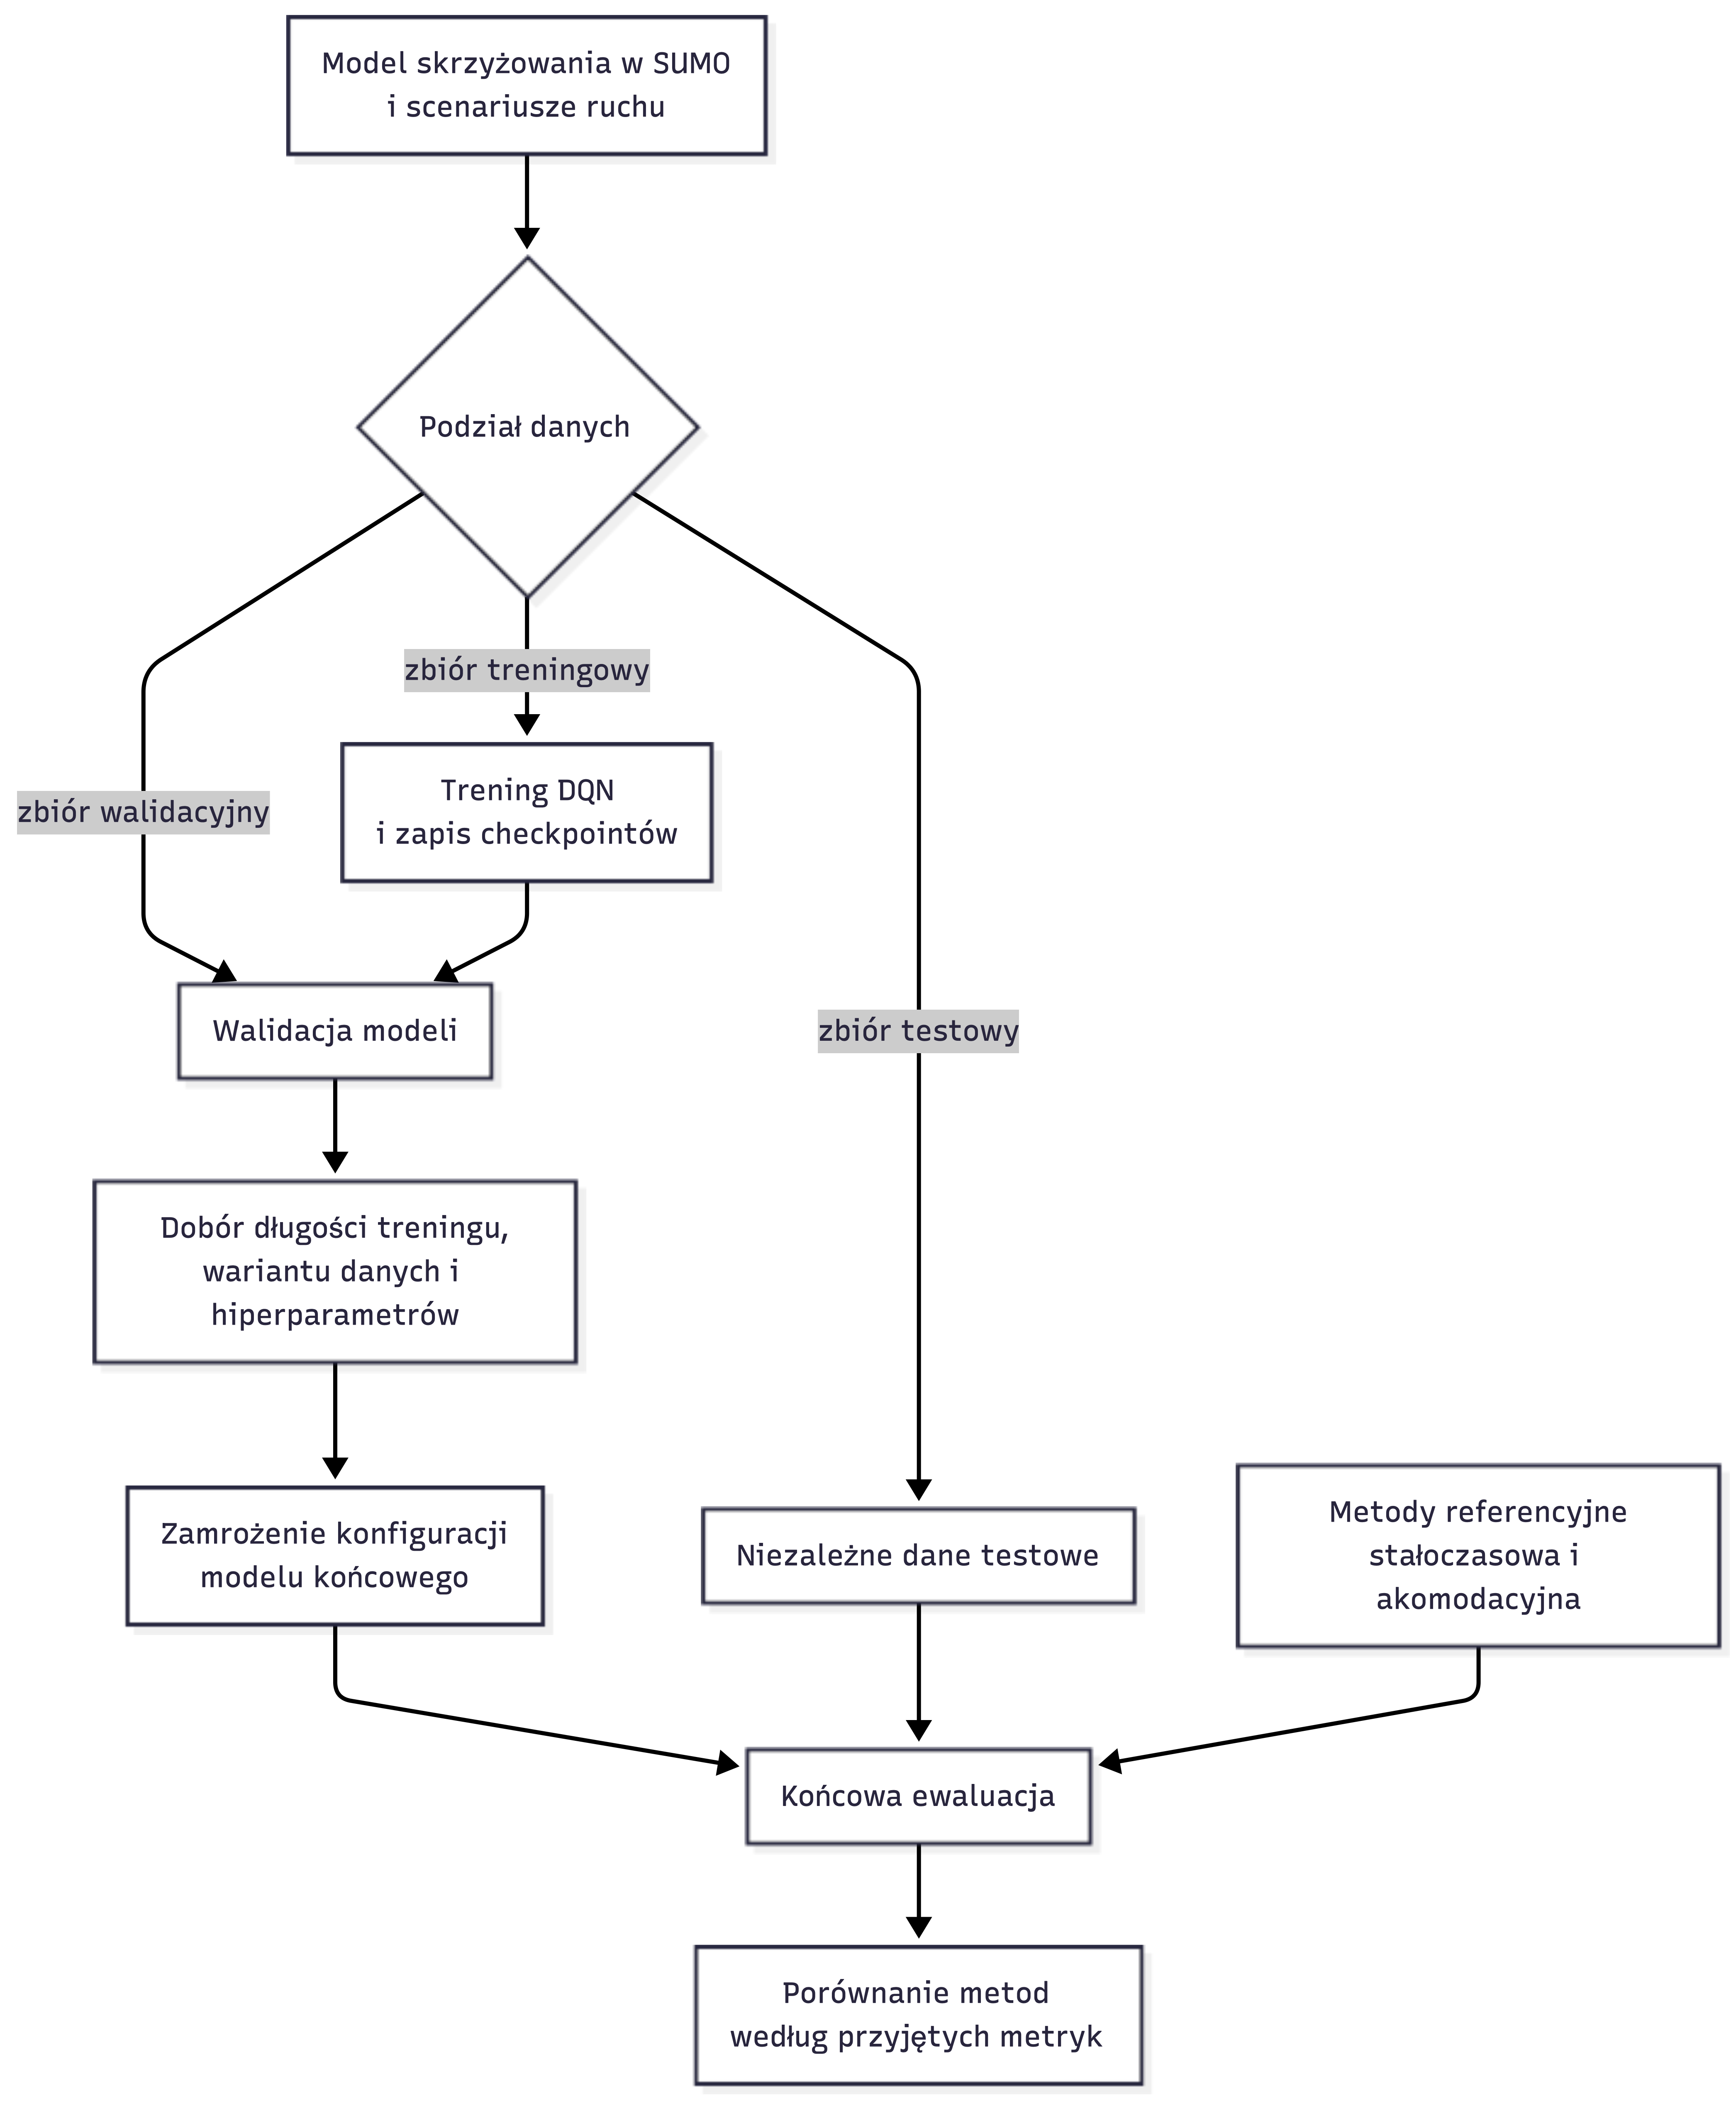
\includegraphics[width=0.65\textwidth]{proces_badawczy.png}
    \caption{Schemat procedury badawczej z rozdzieleniem danych treningowych, walidacyjnych i testowych.}
    \label{fig:proces-badawczy}
\end{figure}

\subsection{Charakterystyka analizowanego skrzyżowania}
\label{subsec:skrzyzowanie}

Do badania wybrano skrzyżowanie ulicy Belgradzkiej z aleją Komisji Edukacji Narodowej, położone w dzielnicy Ursynów w Warszawie. Skrzyżowanie wybrano jako stosunkowo prosty pod względem geometrii, lecz istotnie obciążony układ drogowy, w którym aleja Komisji Edukacji Narodowej stanowi kierunek główny. Położenie skrzyżowania w skali dzielnicy przedstawiono na rysunku~\ref{fig:mapa-ursynow}, a jego bezpośrednie otoczenie na rysunkach~\ref{fig:mapa-osm} oraz~\ref{fig:satelita}.

\begin{figure}[!htbp] \centering
    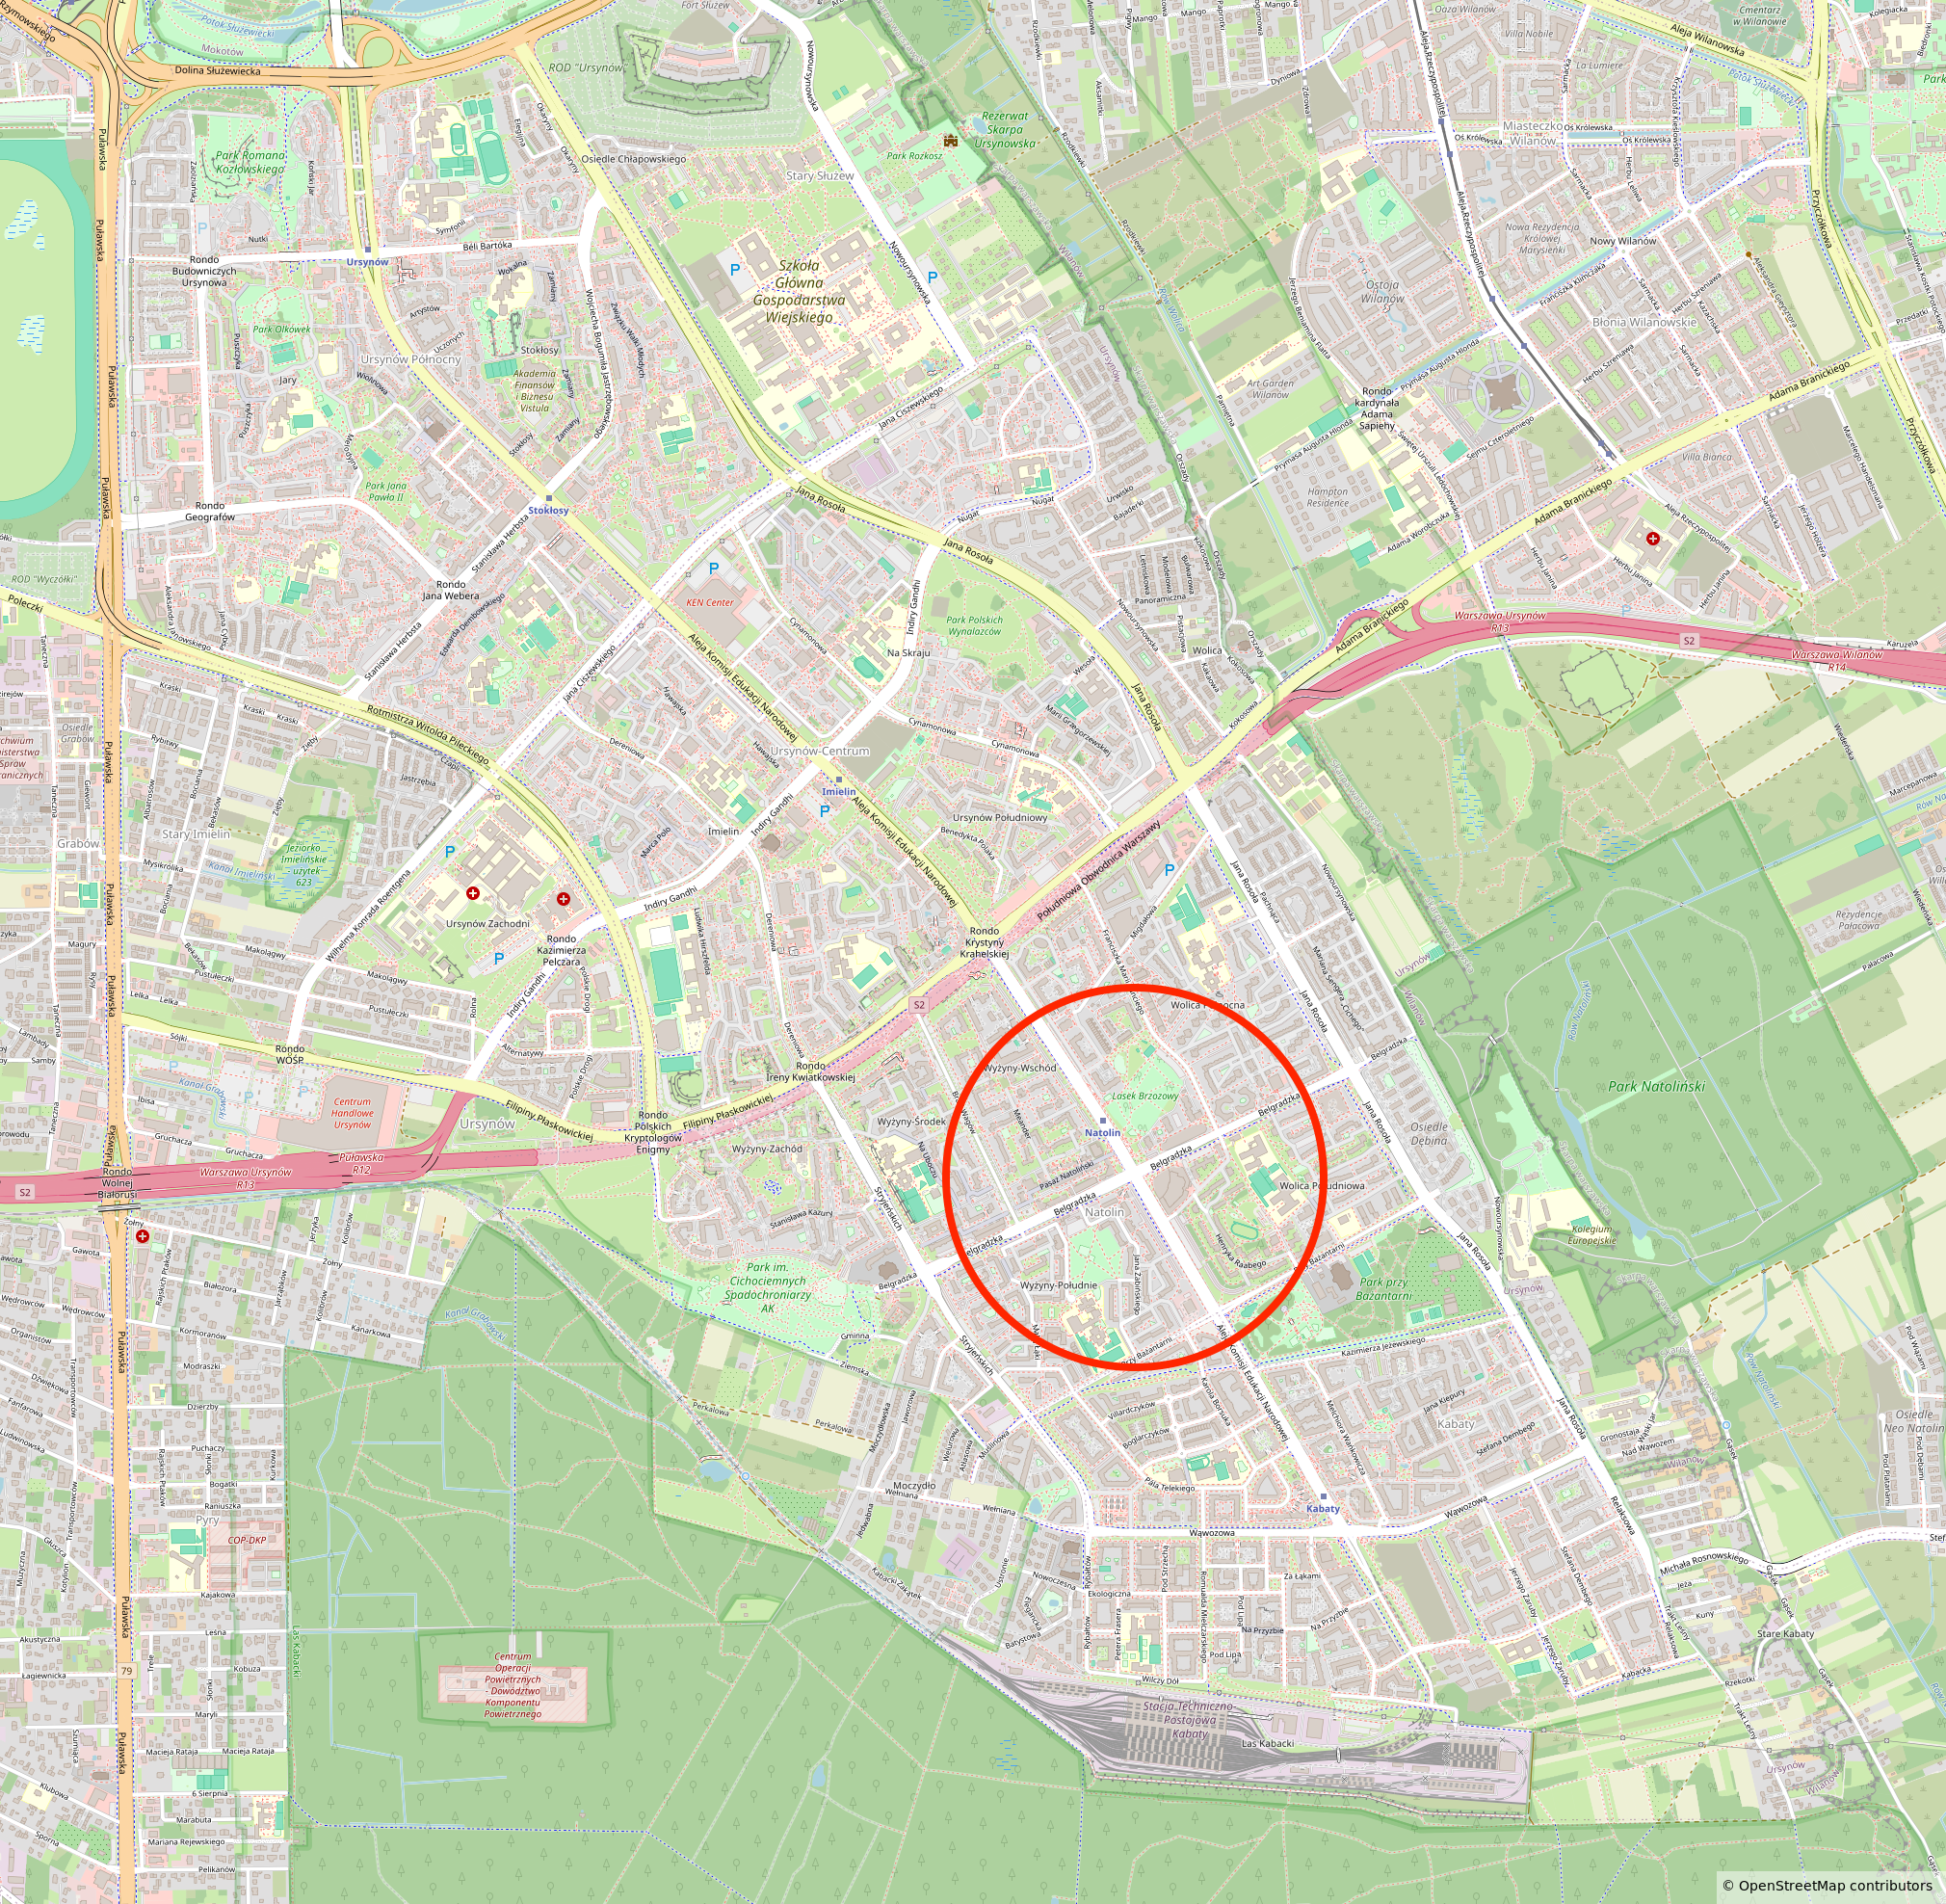
\includegraphics[width=0.75\linewidth]{map-2.png}
    \caption{Położenie analizowanego skrzyżowania na tle warszawskiego Ursynowa. Skrzyżowanie zaznaczono czerwonym okręgiem. Źródło: OpenStreetMap.}
    \label{fig:mapa-ursynow}
\end{figure}

\begin{figure}[!htbp] \centering
    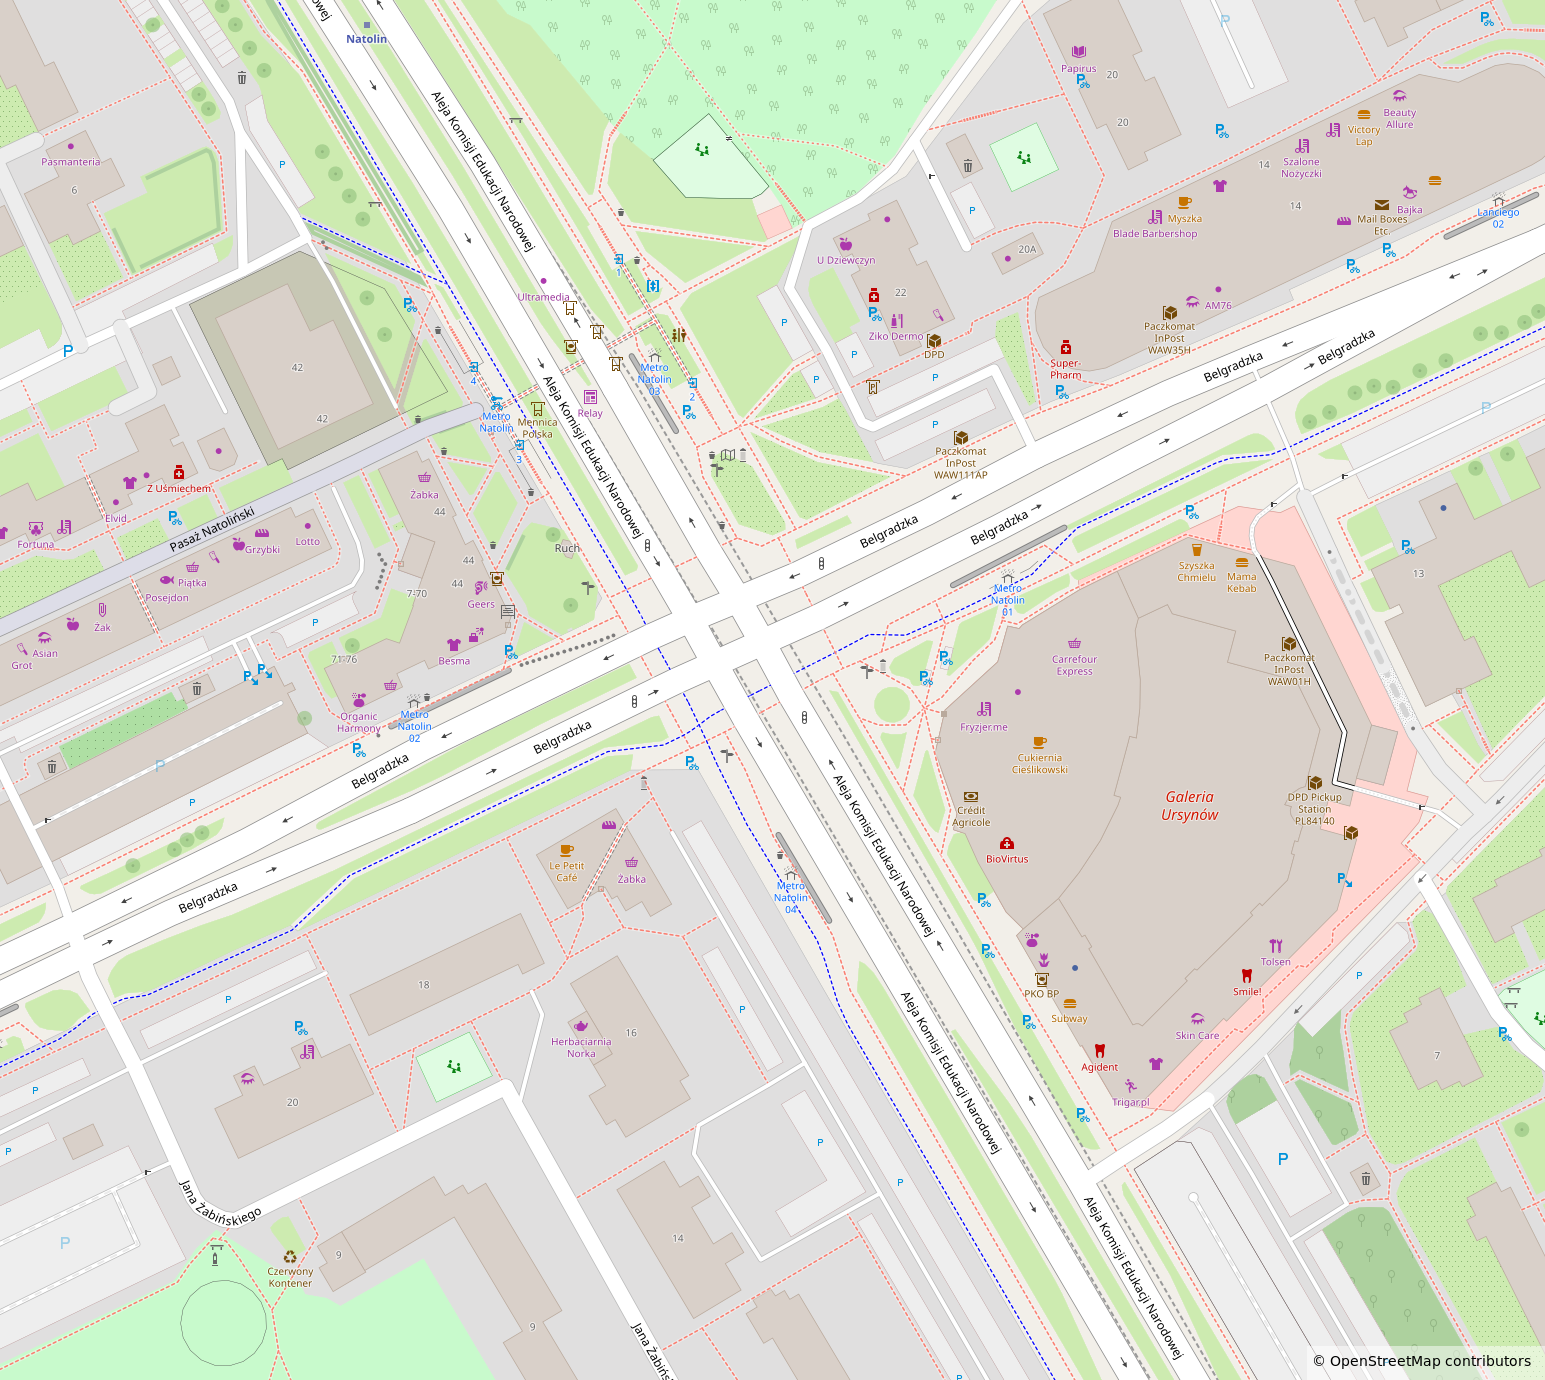
\includegraphics[width=0.75\linewidth]{map.png}
    \caption{Analizowane skrzyżowanie na mapie OpenStreetMap.}
    \label{fig:mapa-osm}
\end{figure}

\begin{figure}[!htbp] \centering
    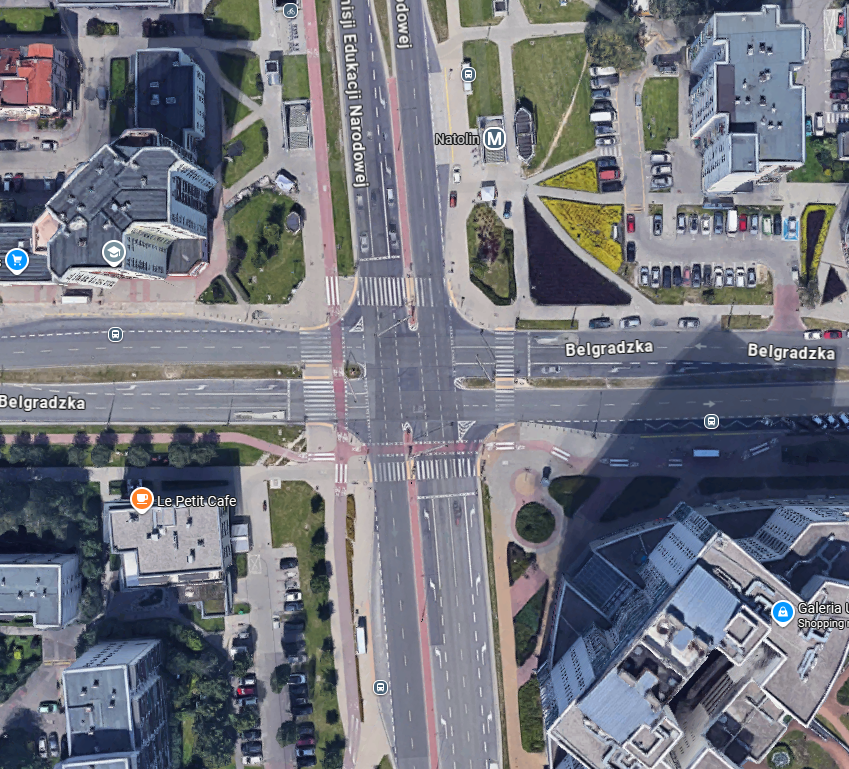
\includegraphics[width=0.75\linewidth]{satelita.png}
    \caption{Widok satelitarny analizowanego skrzyżowania. Źródło: Google Maps.}
    \label{fig:satelita}
\end{figure}

Skrzyżowanie ma cztery wloty, oznaczane w dalszej części pracy jako północny, południowy, wschodni oraz zachodni. Nazwy te odnoszą się do położenia wlotu względem środka skrzyżowania, a nie do kierunku jazdy. Model dopuszcza ruch z każdego wlotu we wszystkich dostępnych kierunkach, z wyłączeniem zawracania. Liczba pasów na poszczególnych wlotach jest zróżnicowana: wlot południowy, z którego pojazdy poruszają się w kierunku północnym, obejmuje cztery pasy, natomiast pozostałe trzy wloty po trzy pasy, co daje łącznie trzynaście pasów wlotowych objętych sterowaniem.

Program sygnalizacji obejmuje trzy fazy z sygnałem zielonym, rozdzielone fazami żółtymi. Pierwsza faza obsługuje jazdę na wprost oraz skręt w prawo na alei Komisji Edukacji Narodowej, jednocześnie z obu kierunków tej osi. Druga faza realizuje skręt w lewo z alei Komisji Edukacji Narodowej, chroniony osobnym sygnałem i rozdzielony w czasie od kolizyjnego strumienia jadącego na wprost z kierunku przeciwnego. Trzecia faza obsługuje ulicę Belgradzką, obejmując jazdę na wprost, skręt w prawo oraz skręt w lewo realizowany warunkowo, to jest przy ustąpieniu pierwszeństwa pojazdom nadjeżdżającym z przeciwka. Różnica w sposobie obsługi lewoskrętów wpływa na przepustowość tych relacji i dlatego jest istotna dla interpretacji wyników.

W modelu odwzorowano geometrię skrzyżowania, liczbę i przeznaczenie pasów ruchu, relacje kolizyjne oraz program sygnalizacji świetlnej. Model zbudowano na podstawie danych OpenStreetMap, a następnie skorygowano na potrzeby eksperymentu. Odwzorowane skrzyżowanie w środowisku SUMO przedstawiono na rysunku~\ref{fig:symulacja}.

\begin{figure}[!htbp] \centering
    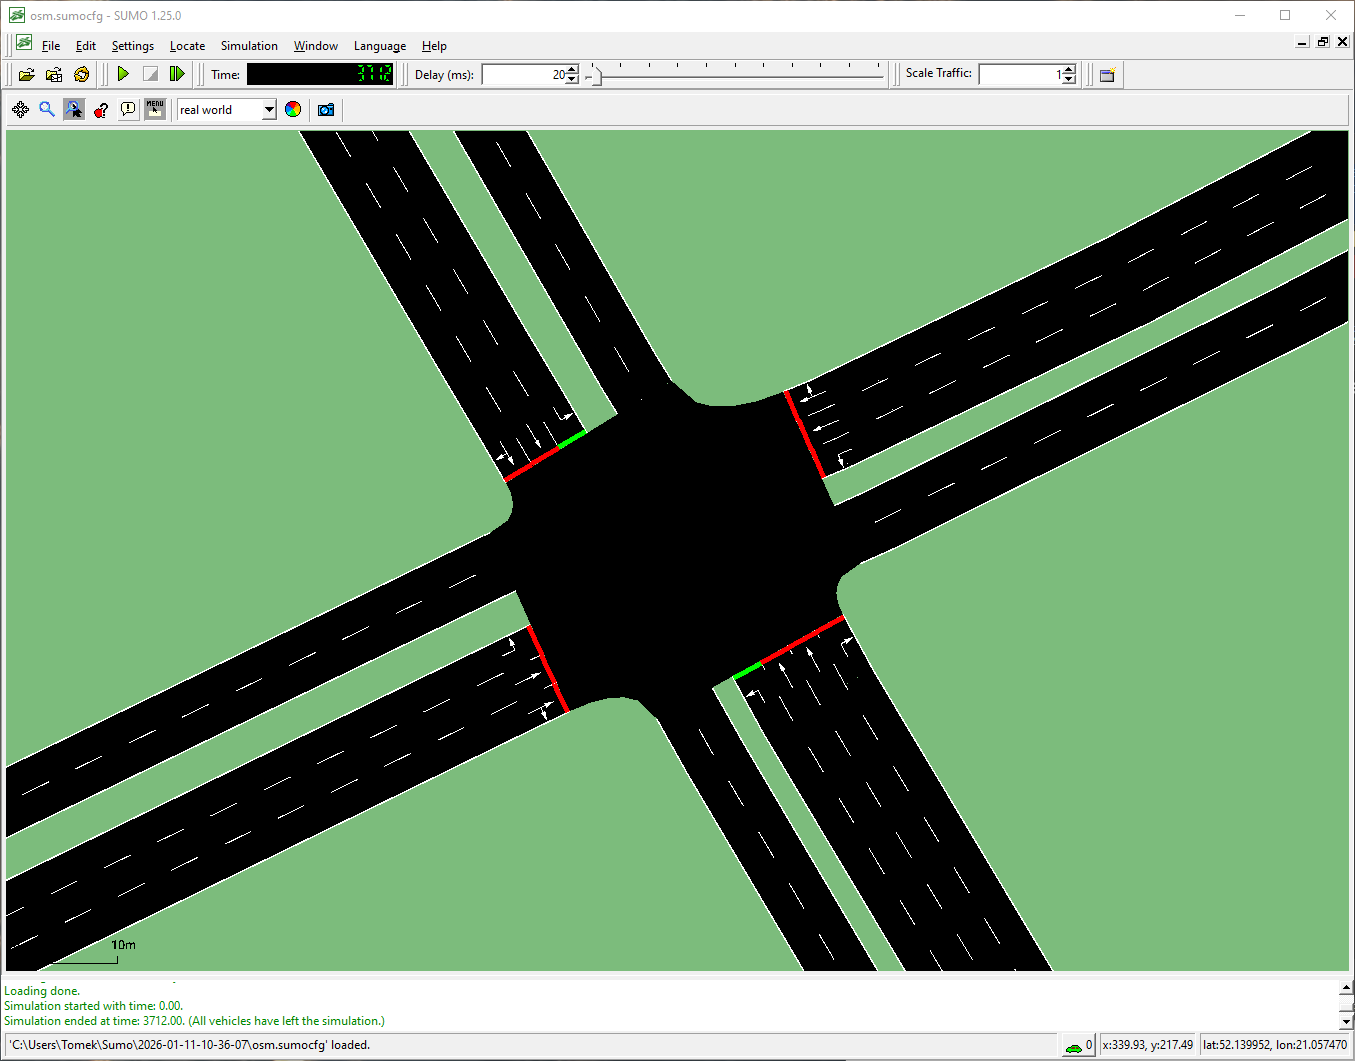
\includegraphics[width=0.8\linewidth]{symulacja.png}
    \caption{Model analizowanego skrzyżowania w środowisku symulacyjnym SUMO.}
    \label{fig:symulacja}
\end{figure}

Zgodnie z ograniczeniami zakresu przedstawionymi w podrozdziale~\ref{subsec:zalozenia-ograniczenia}, model nie obejmuje faz ani ograniczeń czasowych związanych z obsługą przejść dla pieszych.

\subsection{Sformułowanie problemu jako zadania uczenia ze wzmocnieniem}
\label{subsec:sformulowanie-rl}

\subsubsection{Agent i środowisko}
\label{subsubsec:agent-srodowisko}

Problem sterowania sygnalizacją sformułowano jako zadanie uczenia ze wzmocnieniem. Agent odpowiada za wybór fazy sygnalizacji świetlnej, natomiast środowisko stanowi symulacja ruchu drogowego realizowana w SUMO. Komunikację między agentem a symulatorem zapewnia interfejs TraCI, który umożliwia wykonywanie kolejnych kroków symulacji, odczyt stanu ruchu oraz zmianę sygnalizacji.

Warstwę pośredniczącą między symulatorem a algorytmem uczenia stanowi biblioteka \texttt{sumo-rl}, udostępniająca symulację jako środowisko zgodne z interfejsem Gymnasium \cite{alegre2019sumorl}. Na jej podstawie przygotowano własną warstwę integracyjną. Jej architekturę i implementację opisano w rozdziałach~\ref{sec:architektura} oraz~\ref{sec:implementacja}.

\subsubsection{Przestrzeń obserwacji}
\label{subsubsec:obserwacja}

Przestrzeń obserwacji jest ciągła i ma postać \texttt{Box(0.0, 1.0, (30,), float32)}, czyli wektora trzydziestu wartości rzeczywistych z przedziału od 0 do 1. Wykorzystano domyślną reprezentację stanu udostępnianą przez bibliotekę \texttt{sumo-rl} \cite{alegre2019sumorl}, na którą składają się cztery grupy cech:
\begin{itemize}
    \item \emph{kodowanie aktywnej fazy} (3 wartości): wektor zero-jedynkowy typu one-hot wskazujący, która z trzech faz zielonych jest aktualnie realizowana;
    \item \emph{znacznik minimalnego czasu zielonego} (1 wartość): zmienna binarna przyjmująca wartość 1, jeżeli od ostatniej zmiany fazy upłynął już minimalny czas zielony powiększony o czas trwania fazy żółtej, a w przeciwnym razie wartość 0;
    \item \emph{gęstość pasów} (13 wartości): dla każdego z trzynastu pasów wlotowych liczba pojazdów znajdujących się na pasie podzielona przez maksymalną liczbę pojazdów, które mogłyby się na nim zmieścić;
    \item \emph{zapełnienie kolejki} (13 wartości): dla każdego pasa wlotowego liczba pojazdów zatrzymanych, czyli poruszających się z prędkością poniżej 0,1~m/s, podzielona przez tę samą pojemność pasa.
\end{itemize}

Pojemność pasa wyznaczana jest jako jego długość podzielona przez sumę minimalnego odstępu między pojazdami oraz średniej długości pojazdu na tym pasie. Obie ostatnie grupy cech są ograniczone od góry wartością 1, co zapewnia normalizację całego wektora obserwacji do wspólnego zakresu i ułatwia uczenie sieci neuronowej.

Przyjęta reprezentacja opisuje zatem jednocześnie stan sygnalizacji, dopuszczalność zmiany fazy oraz rozkład obciążenia ruchem na poszczególnych pasach wlotowych. Rozdzielenie gęstości i zapełnienia kolejki pozwala odróżnić sytuację, w której pojazdy znajdują się na pasie i płynnie przejeżdżają, od sytuacji, w której pojazdy stoją w kolejce.

\subsubsection{Przestrzeń akcji}
\label{subsubsec:akcje}

Przestrzeń akcji jest dyskretna i ma postać \texttt{Discrete(3)}. Każda akcja odpowiada wskazaniu fazy zielonej, która ma obowiązywać w kolejnym oknie decyzyjnym \cite{alegre2019sumorl}. Trzy dostępne akcje odpowiadają trzem fazom zielonym zdefiniowanym w programie sygnalizacji, opisanym w podrozdziale~\ref{subsec:skrzyzowanie}.

Agent nie steruje bezpośrednio sygnałami na poszczególnych pasach ani nie ustala długości fazy w sposób dowolny. Wskazuje jedynie fazę docelową, natomiast egzekwowanie ograniczeń bezpieczeństwa pozostaje po stronie środowiska. Obowiązują przy tym następujące reguły:
\begin{itemize}
    \item jeżeli agent wskaże fazę identyczną z aktualnie realizowaną, sygnalizacja kontynuuje bieżącą fazę bez żadnej zmiany;
    \item jeżeli agent wskaże fazę inną niż aktualna, lecz od ostatniej zmiany nie upłynął jeszcze minimalny czas zielony powiększony o czas fazy żółtej, żądanie zmiany jest ignorowane i bieżąca faza jest kontynuowana;
    \item jeżeli agent wskaże fazę inną niż aktualna, a warunek czasowy jest spełniony, środowisko wprowadza fazę żółtą jako przejście, a dopiero po jej zakończeniu włącza wskazaną fazę zieloną.
\end{itemize}

Faza żółta jest generowana automatycznie na podstawie porównania stanu sygnałów fazy bieżącej i docelowej, co zapewnia wygaszanie tylko tych relacji, które tracą prawo przejazdu. Mechanizm ten sprawia, że agent nie może przełączać sygnałów natychmiastowo ani z pominięciem czasu międzyzielonego. W eksperymencie przyjęto czas trwania fazy żółtej równy 3~s oraz minimalny czas zielony równy 5~s. Te same wartości obowiązywały podczas treningu, walidacji oraz końcowej oceny na zbiorze testowym, dzięki czemu warunki działania agenta były identyczne na wszystkich etapach eksperymentu.

\subsubsection{Funkcja nagrody}
\label{subsubsec:nagroda}

Wykorzystano funkcję nagrody opartą na zmianie skumulowanego czasu oczekiwania pojazdów \cite{alegre2019sumorl}. W konfiguracji nosi ona nazwę \texttt{diff-waiting-time}. W chwili decyzyjnej $t$ wyznaczana jest wielkość
\begin{equation}
    W_t = \frac{1}{100} \sum_{l \in L} w_{l,t},
    \label{eq:waiting-total}
\end{equation}
gdzie $L$ oznacza zbiór pasów wlotowych sterowanych przez sygnalizację, a $w_{l,t}$ część skumulowanego czasu oczekiwania pojazdów znajdujących się na pasie $l$, przypisaną temu pasowi. Skumulowany czas oczekiwania pojedynczego pojazdu raportowany jest przez SUMO i obejmuje czas, w którym pojazd poruszał się z prędkością poniżej progu zatrzymania. Jeżeli pojazd zmienił pas w obrębie sterowanego obszaru, wykorzystana biblioteka rozdziela tę wielkość między kolejno zajmowane pasy, dzięki czemu ten sam czas oczekiwania nie jest uwzględniany wielokrotnie. Czynnik $\frac{1}{100}$ skaluje sumę do mniejszego zakresu liczbowego. Nagroda przekazywana agentowi jest różnicą między wartością z poprzedniej i bieżącej chwili decyzyjnej:
\begin{equation}
    r_t = W_{t-1} - W_t.
    \label{eq:reward}
\end{equation}

Nagroda jest zatem dodatnia, gdy łączny czas oczekiwania na skrzyżowaniu maleje, a ujemna, gdy rośnie. Agent nie jest uczony bezpośrednio minimalizacji wartości bezwzględnej czasu oczekiwania, lecz podejmowania decyzji prowadzących do jego redukcji względem stanu poprzedniego. Taka konstrukcja daje gęsty sygnał uczący, dostępny po każdej decyzji, co jest korzystne w zadaniu o długim horyzoncie czasowym.

Wybór tej funkcji wynikał z jej bezpośredniego powiązania z jedną z podstawowych metryk oceny jakości sterowania oraz z dostępności sprawdzonej implementacji w wykorzystanej bibliotece. Należy jednak podkreślić, że funkcja nagrody reprezentuje tylko jeden z możliwych sposobów zdefiniowania celu sterowania. Nie uwzględnia ona wprost długości kolejek, przepustowości ani częstotliwości przełączeń sygnalizacji, co należy brać pod uwagę przy interpretacji wyników w pozostałych metrykach.

\subsubsection{Interwał decyzyjny}
\label{subsubsec:interwal}

Agent podejmuje decyzje w stałych odstępach czasu symulacji wynoszących 5~s. Pomiędzy kolejnymi decyzjami symulator wykonuje kroki o długości jednej sekundy, w trakcie których egzekwowane są ograniczenia dotyczące faz oraz rejestrowany jest stan ruchu.

Dobór interwału decyzyjnego stanowi kompromis między częstotliwością reagowania a stabilnością sterowania. Zbyt krótki interwał zwiększa liczbę decyzji przypadających na epizod oraz ryzyko częstych przełączeń sygnalizacji, natomiast zbyt długi ogranicza zdolność agenta do reagowania na zmiany sytuacji ruchowej. Wartość 5~s pozwala agentowi wielokrotnie ocenić sytuację w trakcie trwania jednej fazy, a jednocześnie nie prowadzi do przełączania sygnalizacji częściej, niż dopuszczają to ograniczenia minimalnego czasu zielonego oraz fazy żółtej.

\subsection{Wybór algorytmu}
\label{subsec:wybor-algorytmu}

Punktem wyjścia był klasyczny, tablicowy Q-Learning, opisany w podrozdziale~\ref{subsec:qlearning}. Podejście to odrzucono, ponieważ zastosowanie go do ciągłej, 30-wymiarowej obserwacji wymagałoby dyskretyzacji prowadzącej do niepraktycznie dużej liczby potencjalnych stanów.

Wybrano algorytm Deep Q-Network, który aproksymuje funkcję wartości akcji za pomocą sieci neuronowej \cite{mnih2013playing}. Odpowiada on przyjętemu sformułowaniu zadania, obejmującemu ciągłą obserwację i trzy dyskretne akcje. Wykorzystano implementację ze Stable-Baselines3 oraz politykę \texttt{MlpPolicy}, odpowiednią dla wektorowej reprezentacji obserwacji.

Należy zaznaczyć, że wybór algorytmu DQN nie oznacza, iż jest on rozwiązaniem obiektywnie najlepszym dla rozpatrywanego problemu. Stanowi on natomiast naturalny i uzasadniony wybór przy przyjętym sformułowaniu zadania oraz zakresie pracy.

\subsection{Metody referencyjne}
\label{subsec:metody-referencyjne}

Aby ocena agenta DQN była osadzona w realnym punkcie odniesienia, przygotowano dwie klasyczne metody sterowania. Obie realizują ten sam zbiór faz sygnalizacji co agent, dzięki czemu różnice w wynikach wynikają ze sposobu podejmowania decyzji, a nie z odmiennej organizacji ruchu na skrzyżowaniu.

\subsubsection{Sterowanie stałoczasowe}
\label{subsubsec:ref-staloczasowe}

Sterowanie stałoczasowe stanowi podstawowy punkt odniesienia i w SUMO jest realizowane jako statyczna logika sygnalizacji \cite{sumoTrafficLights}. Czasy faz zielonych wyznaczono proporcjonalnie do natężenia na pasie krytycznym każdej fazy, oszacowanego na podstawie zbioru treningowego. Wynoszą one 14~s, 29~s oraz 29~s, a rozdzielające je fazy żółte trwają po 3~s, co daje cykl o długości 81~s.

\subsubsection{Sterowanie akomodacyjne}
\label{subsubsec:ref-akomodacyjne}

Sterowanie akomodacyjne typu gap-based stanowi bardziej wymagający punkt odniesienia. Może wydłużać aktywną fazę, dopóki detektory rejestrują napływ pojazdów, w granicach minimalnego i maksymalnego czasu zielonego \cite{sumoTrafficLights, NAP22097}. Przyjęto minimum równe 5~s, takie samo jak dla agenta, oraz maksima odpowiadające około półtorakrotności czasów zielonych programu stałoczasowego. Metoda reaguje na ruch według ustalonych reguł, lecz nie uczy się polityki na podstawie doświadczenia.

\subsection{Metryki oceny}
\label{subsec:metryki}

Metody porównywane są według kilku metryk, ponieważ pojedyncza wielkość nie opisuje wszystkich aspektów jakości sterowania. Dane pochodzą z dwóch źródeł: z pliku \texttt{tripinfo.xml} generowanego przez SUMO po zakończeniu symulacji, zawierającego podsumowanie każdej zrealizowanej podróży, oraz z danych rejestrowanych przez interfejs TraCI w każdej sekundzie symulacji. Dla wszystkich metod zastosowano ten sam sposób zbierania i agregacji danych.

\subsubsection{Średnie opóźnienie}
\label{subsubsec:metryka-opoznienie}

Średnie opóźnienie wyznaczane jest jako średnia arytmetyczna wartości \texttt{timeLoss} ze wszystkich zakończonych podróży \cite{sumo_tripinfo_docs}. Wielkość ta określa czas utracony przez pojazd wskutek poruszania się z prędkością niższą od prędkości, z jaką mógłby jechać w warunkach swobodnych. Obejmuje zatem zarówno pełne zatrzymania, jak i zwolnienia wynikające z hamowania oraz przyspieszania.

Metryka wyrażana jest w sekundach na pojazd, a wartości niższe są korzystniejsze. Ze względu na szerokie ujęcie strat czasu metryka ta pełniła wiodącą rolę przy porównywaniu modeli na etapie walidacji.

\subsubsection{Średni czas oczekiwania}
\label{subsubsec:metryka-oczekiwanie}

Wartość \texttt{waitingTime} oznacza czas, w którym pojazd poruszał się poniżej progu uznawanego przez SUMO za zatrzymanie \cite{sumo_tripinfo_docs}. Średni czas oczekiwania jest średnią arytmetyczną tej wartości ze wszystkich zakończonych podróży.

Metryki tej nie należy utożsamiać z opóźnieniem. Opóźnienie obejmuje wszystkie straty czasu, w tym te wynikające ze zwolnienia bez zatrzymania, natomiast czas oczekiwania dotyczy jedynie postoju. Pojazd, który wielokrotnie zwalnia, lecz nigdy się nie zatrzymuje, wykazuje niezerowe opóźnienie przy zerowym czasie oczekiwania. Metryka wyrażana jest w sekundach na pojazd, a wartości niższe są korzystniejsze. Dodatkowo rejestrowano wartość maksymalną oraz kwantyl rzędu 0,95 czasu oczekiwania, opisujące sytuację pojazdów obsłużonych najgorzej.

\subsubsection{Średnia długość kolejki}
\label{subsubsec:metryka-kolejka}

Długość kolejki wyznaczana jest na podstawie danych rejestrowanych w każdej sekundzie symulacji. W każdym kroku zliczana jest liczba pojazdów zatrzymanych na trzynastu pasach wlotowych, przy czym za pojazd należący do kolejki uznawany jest pojazd poruszający się z prędkością poniżej progu zatrzymania stosowanego przez SUMO \cite{sumo_lane_docs}. Wartości sumowane są w obrębie czterech wlotów, a następnie uśredniane po wszystkich krokach symulacji.

Metryka wyrażana jest w pojazdach, a wartości niższe są korzystniejsze. Poza wartością średnią rejestrowano również wartość maksymalną oraz wartości w podziale na poszczególne wloty, co pozwala ocenić, czy sterowanie nie poprawia sytuacji na jednym wlocie kosztem pozostałych.

\subsubsection{Przepustowość}
\label{subsubsec:metryka-przepustowosc}

Przepustowość wyznaczana jest na podstawie liczby podróży zakończonych w trakcie symulacji, czyli pojazdów, które opuściły sieć drogową. Liczba ta jest dzielona przez czas od najwcześniejszego wyjazdu do najpóźniejszego przyjazdu wśród zakończonych podróży, a następnie przeliczana na godzinę zgodnie z zależnością
\begin{equation}
    Q = \frac{N}{t_{\max} - t_{\min}} \cdot 3600,
    \label{eq:throughput}
\end{equation}
gdzie $N$ oznacza liczbę zakończonych podróży, $t_{\min}$ najwcześniejszy czas wyjazdu w tym zbiorze, a $t_{\max}$ najpóźniejszy czas przyjazdu.

Metryka wyrażana jest w pojazdach na godzinę i jest jedyną z rozpatrywanych, dla której wartości wyższe są korzystniejsze. Należy zaznaczyć, że przy zadanym z góry napływie pojazdów metryka ta służy przede wszystkim do wykrycia sytuacji, w której sterowanie nie jest w stanie obsłużyć zgłaszanego popytu.

\subsubsection{Częstotliwość przełączeń}
\label{subsubsec:metryka-przelaczenia}

Częstotliwość przełączeń opisuje, jak często zmienia się układ sygnałów na skrzyżowaniu. Za przełączenie uznawane jest przejście między dwiema różnymi konfiguracjami sygnału zielonego. Fazy żółte, stanowiące jedynie przejście między fazami zielonymi, nie są liczone jako osobne przełączenia, dzięki czemu jedna zmiana fazy nie jest zliczana dwukrotnie. Liczba przełączeń dzielona jest przez czas między pierwszym i ostatnim rekordem szeregu czasowego, a następnie przeliczana na godzinę.

Metryka wyrażana jest w przełączeniach na godzinę. W jej przypadku nie można wskazać jednoznacznie pożądanego kierunku zmian. Zbyt rzadkie przełączanie oznacza wydłużone oczekiwanie na wlotach nieobsługiwanych, natomiast zbyt częste prowadzi do narastania czasów międzyzielonych, w których żaden strumień nie korzysta ze skrzyżowania, a także obniża komfort i przewidywalność jazdy. Metryka ta pełni zatem rolę kontrolną i pozwala ocenić, czy poprawa pozostałych wskaźników nie została osiągnięta kosztem niestabilnego sterowania.

\subsection{Podział danych eksperymentalnych}
\label{subsec:podzial-danych}

Scenariusze ruchu wygenerowano przy użyciu skryptu \texttt{randomTrips.py}, dostarczanego wraz z SUMO \cite{sumo_randomtrips_docs}. Natężenie ruchu regulowano parametrem określającym średni odstęp między kolejnymi wyjazdami pojazdów, a zróżnicowanie układu tras zapewniono przez zmianę ziarna generatora liczb losowych. Wygenerowane podróże przekształcano następnie na poprawne trasy w analizowanej sieci.

Dane podzielono na trzy rozłączne zbiory: treningowy, walidacyjny i testowy. Podział ten przedstawiono na rysunku~\ref{fig:podzial-danych}.

\begin{figure}[!htbp] \centering
    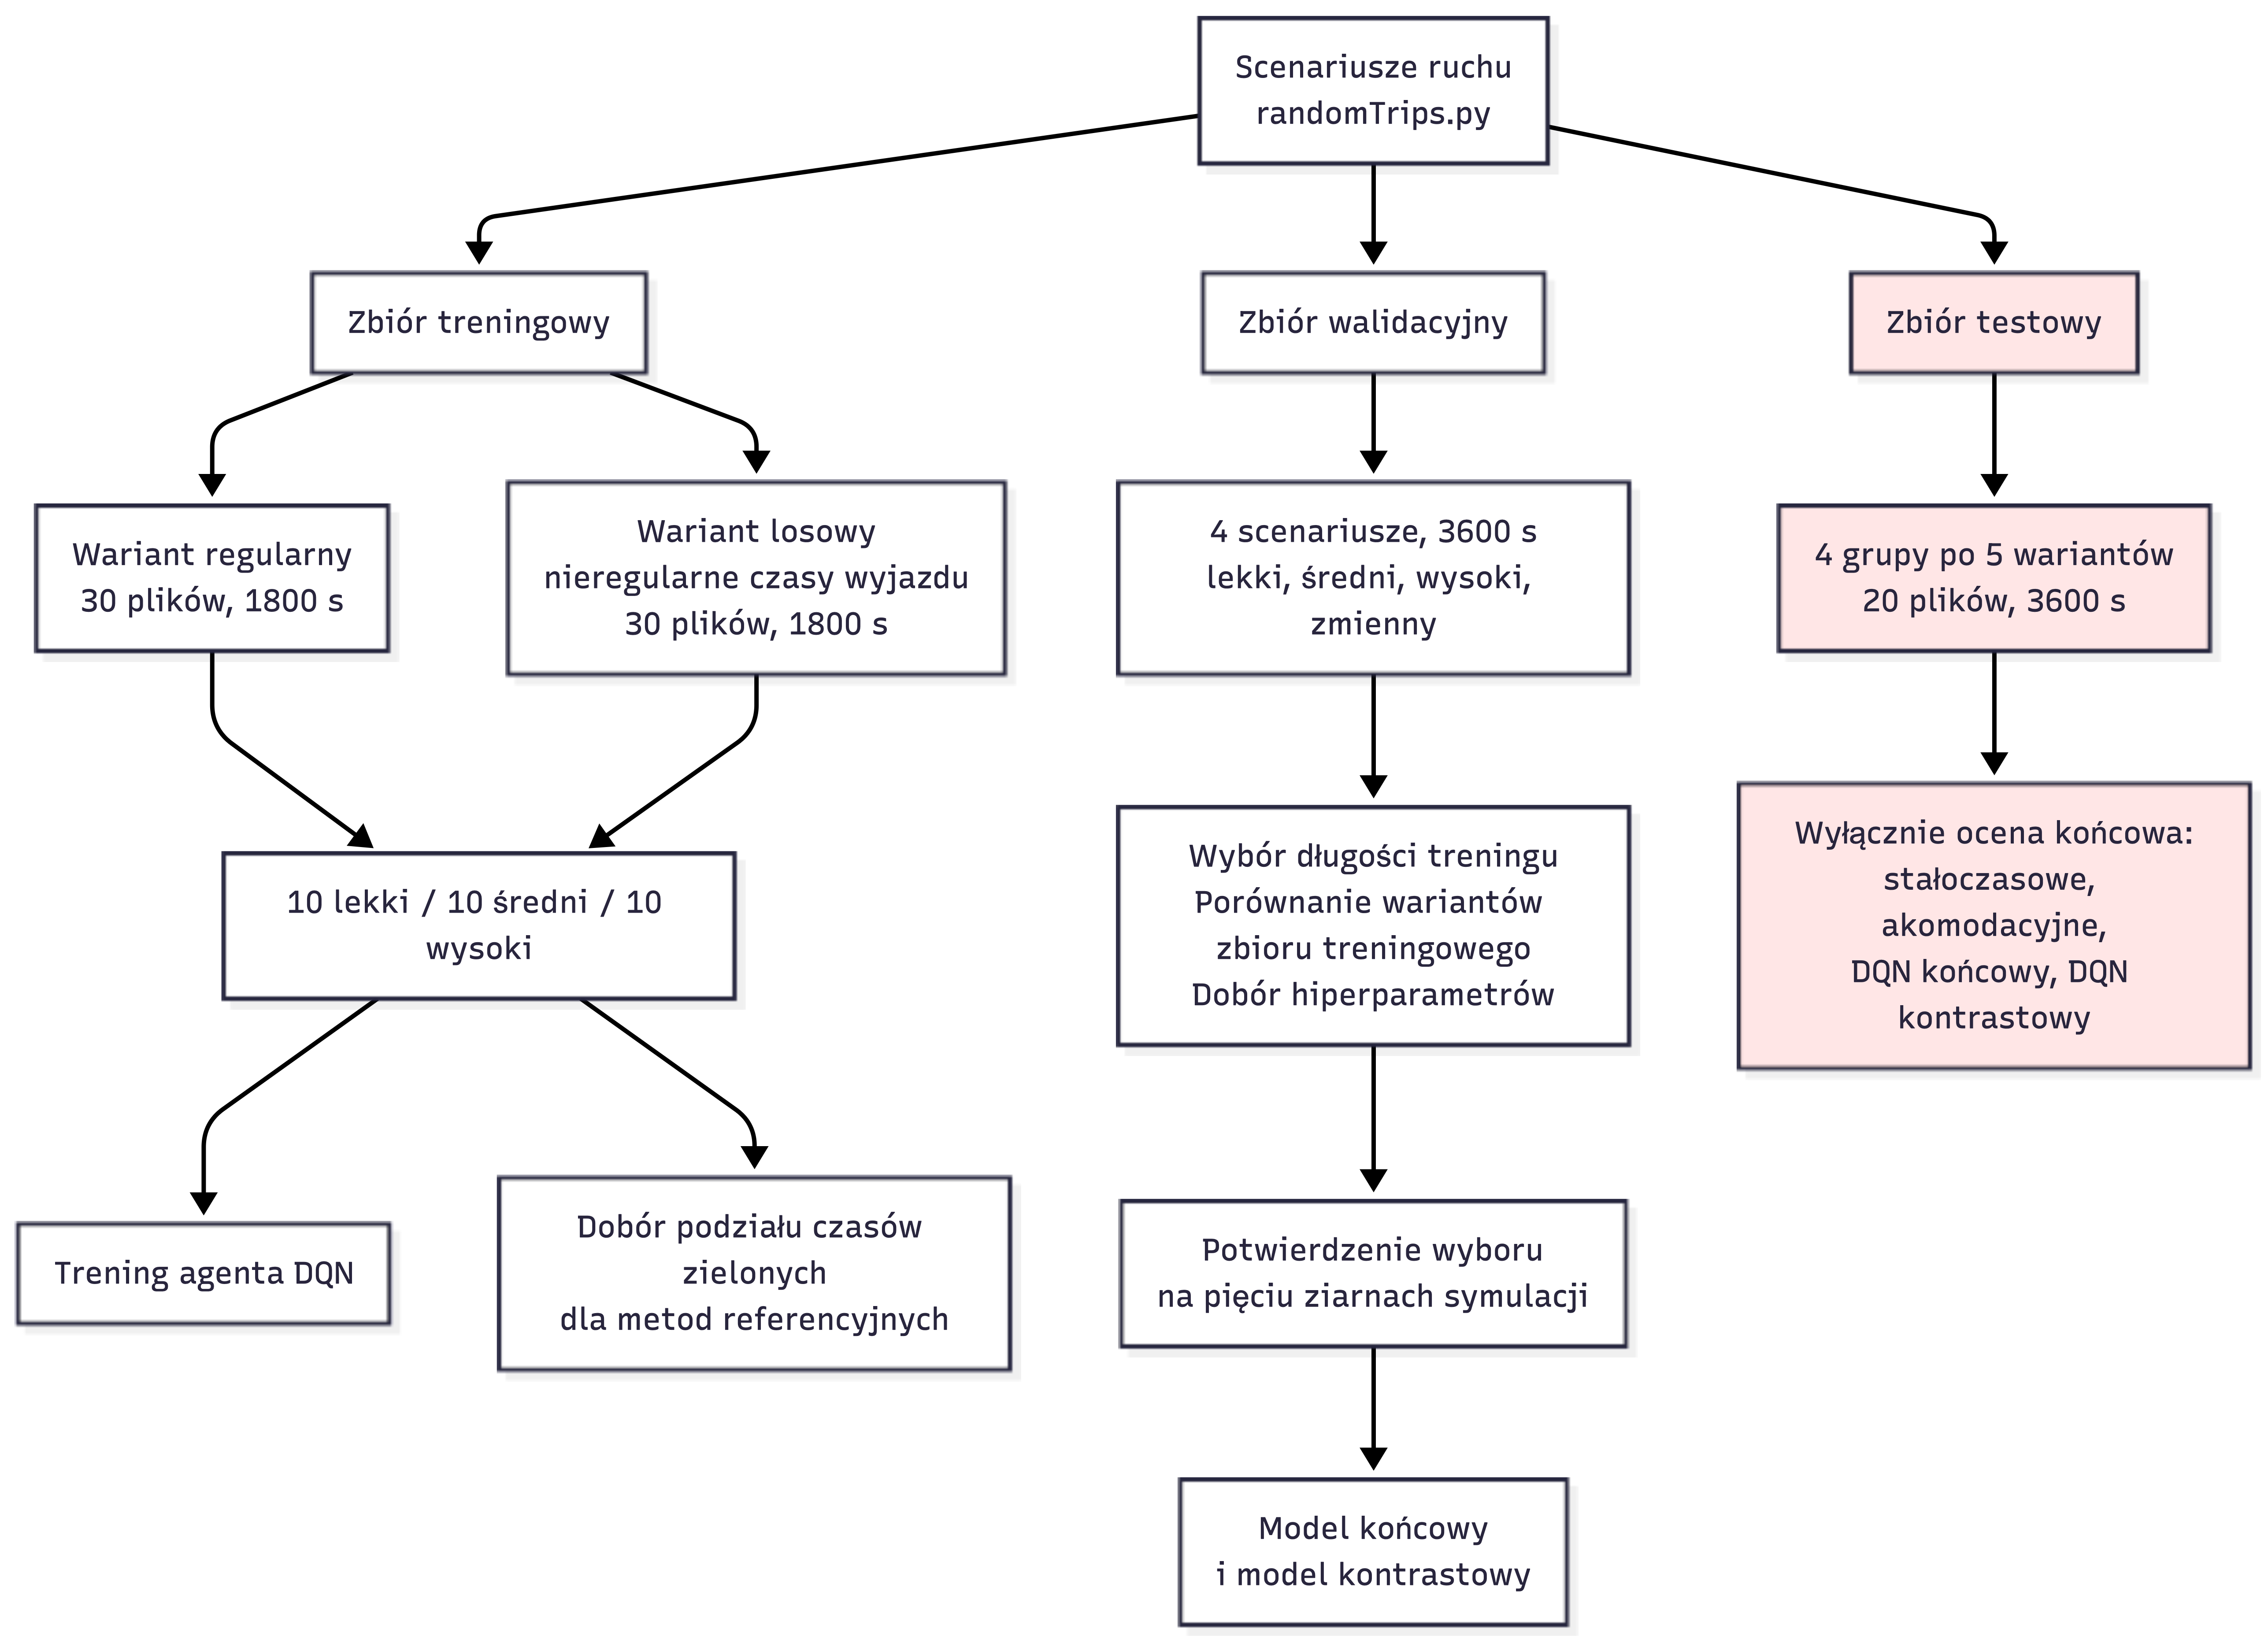
\includegraphics[width=\linewidth]{podzial_danych.png}
    \caption{Podział danych eksperymentalnych oraz przeznaczenie poszczególnych zbiorów.}
    \label{fig:podzial-danych}
\end{figure}

\subsubsection{Zbiór treningowy}
\label{subsubsec:zbior-treningowy}

Przygotowano dwa warianty zbioru treningowego, różniące się sposobem rozmieszczenia czasów wyjazdu pojazdów. Celem było sprawdzenie, czy większa nieregularność napływu pojazdów w danych treningowych poprawia zdolność modelu do generalizacji.

Pierwszy wariant obejmuje scenariusze o regularnych odstępach między wyjazdami, generowane dla zadanego okresu napływu. Drugi wariant obejmuje scenariusze o zbliżonych poziomach natężenia, lecz z nieregularnymi czasami wyjazdu, uzyskanymi przez zastosowanie opcji \texttt{--random-depart} oraz dodatkowego różnicowania napływu pojazdów.

Każdy z wariantów zawiera 30 plików tras, po 10 plików dla każdego z trzech poziomów natężenia ruchu: lekkiego, średniego oraz wysokiego. Każdy scenariusz treningowy obejmuje 1800~s napływu pojazdów, natomiast epizod trwa 2100~s, aby umożliwić opróżnienie sieci. Poszczególne pliki różnią się ziarnem generatora liczb losowych. Podczas treningu kolejne epizody wykorzystują kolejne pliki tras, dzięki czemu agent styka się z różnymi układami tras oraz różnymi poziomami obciążenia.

\subsubsection{Zbiór walidacyjny}
\label{subsubsec:zbior-walidacyjny}

Zbiór walidacyjny obejmuje cztery scenariusze: trzy odpowiadające stałym poziomom natężenia ruchu, to jest lekkiemu, średniemu i wysokiemu, oraz jeden scenariusz dynamiczny, w którym poziom obciążenia zmienia się w trakcie symulacji. Każdy scenariusz walidacyjny obejmuje 3600~s napływu pojazdów.

Zbiór ten wykorzystano do podejmowania wszystkich decyzji dotyczących konfiguracji modelu, a w szczególności do:
\begin{itemize}
    \item wyboru odpowiedniej liczby kroków treningowych na podstawie oceny kolejnych checkpointów;
    \item porównania obu wariantów zbioru treningowego;
    \item doboru hiperparametrów algorytmu;
    \item oceny stabilności procesu uczenia;
    \item wyboru modelu końcowego.
\end{itemize}

\subsubsection{Zbiór testowy}
\label{subsubsec:zbior-testowy}

Zbiór testowy obejmuje cztery grupy scenariuszy, odpowiadające trzem stałym poziomom natężenia ruchu oraz scenariuszowi o zmiennym natężeniu. W każdej grupie przygotowano pięć wariantów różniących się ziarnem generatora liczb losowych, co daje łącznie 20 plików tras. Każdy scenariusz testowy obejmuje 3600~s napływu pojazdów.

Zastosowanie pięciu wariantów w obrębie każdej grupy pozwala ograniczyć wpływ pojedynczego, korzystnego lub niekorzystnego układu tras na wnioski. Wyniki przedstawiane są zatem jako wartości uśrednione wraz z miarą rozrzutu, a nie jako pojedyncze przebiegi. Te same pliki tras wykorzystano do oceny wszystkich trzech porównywanych metod sterowania.

\subsubsection{Zapobieganie przenikaniu danych}
\label{subsubsec:przenikanie-danych}

Rozdzielenie zbiorów jest istotnym elementem metodyki, ponieważ wielokrotne korzystanie z tych samych danych na etapie strojenia i oceny prowadziłoby do zawyżenia wyników i utraty wiarygodności wniosków. W eksperymencie przyjęto następujące zasady:
\begin{itemize}
    \item wszystkie decyzje dotyczące liczby kroków treningowych, wyboru zbioru treningowego oraz wartości hiperparametrów podejmowano wyłącznie na podstawie wyników na zbiorze walidacyjnym;
    \item parametry czasowe metod referencyjnych, to jest czasy trwania faz programu stałoczasowego oraz ograniczenia czasowe sterowania akomodacyjnego, wyznaczono wyłącznie na podstawie scenariuszy ze zbioru treningowego;
    \item konfigurację modelu końcowego ustalono i zamrożono przed jego pierwszą ewaluacją na zbiorze testowym;
    \item zbioru testowego nie wykorzystywano podczas treningu ani strojenia, a jego scenariusze zostały wygenerowane z użyciem ziaren niezależnych od pozostałych zbiorów;
    \item po obejrzeniu wyników testowych nie wprowadzano zmian w modelu ani w jego konfiguracji.
\end{itemize}

\clearpage
\section{Architektura systemu}
\label{sec:architektura}

Rozdział przedstawia system od strony komponentów, ich odpowiedzialności oraz zależności między nimi. Szczególną uwagę poświęcono rozmieszczeniu poszczególnych elementów w warstwach systemu oraz przepływowi danych między nimi.

\subsection{Ogólna architektura rozwiązania}
\label{subsec:ogolna-architektura}

System zbudowano warstwowo. Każda warstwa odpowiada za wyraźnie wyodrębniony zakres zadań i komunikuje się wyłącznie z warstwami sąsiednimi. Ogólny układ komponentów oraz przepływ pojedynczej decyzji przedstawiono na rysunku~\ref{fig:architektura}.

Wyróżnić można następujące elementy:
\begin{itemize}
    \item \emph{dane wejściowe}, czyli pliki opisujące sieć drogową, scenariusze ruchu oraz konfigurację symulacji;
    \item \emph{symulator SUMO}, odpowiedzialny za mikroskopowy model ruchu oraz wykonywanie kolejnych kroków symulacji;
    \item \emph{interfejs TraCI}, zapewniający dwukierunkową komunikację między procesem symulacji a kodem w języku Python;
    \item \emph{bibliotekę \texttt{sumo-rl}}, udostępniającą symulację jako środowisko uczenia ze wzmocnieniem oraz realizującą maszynę stanów sygnalizacji;
    \item \emph{własną warstwę integracyjną}, dostosowującą przebieg pojedynczego kroku środowiska oraz sposób zbierania danych;
    \item \emph{algorytm DQN} z biblioteki Stable-Baselines3, realizujący uczenie oraz wybór akcji;
    \item \emph{moduł zbierania metryk}, rejestrujący stan ruchu w każdej sekundzie symulacji i wyznaczający wielkości podsumowujące;
    \item \emph{moduł zapisu modeli i wyników}, obsługujący checkpointy, modele końcowe oraz pliki wynikowe;
    \item \emph{moduł ewaluacyjny}, uruchamiający zapisany model na zadanym scenariuszu i zapisujący wynik w ujednoliconym formacie.
\end{itemize}

\begin{figure}[!htbp]
    \centering
    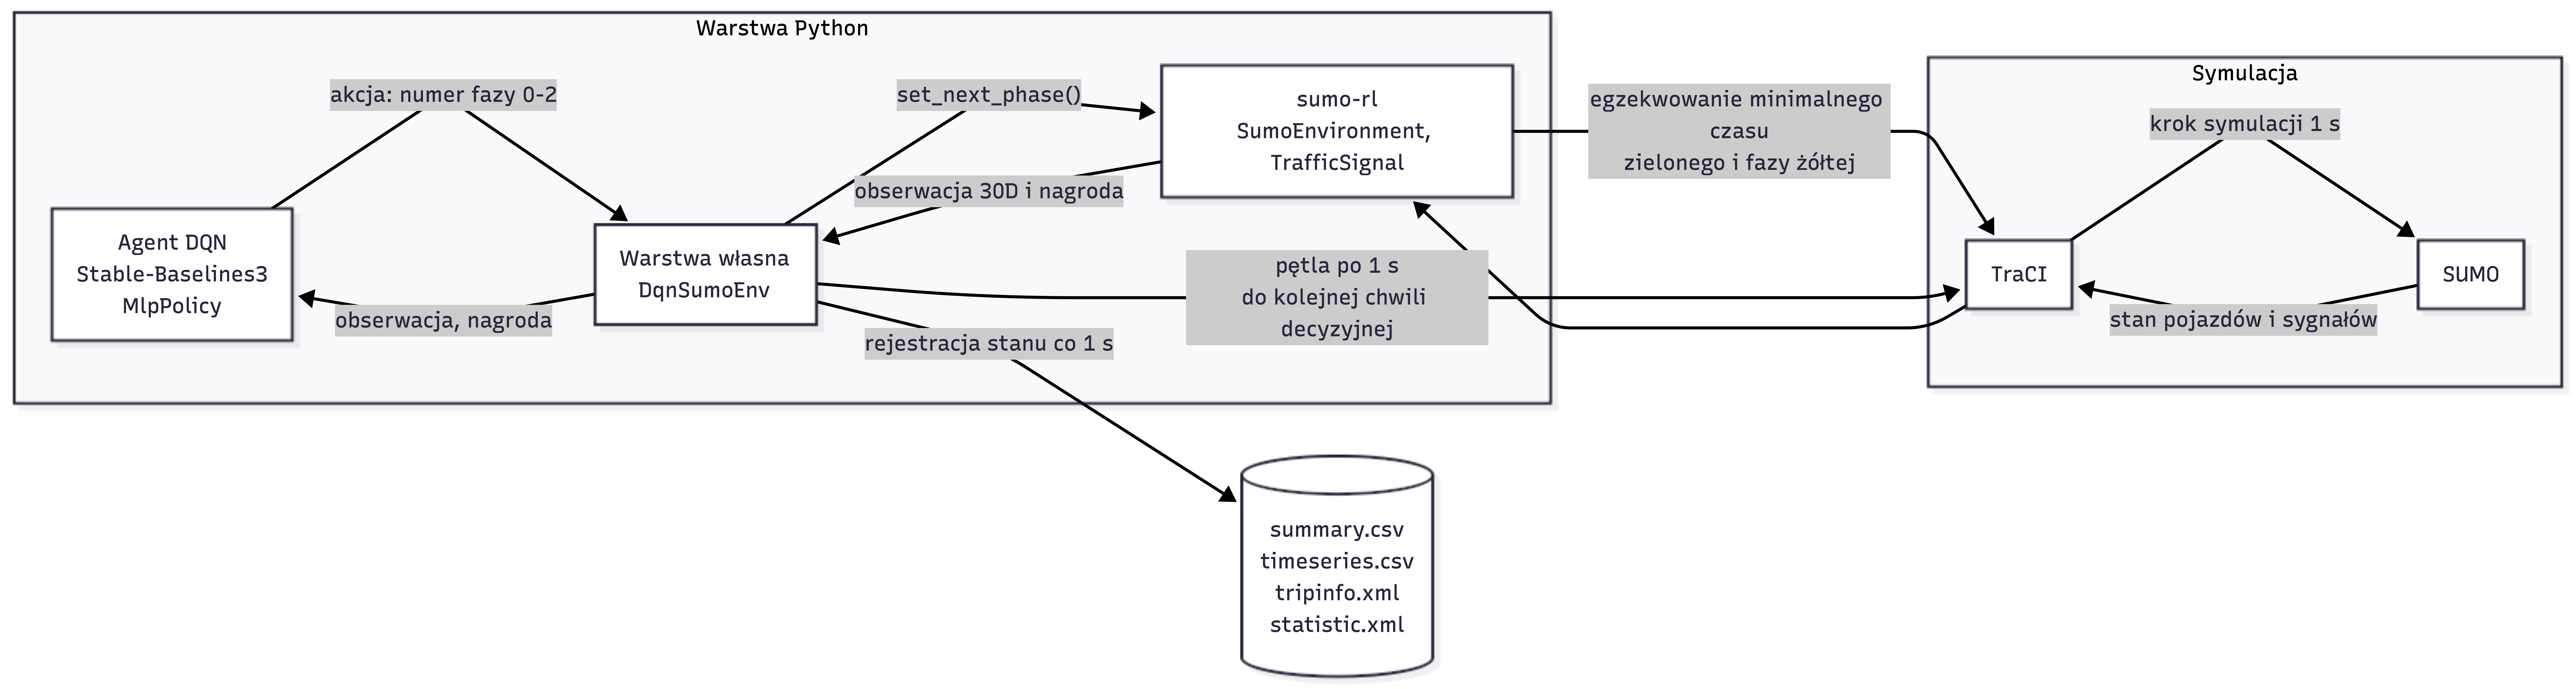
\includegraphics[width=\linewidth]{architektura_systemu.png}
    \caption{Architektura systemu oraz przepływ pojedynczej decyzji agenta.}
    \label{fig:architektura}
\end{figure}

Podział ten oddziela model ruchu od algorytmu uczenia, dzięki czemu zmiana scenariusza lub programu sygnalizacji nie wymaga modyfikacji kodu agenta. Pozwala również stosować spójną procedurę zbierania i agregacji metryk dla wszystkich metod.

Metody referencyjne, przedstawione w podrozdziale~\ref{subsec:metody-referencyjne}, korzystają z tej samej infrastruktury z pominięciem warstw uczenia ze wzmocnieniem. Ich logika działania realizowana jest wewnątrz SUMO, a kod w języku Python pełni jedynie rolę obserwatora, który wykonuje kolejne kroki symulacji przez TraCI i rejestruje te same wielkości co w przypadku agenta.

\subsection{Środowisko symulacyjne SUMO}
\label{subsec:sumo}

SUMO (ang. Simulation of Urban MObility) jest otwartym pakietem do mikroskopowej symulacji ruchu drogowego \cite{lopez2018sumo}. Symulacja mikroskopowa oznacza, że każdy pojazd modelowany jest indywidualnie, wraz z własną trasą, parametrami dynamiki oraz decyzjami dotyczącymi przyspieszania, hamowania i zmiany pasa. W odróżnieniu od modeli makroskopowych, opisujących ruch wielkościami zagregowanymi, takimi jak natężenie czy gęstość potoku, podejście mikroskopowe pozwala wyznaczyć wielkości dotyczące pojedynczych podróży, na przykład czas utracony lub czas postoju konkretnego pojazdu. Jest to warunek konieczny do wyznaczenia metryk przyjętych w pracy.

W systemie SUMO pełni rolę modelu środowiska. Odpowiada za geometrię sieci drogowej, ruch i dynamikę pojazdów, realizację wyznaczonych tras, wykonanie logiki sygnalizacji świetlnej oraz udostępnienie danych potrzebnych do wyznaczenia obserwacji, nagrody i metryk. Sam symulator nie zawiera żadnych elementów uczenia maszynowego, a jego stan zmienia się wyłącznie w wyniku kolejnych kroków symulacji.

Konfigurację eksperymentu opisują pliki w formacie XML:
\begin{itemize}
    \item pliki sieci drogowej z rozszerzeniem \texttt{.net.xml}, zawierające odcinki dróg, pasy ruchu, węzły, relacje kolizyjne oraz definicje programów sygnalizacji;
    \item pliki tras z rozszerzeniem \texttt{.rou.xml}, opisujące pojazdy, ich czasy wyjazdu oraz ciągi odcinków, którymi się poruszają;
    \item pliki konfiguracyjne z rozszerzeniem \texttt{.sumocfg}, wiążące sieć z plikami tras oraz ustawiające opcje przetwarzania i raportowania;
\end{itemize}

W eksperymencie wykorzystano dwa pliki sieci o identycznej geometrii i identycznym układzie faz, różniące się wyłącznie typem logiki sygnalizacji. Plik z logiką statyczną obsługuje sterowanie stałoczasowe, natomiast plik z logiką akomodacyjną obsługuje metodę referencyjną typu gap-based. Każdej z trzech porównywanych metod odpowiada osobny plik konfiguracyjny, dzięki czemu wybór metody sterowania sprowadza się do wskazania innej konfiguracji, bez modyfikowania danych wejściowych. Plik tras podawany jest natomiast z wiersza poleceń, ponieważ ta sama konfiguracja wykorzystywana jest dla wielu scenariuszy różniących się ziarnem generatora.

Po zakończeniu symulacji SUMO zapisuje plik \texttt{tripinfo.xml}, zawierający opis każdej zakończonej podróży \cite{sumo_tripinfo_docs}. Stanowi on jedno z dwóch źródeł metryk opisanych w podrozdziale~\ref{subsec:metryki}; drugim są dane odczytywane podczas symulacji przez TraCI.

\subsection{Interfejs TraCI}
\label{subsec:traci}

TraCI (ang. Traffic Control Interface) jest interfejsem umożliwiającym sterowanie działającą symulacją SUMO z poziomu zewnętrznego programu \cite{sumo_traci_docs}. Symulator działa wówczas jako serwer, a program sterujący jako klient łączący się z nim przez gniazdo sieciowe. Rozwiązanie to pozwala zatrzymać symulację po każdym kroku, odczytać jej stan oraz zmienić parametry przed wykonaniem kroku następnego.

W systemie TraCI stanowi jedyną granicę między symulatorem a kodem w języku Python. Realizowane są przez niego cztery grupy operacji:
\begin{itemize}
    \item \emph{wykonywanie kroków symulacji}: sterowanie postępem czasu symulacji krokami o długości jednej sekundy oraz sprawdzanie, czy w sieci pozostały jeszcze pojazdy oczekujące na obsługę, co pozwala wykryć naturalne zakończenie scenariusza;
    \item \emph{odczyt stanu ruchu}: pobranie dla wskazanych pasów wlotowych liczby pojazdów, liczby pojazdów zatrzymanych oraz skumulowanych czasów oczekiwania, czyli wielkości, na podstawie których wyznaczane są obserwacja, nagroda oraz długość kolejki;
    \item \emph{odczyt stanu sygnalizacji}: pobranie łańcucha znaków opisującego bieżący sygnał dla każdej relacji sterowanej przez sygnalizator, wykorzystywanego przy zliczaniu przełączeń;
    \item \emph{zmiana sygnalizacji}: ustawienie nowego układu sygnałów, dzięki czemu decyzja agenta zostaje wprowadzona do symulacji.
\end{itemize}

W przypadku metod referencyjnych TraCI wykorzystywany jest wyłącznie do odczytu stanu oraz do wykonywania kolejnych kroków symulacji. Logika sterowania pozostaje po stronie SUMO, dzięki czemu metody klasyczne działają dokładnie tak, jak zdefiniowano je w pliku sieci.

\subsection{Biblioteka \texttt{sumo-rl}}
\label{subsec:sumo-rl}

Biblioteka \texttt{sumo-rl} pośredniczy między symulacją SUMO a algorytmem uczenia ze wzmocnieniem \cite{alegre2019sumorl}. Jej podstawowym elementem jest klasa \texttt{SumoEnvironment}. Uruchamia ona symulację, nawiązuje połączenie przez TraCI i udostępnia środowisko zgodne z interfejsem Gymnasium \cite{towers2025gymnasium}. Interfejs ten definiuje rozpoczęcie epizodu i wykonanie kroku w odpowiedzi na akcję, a także deklaracje przestrzeni obserwacji i akcji.

Biblioteka realizuje w systemie następujące zadania:
\begin{itemize}
    \item uruchamianie i zamykanie procesu symulacji wraz z przekazaniem opcji wiersza poleceń, w tym ziarna generatora oraz ścieżek plików wyjściowych;
    \item odczytanie z pliku sieci zbioru faz zielonych sterowanego sygnalizatora i zbudowanie na tej podstawie własnej maszyny stanów, wraz z automatycznym generowaniem faz żółtych;
    \item egzekwowanie ograniczeń czasowych, to jest minimalnego czasu zielonego oraz czasu fazy żółtej, zgodnie z regułami opisanymi w podrozdziale~\ref{subsubsec:akcje};
    \item wyznaczanie wektora obserwacji oraz wartości nagrody w chwilach decyzyjnych;
    \item udostępnienie przestrzeni obserwacji i przestrzeni akcji w postaci wymaganej przez biblioteki algorytmów uczenia ze wzmocnieniem.
\end{itemize}

Istotną konsekwencją drugiego z wymienionych zadań jest to, że czasy trwania faz zapisane w pliku sieci nie wpływają na działanie agenta. Biblioteka odbudowuje program sygnalizacji na podstawie samego zbioru stanów faz zielonych, a o momencie zmiany decyduje agent w granicach narzuconych ograniczeń. Dzięki temu agent może korzystać z tego samego pliku sieci co metoda stałoczasowa, mimo że zapisany w nim podział czasów zielonych dotyczy wyłącznie metody referencyjnej.

Wykorzystanie gotowej biblioteki było uzasadnione tym, że warstwa integracyjna między symulatorem a algorytmem uczenia jest elementem technicznym, a nie przedmiotem badania. Samodzielna implementacja maszyny stanów sygnalizacji, obsługi cyklu życia symulacji oraz wyznaczania obserwacji zwiększyłaby ryzyko błędów, nie wnosząc wartości merytorycznej.

Publiczna metoda kroku biblioteki ukrywa pośrednie sekundy okna decyzyjnego. Dlatego przygotowano własną warstwę integracyjną, która udostępnia je modułowi metryk i obsługuje wiele scenariuszy ruchu. Szczegóły zmian przedstawiono w podrozdziale~\ref{subsec:wrapper}.

Biblioteka \texttt{sumo-rl} nie jest autorskim elementem pracy. Własny wkład obejmuje integrację, ujednolicenie zbierania metryk oraz przygotowanie treningu, walidacji i oceny testowej.

\subsection{Biblioteka algorytmów uczenia ze wzmocnieniem}
\label{subsec:sb3}

Algorytm DQN wykorzystano w implementacji dostępnej w bibliotece Stable-Baselines3 \cite{raffin2021sb3}. Biblioteka dostarcza implementacje popularnych algorytmów uczenia ze wzmocnieniem w języku Python, oparte na bibliotece PyTorch i przystosowane do współpracy ze środowiskami zgodnymi z interfejsem Gymnasium. Dzięki temu połączenie algorytmu z przygotowaną warstwą integracyjną nie wymagało dodatkowego kodu adaptacyjnego, a algorytm otrzymuje informację o przestrzeni obserwacji i przestrzeni akcji bezpośrednio ze środowiska.

Sieć aproksymującą funkcję wartości akcji tworzy polityka \texttt{MlpPolicy}. Biblioteka obsługuje również konfigurację hiperparametrów, zapis checkpointów i modeli oraz deterministyczny wybór akcji podczas ewaluacji. Sposób wykorzystania tych mechanizmów opisano w rozdziałach~\ref{sec:implementacja} i~\ref{sec:wyniki}.

\subsection{Przepływ pojedynczej decyzji}
\label{subsec:przeplyw-decyzji}

Pojedyncza decyzja agenta obejmuje sekwencję operacji przechodzącą przez wszystkie warstwy systemu. Przebiega ona następująco:
\begin{enumerate}
    \item agent otrzymuje wektor obserwacji opisujący stan skrzyżowania w bieżącej chwili decyzyjnej;
    \item sieć neuronowa wyznacza oszacowania wartości dla trzech dostępnych akcji, a agent wybiera akcję zgodnie z obowiązującą strategią, epsilon-zachłanną podczas treningu oraz deterministyczną podczas ewaluacji;
    \item warstwa integracyjna przekazuje wybraną akcję do maszyny stanów sygnalizacji jako wskazanie fazy docelowej;
    \item maszyna stanów weryfikuje ograniczenia czasowe i albo kontynuuje bieżącą fazę, albo rozpoczyna przejście przez fazę żółtą, a nowy układ sygnałów ustawiany jest w symulatorze przez TraCI;
    \item symulacja postępuje krokami o długości jednej sekundy aż do osiągnięcia następnej chwili decyzyjnej lub zakończenia epizodu;
    \item po każdej sekundzie moduł zbierania metryk odczytuje stan sygnalizacji oraz liczbę pojazdów zatrzymanych na pasach wlotowych i dopisuje rekord do szeregu czasowego;
    \item po osiągnięciu następnej chwili decyzyjnej wyznaczana jest nagroda jako różnica skumulowanego czasu oczekiwania względem poprzedniej chwili decyzyjnej;
    \item nowy wektor obserwacji wraz z nagrodą i znacznikami zakończenia epizodu trafia do agenta, rozpoczynając kolejną iterację.
\end{enumerate}

Podział na krok decyzyjny i kroki symulacji jest kluczowy dla spójności eksperymentu. Agent obserwuje środowisko i podejmuje decyzje w odstępach pięciosekundowych, natomiast dane do metryk zbierane są co sekundę, czyli z tą samą rozdzielczością co dla metod referencyjnych. Dzięki temu różnice w wynikach nie wynikają z odmiennego sposobu próbkowania stanu ruchu.

\clearpage
\section{Projekt i implementacja systemu}
\label{sec:implementacja}

Rozdział przedstawia szczegóły techniczne rozwiązania opisanego pod względem koncepcyjnym w rozdziałach~\ref{sec:metodyka} oraz~\ref{sec:architektura}. Omówiono w nim sposób przygotowania modelu sieci drogowej, generowanie scenariuszy ruchu, konfigurację metod referencyjnych, własną warstwę integracyjną nad biblioteką \texttt{sumo-rl}, implementację obserwacji, akcji i funkcji nagrody, przebieg treningu oraz sposób gromadzenia i przetwarzania wyników.

\subsection{Przygotowanie modelu skrzyżowania}
\label{subsec:model-skrzyzowania}

\subsubsection{Pozyskanie i korekta sieci}
\label{subsubsec:pozyskanie-sieci}

Punktem wyjścia były dane OpenStreetMap obejmujące otoczenie analizowanego skrzyżowania. Import do formatu sieci SUMO wykonano narzędziem \texttt{netconvert}, a następnie model skorygowano w edytorze graficznym \texttt{netedit}. Korekta obejmowała liczbę i przeznaczenie pasów na wlotach, zestaw dopuszczalnych relacji skrętnych oraz definicję programu sygnalizacji, ponieważ dane źródłowe nie zawierają pełnej informacji o organizacji ruchu na skrzyżowaniu.

Istotne dla eksperymentu ustawienia zapisane w konfiguracji narzędzia to:
\begin{itemize}
    \item \texttt{no-turnarounds}, wyłączające generowanie relacji zawracania, zgodnie z organizacją ruchu na skrzyżowaniu;
    \item \texttt{walkingareas} o wartości zero, wyłączające tworzenie infrastruktury pieszej, co odpowiada ograniczeniu zakresu przedstawionemu w podrozdziale~\ref{subsec:zalozenia-ograniczenia};
    \item \texttt{junctions.limit-turn-speed}, ograniczające prędkość na łukach skrętnych do 5,5~m/s, dzięki czemu pojazdy skręcające zwalniają w sposób zbliżony do rzeczywistego.
\end{itemize}

Model dopuszcza ruch pojazdów silnikowych, natomiast typ krawędzi zawiera listę wykluczeń obejmującą między innymi tramwaje, pojazdy szynowe oraz pojazdy jednośladowe, co utrzymuje jednorodność potoku ruchu.

\subsubsection{Pasy ruchu i relacje skrętne}
\label{subsubsec:pasy-relacje}

Sterowaniem objętych jest trzynaście pasów wlotowych, którym odpowiada szesnaście sterowanych relacji, czyli powiązań pasa wlotowego z pasem wylotowym. Liczby te nie są równe, ponieważ na trzech wlotach skrajny prawy pas obsługuje jednocześnie skręt w prawo oraz jazdę na wprost, a więc jednemu pasowi odpowiadają dwie relacje. Każda relacja zapisana jest w pliku sieci jako element \texttt{connection} z atrybutami wskazującymi sygnalizator oraz indeks sygnału.

Indeks sygnału określa pozycję znaku w łańcuchu opisującym stan sygnalizacji, dlatego jego układ jest niezbędny do interpretacji programu sygnalizacji. Przypisanie indeksów do wlotów przedstawiono w tabeli~\ref{tab:indeksy-sygnalow}.

\begin{table}[!htbp] \centering
    \caption{Przypisanie indeksów sygnałów do wlotów i relacji skrętnych.}
    \label{tab:indeksy-sygnalow}
    \small
    \begin{tabular}{| c | l | l | l |} \hline
        Indeksy & Krawędź wlotowa & Wlot & Kolejność relacji \\ \hline\hline
        0--3   & \texttt{1454977049\#0} & Belgradzka, wschodni & prawo, wprost, wprost, lewo \\ \hline
        4--7   & \texttt{450749096\#0}  & al. KEN, południowy  & prawo, wprost, wprost, lewo \\ \hline
        8--11  & \texttt{231737246\#0}  & Belgradzka, zachodni & prawo, wprost, wprost, lewo \\ \hline
        12--15 & \texttt{1029639687\#0} & al. KEN, północny    & prawo, wprost, wprost, lewo \\ \hline
    \end{tabular}
\end{table}

Wlot południowy alei Komisji Edukacji Narodowej jest jedynym, na którym każdej z czterech relacji odpowiada osobny pas ruchu. Na pozostałych wlotach skręt w lewo odbywa się z wydzielonego pasa, natomiast skręt w prawo i jazda na wprost dzielą pas skrajny.

\subsubsection{Konfiguracja sygnalizacji}
\label{subsubsec:konfiguracja-sygnalizacji}

Program sygnalizacji zapisano bezpośrednio w pliku sieci jako element \texttt{tlLogic}. Wariant stałoczasowy, wykorzystywany przez metodę referencyjną oraz przez agenta DQN, przedstawiono na listingu~\ref{lst:tllogic-static}.

\begin{addmargin}[8mm]{0mm}
\begin{lstlisting}[
    language=XML,
    numbers=left,
    caption={Program sygnalizacji w wariancie stałoczasowym.},
    label={lst:tllogic-static},
    basicstyle=\ttfamily\scriptsize,
    breaklines=true,
    aboveskip=10pt
]
<tlLogic id="GS_cluster_..." type="static" programID="0" offset="0">
    <phase duration="14" state="rrrrGGGrrrrrGGGr"/>
    <phase duration="3"  state="rrrryyyrrrrryyyr"/>
    <phase duration="29" state="rrrrrrrGrrrrrrrG"/>
    <phase duration="3"  state="rrrrrrryrrrrrrry"/>
    <phase duration="29" state="GGGgrrrrGGGgrrrr"/>
    <phase duration="3"  state="yyyyrrrryyyyrrrr"/>
</tlLogic>
\end{lstlisting}
\end{addmargin}

Zestawienie stanów sygnałów z tabelą~\ref{tab:indeksy-sygnalow} pozwala odczytać strukturę faz opisaną w podrozdziale~\ref{subsec:skrzyzowanie}. W pierwszej fazie sygnał \texttt{G} otrzymują indeksy od 4 do 6 oraz od 12 do 14, czyli jazda na wprost i skręt w prawo z obu kierunków alei Komisji Edukacji Narodowej, przy czym oba lewoskręty pozostają zatrzymane. W drugiej fazie sygnał \texttt{G} mają wyłącznie indeksy 7 oraz 15, co odpowiada chronionemu skrętowi w lewo. W trzeciej fazie obsługiwana jest ulica Belgradzka, przy czym indeksy 3 oraz 11 mają sygnał \texttt{g}, oznaczający w SUMO zezwolenie na przejazd bez pierwszeństwa \cite{sumoTrafficLights}. Jest to formalny zapis skrętu warunkowego, wykonywanego po ustąpieniu pierwszeństwa pojazdom nadjeżdżającym z przeciwka.

Kolejność faz w pliku jest zarazem kolejnością ich realizacji w programie stałoczasowym. Każda faza zielona jest rozdzielona fazą żółtą o czasie trwania 3~s, a znaki \texttt{y} występują wyłącznie na tych indeksach, które w kolejnej fazie tracą prawo przejazdu. W modelu nie odwzorowano sygnału czerwono-żółtego. Jest to uproszczenie stosowane jednakowo dla wszystkich porównywanych metod, przyjęte dlatego, że biblioteka \texttt{sumo-rl} rozpoznaje fazy zielone na podstawie zawartości łańcucha stanu, a dodatkowa faza przejściowa zmieniłaby rozmiar przestrzeni akcji agenta.

Poprawność układu faz sprawdzono w edytorze \texttt{netedit}, potwierdzając brak jednoczesnego zezwolenia na przejazd dla wzajemnie kolizyjnych relacji, z wyjątkiem przewidzianych w modelu warunkowych skrętów w lewo.

\subsection{Generowanie scenariuszy ruchu}
\label{subsec:generowanie-scenariuszy}

\subsubsection{Mechanizm generowania}
\label{subsubsec:mechanizm-generowania}

Wszystkie scenariusze wygenerowano skryptem \texttt{randomTrips.py}, dostarczanym wraz z SUMO \cite{sumo_randomtrips_docs}. Skrypt losuje krawędź początkową oraz końcową każdej podróży, domyślnie z rozkładem jednostajnym po krawędziach sieci, i zapisuje wynik jako zbiór podróży. Podanie opcji \texttt{-{}-route-file} powoduje automatyczne uruchomienie narzędzia \texttt{duarouter}, które wyznacza trasy przejazdu i odrzuca podróże niemożliwe do zrealizowania, na przykład takie, dla których nie istnieje połączenie między wylosowanymi krawędziami.

Znaczenie wykorzystanych opcji jest następujące \cite{sumo_randomtrips_docs}:
\begin{itemize}
    \item \texttt{-n} wskazuje plik sieci, dla której generowane są podróże;
    \item \texttt{-e} określa koniec przedziału, w którym pojazdy wjeżdżają do sieci, przy domyślnym początku równym zeru;
    \item \texttt{-{}-period} określa średni odstęp między kolejnymi wyjazdami, a więc pośrednio natężenie ruchu; liczba wygenerowanych podróży wynika z długości przedziału podzielonej przez wartość tej opcji;
    \item \texttt{-{}-seed} ustala ziarno generatora liczb pseudolosowych, dzięki czemu ten sam zestaw opcji zawsze daje ten sam plik wyjściowy;
    \item \texttt{-{}-random-depart} zmienia sposób rozmieszczenia czasów wyjazdu: zamiast równych odstępów czasy losowane są z rozkładu jednostajnego na całym przedziale, co prowadzi do wykładniczego rozkładu odstępów między kolejnymi pojazdami;
    \item \texttt{-{}-binomial} powoduje dodatkowe losowanie liczby wyjazdów przypadających na sekundę z rozkładu dwumianowego, w którym podana wartość jest maksymalną liczbą jednoczesnych wyjazdów.
\end{itemize}

Domyślne, równomierne rozmieszczenie czasów wyjazdu daje powtarzalny i przewidywalny napływ pojazdów. Opcje \texttt{-{}-random-depart} oraz \texttt{-{}-binomial} zwiększają nieregularność tego napływu przy zachowaniu zbliżonego natężenia średniego. Przykładowe wywołanie dla scenariusza o stałym natężeniu przedstawiono na listingu~\ref{lst:randomtrips}.

\begin{addmargin}[8mm]{0mm}
\begin{lstlisting}[
    language=bash,
    numbers=left,
    caption={Generowanie scenariusza o stałym natężeniu ruchu.},
    label={lst:randomtrips},
    basicstyle=\ttfamily\scriptsize,
    breaklines=true,
    aboveskip=10pt
]
python3 randomTrips.py \
  -n osm.net.xml \
  -o T1/trips_T1_101.trips.xml \
  --route-file T1/routes_T1_101.rou.xml \
  -e 3600 \
  --period 5.0 \
  --seed 101
\end{lstlisting}
\end{addmargin}

\subsubsection{Scenariusze o stałym natężeniu}
\label{subsubsec:scenariusze-stale}

Trzy poziomy natężenia ruchu odwzorowano wyłącznie przez zmianę wartości opcji \texttt{-{}-period}, przy pozostałych parametrach niezmienionych. Ruchowi lekkiemu odpowiada okres 5,0~s, ruchowi średniemu 2,5~s, a ruchowi wysokiemu 1,25~s. Kolejne poziomy różnią się zatem dwukrotnie, a poziom najwyższy odpowiada czterokrotności najniższego. Dla scenariusza o napływie trwającym 3600~s daje to odpowiednio 720, 1440 oraz 2880 podróży zgłoszonych do wygenerowania, pomniejszonych o podróże odrzucone przez \texttt{duarouter}.

Warianty w obrębie jednego poziomu natężenia różnią się wyłącznie ziarnem generatora. Zmienia się przez to układ tras oraz przydział pojazdów do poszczególnych relacji, natomiast łączne natężenie pozostaje takie samo. Rozwiązanie to pozwala oceniać metody sterowania w kilku niezależnych realizacjach tego samego poziomu obciążenia.

\subsubsection{Scenariusz o zmiennym natężeniu}
\label{subsubsec:scenariusz-zmienny}

Scenariusz o zmiennym natężeniu powstaje przez podanie trzech wartości opcji \texttt{-{}-period} jednocześnie. Skrypt dzieli wówczas przedział generowania na tyle równych podprzedziałów, ile podano wartości, i w każdym z nich stosuje odpowiedni okres napływu \cite{sumo_randomtrips_docs}. Dla przedziału o długości 3600~s oraz wartości 5,0, 2,5 i 1,25 otrzymuje się trzy podprzedziały po 1200~s, w których natężenie kolejno narasta od poziomu lekkiego, przez średni, do wysokiego.

Scenariusz ten uzupełniono opcjami \texttt{-{}-random-depart} oraz \texttt{-{}-binomial 4}. Pierwsza z nich usuwa regularność odstępów między wyjazdami, druga wprowadza dodatkową zmienność liczby pojazdów wjeżdżających w kolejnych sekundach. Połączenie narastającego natężenia z nieregularnym napływem daje scenariusz, w którym sterowanie musi reagować zarówno na powolną zmianę obciążenia, jak i na krótkotrwałe skupiska pojazdów. Wariant ten występuje w zbiorze walidacyjnym oraz w zbiorze testowym, gdzie odpowiada mu grupa pięciu plików o ziarnach od 401 do 405.

\subsubsection{Wariant treningowy o nieregularnym napływie}
\label{subsubsec:trening-nieregularny}

Drugi wariant zbioru treningowego, opisany w podrozdziale~\ref{subsubsec:zbior-treningowy}, powstał przez zastosowanie opcji \texttt{-{}-random-depart} do scenariuszy o stałym natężeniu. Wykorzystano przy tym nieco inne wartości okresu napływu, to jest 4,581~s, 2,493~s oraz 1,220~s, odpowiadające tym samym trzem poziomom obciążenia. Wariant ten różni się od podstawowego wyłącznie sposobem rozmieszczenia czasów wyjazdu oraz ziarnami generatora, dzięki czemu porównanie obu zbiorów dotyczy wpływu nieregularności napływu, a nie zmiany natężenia ruchu.

\subsubsection{Zestawienie wygenerowanych zbiorów}
\label{subsubsec:zestawienie-zbiorow}

Pełną konfigurację wszystkich wygenerowanych scenariuszy przedstawiono w tabeli~\ref{tab:scenariusze}. Kolumna określająca długość odnosi się do przedziału, w którym pojazdy wjeżdżają do sieci. Czas trwania samej symulacji jest dłuższy, ponieważ przebieg kończy się dopiero po opuszczeniu sieci przez wszystkie pojazdy.

\begin{table}[!htbp] \centering
    \caption{Konfiguracja generowania scenariuszy ruchu.}
    \label{tab:scenariusze}
    \footnotesize
    \begin{tabular}{| l | l | r | r | r | c | l |} \hline
        Zbiór & Scenariusz & Okres [s] & Wariantów & Długość [s] & Losowe odjazdy & Ziarna \\ \hline\hline
        treningowy 1 & lekki   & 5,000 & 10 & 1800 & nie & 1001--1010 \\ \hline
        treningowy 1 & średni  & 2,500 & 10 & 1800 & nie & 2001--2010 \\ \hline
        treningowy 1 & wysoki  & 1,250 & 10 & 1800 & nie & 3001--3010 \\ \hline
        treningowy 2 & lekki   & 4,581 & 10 & 1800 & tak & 1101--1110 \\ \hline
        treningowy 2 & średni  & 2,493 & 10 & 1800 & tak & 2101--2110 \\ \hline
        treningowy 2 & wysoki  & 1,220 & 10 & 1800 & tak & 3101--3110 \\ \hline
        walidacyjny  & lekki   & 5,000 & 1  & 3600 & nie & 1 \\ \hline
        walidacyjny  & średni  & 2,500 & 1  & 3600 & nie & 2 \\ \hline
        walidacyjny  & wysoki  & 1,250 & 1  & 3600 & nie & 3 \\ \hline
        walidacyjny  & zmienny & 5,0; 2,5; 1,25 & 1 & 3600 & tak\tablefootnote{W scenariuszach o zmiennym natężeniu zastosowano dodatkowo opcję \texttt{-{}-binomial 4}.} & 4 \\ \hline
        testowy T1   & lekki   & 5,000 & 5  & 3600 & nie & 101--105 \\ \hline
        testowy T2   & średni  & 2,500 & 5  & 3600 & nie & 201--205 \\ \hline
        testowy T3   & wysoki  & 1,250 & 5  & 3600 & nie & 301--305 \\ \hline
        testowy G1   & zmienny & 5,0; 2,5; 1,25 & 5 & 3600 & tak & 401--405 \\ \hline
    \end{tabular}
\end{table}

Zbiory różnią się ziarnami generatora, dzięki czemu żaden scenariusz nie powtarza się między zbiorem treningowym, walidacyjnym i testowym. Odpowiada to zasadom rozdzielenia danych przedstawionym w podrozdziale~\ref{subsubsec:przenikanie-danych}.

\subsection{Implementacja metod referencyjnych}
\label{subsec:implementacja-referencyjnych}

Obie metody referencyjne realizowane są w całości wewnątrz symulatora, zgodnie z opisem z podrozdziału~\ref{subsec:traci}. Kod w języku Python pełni przy nich rolę obserwatora: wykonuje kolejne kroki symulacji, odczytuje stan ruchu i zapisuje dane pomiarowe, natomiast nie ingeruje w działanie sygnalizacji.

\subsubsection{Program stałoczasowy}
\label{subsubsec:impl-staloczasowy}

Metoda stałoczasowa korzysta z programu przedstawionego na listingu~\ref{lst:tllogic-static}, wskazywanego przez osobny plik konfiguracyjny symulacji. Sterownik typu \texttt{static} realizuje kolejne fazy w zapisanej kolejności, każdą przez czas określony atrybutem \texttt{duration}, a po ostatniej fazie rozpoczyna cykl od początku \cite{sumoTrafficLights}.

Czasy trwania faz zielonych wyznaczono metodą stosowaną w praktyce projektowej, opartą na natężeniach pasa krytycznego \cite{NAP22097, koonce2008traffic}. Dla każdej fazy wskazano pas o największym natężeniu spośród obsługiwanych przez tę fazę, a następnie wyznaczono stopień wykorzystania $y$ jako iloraz natężenia i natężenia nasycenia, przyjętego na poziomie 1800~poj./h na pas. Natężenia oszacowano wyłącznie na podstawie scenariuszy o dużym natężeniu ze zbioru treningowego, zgodnie z zasadą opisaną w podrozdziale~\ref{subsubsec:przenikanie-danych}. Przy długości cyklu 81~s oraz trzech fazach żółtych po 3~s do rozdziału pozostaje 72~s, które podzielono proporcjonalnie do wartości $y$. Otrzymane wielkości zestawiono w tabeli~\ref{tab:podzial-czasow}.

\begin{table}[!htbp] \centering
    \caption{Wyznaczenie podziału czasów zielonych na podstawie natężeń pasa krytycznego ze zbioru treningowego.}
    \label{tab:podzial-czasow}
    \small
    \begin{tabular}{| l | r | r | r | r |} \hline
        Faza & Natężenie [poj./h] & $y$ & Czas zielony [s] & \texttt{maxDur} [s] \\ \hline\hline
        A: al. KEN, wprost i w prawo & 229 & 0,127 & 14 & 21 \\ \hline
        B: al. KEN, skręt w lewo     & 463 & 0,257 & 29 & 43 \\ \hline
        C: Belgradzka                & 477 & 0,265 & 29 & 44 \\ \hline
        Suma                         &     & 0,649 & 72 &    \\ \hline
    \end{tabular}
\end{table}

Podział ten sprawdzono również na pozostałych zbiorach danych i okazał się stabilny: wyznaczenie go na wariancie treningowym o nieregularnym napływie albo na zbiorze walidacyjnym prowadzi do wartości różniących się co najwyżej o jedną sekundę. Po ustaleniu parametry programu zamrożono i nie modyfikowano ich po zapoznaniu się z wynikami agenta DQN.

Uruchomienie pojedynczego przebiegu realizuje skrypt powłoki, który dla każdego pliku tras startuje kontener z symulatorem, przekazując mu konfigurację, plik tras, ziarno oraz ścieżki plików wyjściowych, a następnie uruchamia obserwatora napisanego w języku Python. Nazwa katalogu wynikająca ze ścieżki pliku tras jest tłumaczona na etykietę poziomu natężenia, a ziarno odczytywane jest z nazwy pliku, dzięki czemu wiersz wyniku od razu zawiera pełny opis przebiegu.

Rdzeń obserwatora przedstawiono na listingu~\ref{lst:baseline-loop}. Pętla wykonuje kolejne sekundy symulacji dopóty, dopóki w sieci pozostają pojazdy oczekujące na obsługę, a w każdej sekundzie zapisuje liczbę pojazdów zatrzymanych na pasach wlotowych, numer bieżącej fazy oraz łańcuch stanu sygnałów.

\begin{addmargin}[8mm]{0mm}
\begin{lstlisting}[
    language=Python,
    numbers=left,
    caption={Petla pomiarowa metod referencyjnych.},
    label={lst:baseline-loop},
    basicstyle=\ttfamily\scriptsize,
    breaklines=true,
    aboveskip=10pt
]
traci.init(port=TRACI_PORT, host="127.0.0.1")
while traci.simulation.getMinExpectedNumber() > 0:
    traci.simulationStep()

    phase = traci.trafficlight.getPhase(TLS_ID)
    state = traci.trafficlight.getRedYellowGreenState(TLS_ID)
    if phase != last_phase:
        if "y" not in state.lower():
            if last_main_phase is not None and phase != last_main_phase:
                main_phase_switches += 1
            last_main_phase = phase
    last_phase = phase

    queues = get_queue_per_approach()
    rows.append({"time": traci.simulation.getTime(), ...})
\end{lstlisting}
\end{addmargin}

Zliczanie przełączeń pomija fazy żółte, dzięki czemu jedna zmiana fazy zielonej nie jest liczona dwukrotnie, zgodnie z definicją metryki z podrozdziału~\ref{subsubsec:metryka-przelaczenia}. Po zakończeniu przebiegu zapisywany jest pełny szereg czasowy oraz plik podsumowania, a na ich podstawie oraz na podstawie pliku \texttt{tripinfo.xml} tworzony jest wiersz wyników.

\subsubsection{Program akomodacyjny}
\label{subsubsec:impl-akomodacyjny}

Metoda akomodacyjna korzysta z drugiego pliku sieci, w którym ten sam zestaw faz zapisano jako sterownik typu \texttt{actuated}. Fazy zielone otrzymują dodatkowo atrybuty \texttt{minDur} oraz \texttt{maxDur}, wyznaczające dopuszczalny zakres czasu ich trwania, co przedstawiono na listingu~\ref{lst:tllogic-actuated}.

\begin{addmargin}[8mm]{0mm}
\begin{lstlisting}[
    language=XML,
    numbers=left,
    caption={Program sygnalizacji w wariancie akomodacyjnym.},
    label={lst:tllogic-actuated},
    basicstyle=\ttfamily\scriptsize,
    breaklines=true,
    aboveskip=10pt
]
<tlLogic id="GS_cluster_..." type="actuated" programID="0" offset="0">
    <phase duration="14" state="rrrrGGGrrrrrGGGr" minDur="5" maxDur="21"/>
    <phase duration="3"  state="rrrryyyrrrrryyyr"/>
    <phase duration="29" state="rrrrrrrGrrrrrrrG" minDur="5" maxDur="43"/>
    <phase duration="3"  state="rrrrrrryrrrrrrry"/>
    <phase duration="29" state="GGGgrrrrGGGgrrrr" minDur="5" maxDur="44"/>
    <phase duration="3"  state="yyyyrrrryyyyrrrr"/>
</tlLogic>
\end{lstlisting}
\end{addmargin}

Minimalny czas zielony ustalono na 5~s, czyli tyle samo, ile wynosi minimalny czas zielony w środowisku agenta. Maksymalne czasy trwania faz przyjęto jako około półtorakrotność czasów zielonych programu stałoczasowego. Wartość ta zastępuje domyślne ustawienie symulatora, wynoszące 50~s jednakowo dla każdej fazy \cite{sumoTrafficLights}. Ustawienie domyślne pozwalałoby fazie A wydłużać się nawet do 50~s, mimo że wynikające z natężeń zapotrzebowanie tej fazy to 14~s, co przy dużym obciążeniu odbierałoby czas pozostałym fazom. Zastosowany dobór stawia zatem obie metody referencyjne na porównywalnym poziomie staranności projektowej.

Sterownik typu \texttt{actuated} realizuje sterowanie oparte na przerwach w strumieniu pojazdów. Wykorzystuje przy tym detektory indukcyjne generowane automatycznie na pasach wlotowych, umieszczane w odległości wynikającej z parametru \texttt{detector-gap}, domyślnie odpowiadającej dwóm sekundom jazdy z prędkością dopuszczalną na danym pasie. Faza zielona jest przedłużana, dopóki odstęp czasu między kolejnymi wykryciami jest mniejszy od wartości parametru \texttt{max-gap}, domyślnie równej 3~s. Przekroczenie tej wartości kończy fazę przed osiągnięciem czasu maksymalnego, a osiągnięcie \texttt{maxDur} kończy ją niezależnie od stanu detekcji \cite{sumoTrafficLights}. W eksperymencie pozostawiono domyślne wartości obu parametrów, ponieważ dotyczą one mechanizmu wykrywania przerw, a nie podziału czasu między relacje.

W konfiguracji symulacji ustawiono natomiast opcję \texttt{tls.actuated.jam-threshold} na wartość 30. Ma to znaczenie dla analizowanego skrzyżowania z dwóch powodów. Po pierwsze, zgodnie z dokumentacją detektor jest domyślnie wykorzystywany tylko wtedy, gdy wszystkie relacje wychodzące z danego pasa mają w danej fazie sygnał bezwarunkowy \texttt{G}. Pas lewoskrętu na ulicy Belgradzkiej ma w swojej fazie sygnał warunkowy \texttt{g}, więc bez tego ustawienia jego detektor nie mógłby przedłużać fazy. Po drugie, ustawienie to powoduje pomijanie pojazdów stojących na detektorze dłużej niż zadany czas, co zapobiega bezużytecznemu przedłużaniu fazy w sytuacji, gdy pas jest zablokowany \cite{sumoTrafficLights}.

Sposób uruchamiania przebiegów oraz zbierania metryk jest identyczny jak dla programu stałoczasowego. Różnicę stanowi wyłącznie wskazany plik konfiguracyjny symulacji, a co za tym idzie plik sieci. Oba warianty mogą działać równolegle, ponieważ skrypt przyjmuje numer portu interfejsu TraCI oraz katalog wyjściowy jako parametry, dzięki czemu przebiegi nie nadpisują sobie plików pośrednich.

\subsection{Dostosowanie środowiska \texttt{sumo-rl}}
\label{subsec:wrapper}

\subsubsection{Ograniczenie standardowej implementacji}
\label{subsubsec:ograniczenie-sumo-rl}

Biblioteka \texttt{sumo-rl} udostępnia symulację jako środowisko zgodne z interfejsem Gymnasium, w którym pojedyncze wywołanie metody kroku realizuje całe okno decyzyjne. Wewnątrz tego wywołania symulator wykonuje kolejne sekundy, aktualizuje maszynę stanów sygnalizacji i zwraca sterowanie dopiero w następnej chwili decyzyjnej. Kod wywołujący nie ma zatem dostępu do stanu ruchu w sekundach pośrednich.

Ograniczenie to jest nieistotne podczas treningu, ponieważ agent i tak podejmuje decyzje wyłącznie w chwilach decyzyjnych. Staje się jednak problemem podczas ewaluacji. Średnia długość kolejki, zdefiniowana w podrozdziale~\ref{subsubsec:metryka-kolejka}, wyznaczana jest z danych rejestrowanych w każdej sekundzie symulacji. Gdyby dla agenta rejestrowano stan wyłącznie co pięć sekund, metryka miałaby inną rozdzielczość niż dla metod referencyjnych, a wyniki nie byłyby porównywalne.

\subsubsection{Przebudowa kroku środowiska}
\label{subsubsec:przebudowa-kroku}

Z tego powodu przygotowano klasę \texttt{DqnSumoEnv}, zgodną z interfejsem środowiska Gymnasium i korzystającą wewnętrznie z obiektu \texttt{SumoEnvironment}. Klasa ta nie zastępuje biblioteki, lecz zmienia sposób przechodzenia przez okno decyzyjne. Uproszczoną postać metody kroku przedstawiono na listingu~\ref{lst:step}.

\begin{addmargin}[8mm]{0mm}
\begin{lstlisting}[
    language=Python,
    numbers=left,
    caption={Rdzen przebudowanej metody kroku srodowiska.},
    label={lst:step},
    basicstyle=\ttfamily\scriptsize,
    breaklines=true,
    aboveskip=10pt
]
def step(self, action):
    traffic_signal = self._env.traffic_signals[self.tls_id]
    if traffic_signal.time_to_act:
        traffic_signal.set_next_phase(int(action))

    for _ in range(max_inner_steps):
        terminated, truncated = self._episode_flags()
        if terminated or truncated:
            break

        self._env._sumo_step()
        for ts in self._env.ts_ids:
            self._env.traffic_signals[ts].update()

        if self._recorder is not None:
            self._recorder.record_step(self._env.sumo)

        terminated, truncated = self._episode_flags()
        if terminated or truncated:
            break
        if any(self._env.traffic_signals[ts].time_to_act
               for ts in self._env.ts_ids):
            break
    else:
        raise RuntimeError(...)

    observation = traffic_signal.compute_observation()
    reward = traffic_signal.compute_reward()
    return observation, reward, terminated, truncated, info
\end{lstlisting}
\end{addmargin}

Przekazanie akcji, aktualizacja maszyny stanów oraz wyznaczenie obserwacji i nagrody realizowane są przez oryginalne metody biblioteki, dzięki czemu semantyka sterowania pozostaje niezmieniona. Zmieniona jest wyłącznie pętla wewnętrzna: symulacja postępuje sekunda po sekundzie, a po każdej sekundzie wywoływany jest moduł zbierania metryk. Pętla kończy się w chwili osiągnięcia następnej chwili decyzyjnej albo zakończenia epizodu. Jej przebieg przedstawiono na rysunku~\ref{fig:petla-kroku}.

% \begin{figure}[!htbp] \centering
%     \includegraphics[width=0.62\linewidth]{petla_kroku.png}
%     \caption{Przebieg pojedynczego wywołania metody kroku w warstwie integracyjnej.}
%     \label{fig:petla-kroku}
% \end{figure}

Pętla ma jawnie ograniczoną liczbę powtórzeń, wyznaczoną jako suma interwału decyzyjnego, czasu fazy żółtej oraz minimalnego czasu zielonego, powiększona o niewielki zapas. Jeżeli limit zostanie przekroczony, program zgłasza błąd wraz z informacją o chwili symulacji i identyfikatorze sygnalizacji, zamiast działać w nieskończonej pętli lub zapisać niekompletne wyniki.

\subsubsection{Ujednolicenie pomiaru metryk}
\label{subsubsec:ujednolicenie-metryk}

Za rejestrowanie danych odpowiada klasa \texttt{EpisodeRecorder}, wykorzystywana wyłącznie w trybie ewaluacji testowej. Zapisuje ona te same wielkości i w tych samych chwilach co pętla pomiarowa metod referencyjnych, przedstawiona na listingu~\ref{lst:baseline-loop}. Struktura pliku szeregu czasowego jest zatem identyczna dla wszystkich porównywanych metod.

Jedna różnica dotyczy sposobu wykrywania przełączeń. Biblioteka \texttt{sumo-rl} steruje sygnalizacją przez bezpośrednie ustawianie łańcucha stanu sygnałów, a nie przez wybór numeru fazy z programu zapisanego w pliku sieci. W konsekwencji numer fazy raportowany przez symulator pozostaje w przebiegach agenta stały. Z tego powodu w klasie \texttt{EpisodeRecorder} przełączenia wykrywane są przez porównywanie kolejnych łańcuchów stanu sygnałów, a nie numerów faz. Wynik jest poprawny dla obu rodzajów sterowania, ponieważ zmiana łańcucha stanu jest równoważna zmianie układu sygnałów na skrzyżowaniu.

Warstwa integracyjna przekazuje ponadto do symulatora opcje generujące pliki \texttt{tripinfo.xml} oraz \texttt{statistic.xml}. Stanowią one drugie źródło metryk, opisane w podrozdziale~\ref{subsec:metryki}. Dzięki temu ten sam zestaw plików wyjściowych powstaje niezależnie od tego, czy sterowaniem zajmuje się agent, czy metoda referencyjna.

\subsubsection{Obsługa epizodów i plików tras}
\label{subsubsec:obsluga-epizodow}

Warstwa integracyjna przyjmuje listę plików tras zamiast pojedynczego pliku. Przy rozpoczynaniu epizodu wybierany jest kolejny plik z listy, a po jej wyczerpaniu przeglądanie zaczyna się od początku. Możliwe jest również jawne wskazanie pliku przez parametr przekazany w wywołaniu, co wykorzystywane jest podczas walidacji i oceny testowej. Zmiana pliku wymaga ustawienia odpowiedniego pola w obiekcie biblioteki, ponieważ jest ono odczytywane dopiero przy uruchamianiu symulacji.

Rozszerzono także warunki zakończenia epizodu. Biblioteka rozpoznaje jedynie przekroczenie zadanego czasu symulacji, co odpowiada zakończeniu przez ucięcie i jest właściwe podczas treningu, gdzie każdy epizod ma trwać ustaloną liczbę sekund. Podczas ewaluacji potrzebne jest natomiast doprowadzenie każdego pojazdu do celu, aby plik \texttt{tripinfo.xml} zawierał komplet podróży. Dodano zatem warunek kończący epizod w chwili, gdy w sieci nie pozostaje już żaden pojazd oczekujący na obsługę. Tryb ten włączany jest osobnym parametrem środowiska, dzięki czemu trening i ewaluacja korzystają z tego samego kodu.

Informacje zwracane przez środowisko uzupełniono o dane diagnostyczne: nazwę pliku tras wybranego przy rozpoczynaniu epizodu oraz przyczynę jego zakończenia, rozróżniającą przekroczenie czasu symulacji i obsłużenie wszystkich pojazdów. Ułatwia to kontrolę przebiegu długich serii eksperymentów.

\subsection{Implementacja przestrzeni obserwacji i akcji}
\label{subsec:impl-obserwacja-akcje}

\subsubsection{Budowa wektora obserwacji}
\label{subsubsec:budowa-obserwacji}

Wektor obserwacji budowany jest przez domyślną funkcję obserwacji biblioteki \texttt{sumo-rl}, której postać przedstawiono na listingu~\ref{lst:observation}. Znaczenie poszczególnych grup cech omówiono w podrozdziale~\ref{subsubsec:obserwacja}.

\begin{addmargin}[8mm]{0mm}
\begin{lstlisting}[
    language=Python,
    numbers=left,
    caption={Budowa wektora obserwacji.},
    label={lst:observation},
    basicstyle=\ttfamily\scriptsize,
    breaklines=true,
    aboveskip=10pt
]
phase_id = [1 if self.green_phase == i else 0
            for i in range(self.num_green_phases)]
min_green = [0 if self.time_since_last_phase_change
                  < self.min_green + self.yellow_time else 1]
density = self.get_lanes_density()
queue = self.get_lanes_queue()
observation = np.array(phase_id + min_green + density + queue,
                       dtype=np.float32)
\end{lstlisting}
\end{addmargin}

Wektor powstaje przez połączenie czterech list w ustalonej kolejności. Trzy pierwsze pozycje to kodowanie aktywnej fazy typu one-hot, czwarta to znacznik upłynięcia minimalnego czasu zielonego powiększonego o czas fazy żółtej, a kolejnych dwadzieścia sześć pozycji to gęstość oraz zapełnienie kolejki dla trzynastu pasów wlotowych. Daje to łącznie trzydzieści wartości, czyli przestrzeń obserwacji \texttt{Box(0.0, 1.0, (30,), float32)}.

Normalizacja dwóch ostatnich grup cech realizowana jest przez podzielenie liczby pojazdów przez pojemność pasa, wyznaczaną jako długość pasa podzielona przez sumę stałego minimalnego odstępu między pojazdami oraz średniej długości pojazdu zmierzonej na tym pasie w ostatnim kroku symulacji. Wynik ograniczany jest od góry wartością jeden, ponieważ chwilowe zagęszczenie pojazdów może przekroczyć oszacowaną pojemność. Dwie pierwsze grupy cech z definicji przyjmują wartości zero albo jeden, więc cały wektor mieści się we wspólnym przedziale i nie wymaga dodatkowego skalowania przed podaniem na wejście sieci neuronowej.

\subsubsection{Odwzorowanie akcji na fazy}
\label{subsubsec:odwzorowanie-akcji}

Zbiór faz zielonych nie jest podawany w konfiguracji, lecz odczytywany z pliku sieci przy uruchamianiu symulacji. Biblioteka pobiera program sygnalizacji, a następnie uznaje za fazę zieloną każdą fazę, której łańcuch stanu nie zawiera znaku \texttt{y} i nie składa się wyłącznie ze znaków oznaczających zatrzymanie. Dla programu z listingu~\ref{lst:tllogic-static} daje to trzy fazy zielone, a więc przestrzeń akcji \texttt{Discrete(3)}. Numer akcji jest indeksem w tak zbudowanej liście, czyli odpowiada kolejności wystąpienia faz zielonych w pliku sieci.

Następnie biblioteka generuje fazy przejściowe. Dla każdej uporządkowanej pary różnych faz zielonych tworzony jest łańcuch stanu, w którym znak \texttt{y} pojawia się dokładnie na tych pozycjach, które w fazie źródłowej mają sygnał zielony, a w fazie docelowej sygnał zatrzymania. Pozostałe pozycje zachowują stan z fazy źródłowej. Tak zbudowany komplet faz zastępuje program zapisany w pliku sieci. Konsekwencją tego mechanizmu jest fakt, że czasy trwania faz zapisane w pliku sieci nie mają wpływu na działanie agenta, natomiast wygaszane są wyłącznie te relacje, które faktycznie tracą prawo przejazdu.

\subsubsection{Walidacja wybranej akcji}
\label{subsubsec:walidacja-akcji}

Egzekwowanie ograniczeń czasowych realizuje metoda ustawiająca kolejną fazę, przedstawiona na listingu~\ref{lst:action}.

\begin{addmargin}[8mm]{0mm}
\begin{lstlisting}[
    language=Python,
    numbers=left,
    caption={Weryfikacja akcji i przejscie przez faze zolta.},
    label={lst:action},
    basicstyle=\ttfamily\scriptsize,
    breaklines=true,
    aboveskip=10pt
]
def set_next_phase(self, new_phase):
    new_phase = int(new_phase)
    if (self.green_phase == new_phase
            or self.time_since_last_phase_change
               < self.yellow_time + self.min_green):
        self.sumo.trafficlight.setRedYellowGreenState(
            self.id, self.all_phases[self.green_phase].state)
        self.next_action_time = self.env.sim_step + self.delta_time
    else:
        self.sumo.trafficlight.setRedYellowGreenState(
            self.id,
            self.all_phases[
                self.yellow_dict[(self.green_phase, new_phase)]].state)
        self.green_phase = new_phase
        self.next_action_time = self.env.sim_step + self.delta_time
        self.is_yellow = True
        self.time_since_last_phase_change = 0
\end{lstlisting}
\end{addmargin}

Warunek w pierwszej gałęzi obejmuje dwa przypadki opisane w podrozdziale~\ref{subsubsec:akcje}: wskazanie fazy bieżącej oraz wskazanie fazy innej przed upływem minimalnego czasu zielonego powiększonego o czas fazy żółtej. W obu sygnalizacja kontynuuje bieżącą fazę, a jedynym skutkiem jest wyznaczenie następnej chwili decyzyjnej. Żądanie zmiany nie jest przy tym kolejkowane, co oznacza, że akcja odrzucona nie zostanie wykonana z opóźnieniem i agent musi ją powtórzyć w kolejnej chwili decyzyjnej.

W przeciwnym razie wprowadzana jest faza żółta odpowiadająca przejściu z fazy bieżącej do docelowej, licznik czasu od ostatniej zmiany jest zerowany, a sygnalizacja oznaczana jako będąca w fazie przejściowej. Włączenie właściwej fazy zielonej następuje później, w metodzie aktualizacji wywoływanej po każdej sekundzie symulacji, dokładnie po upływie czasu fazy żółtej. Agent nie ma zatem możliwości pominięcia czasu międzyzielonego ani skrócenia go poniżej wartości zadanej w konfiguracji.

\subsection{Implementacja funkcji nagrody}
\label{subsec:impl-nagroda}

Funkcję nagrody \texttt{diff-waiting-time} zaimplementowano w sposób przedstawiony na listingu~\ref{lst:reward}.

\begin{addmargin}[8mm]{0mm}
\begin{lstlisting}[
    language=Python,
    numbers=left,
    caption={Funkcja nagrody oparta na zmianie czasu oczekiwania.},
    label={lst:reward},
    basicstyle=\ttfamily\scriptsize,
    breaklines=true,
    aboveskip=10pt
]
def _diff_waiting_time_reward(self):
    ts_wait = sum(self.get_accumulated_waiting_time_per_lane()) / 100.0
    reward = self.last_measure - ts_wait
    self.last_measure = ts_wait
    return reward
\end{lstlisting}
\end{addmargin}

Wywołanie w pierwszej linii zwraca listę skumulowanych czasów oczekiwania przypisanych poszczególnym pasom wlotowym. Dla każdego pojazdu znajdującego się na danym pasie odczytywany jest skumulowany czas oczekiwania raportowany przez symulator, a następnie od wartości tej odejmowany jest udział zapisany już na innych pasach zajmowanych wcześniej przez ten sam pojazd. Zabieg ten sprawia, że zmiana pasa w obrębie sterowanego obszaru nie powoduje wielokrotnego zliczenia tego samego czasu oczekiwania. Suma wartości ze wszystkich pasów, przeskalowana czynnikiem $\frac{1}{100}$, odpowiada wielkości $W_t$ zdefiniowanej wzorem~(\ref{eq:waiting-total}).

Druga linia realizuje właściwą nagrodę zgodnie ze wzorem~(\ref{eq:reward}). Pole \texttt{last\_measure} przechowuje wartość wyznaczoną w poprzedniej chwili decyzyjnej, a różnica między nią a wartością bieżącą stanowi nagrodę. Trzecia linia aktualizuje to pole na potrzeby kolejnego wywołania. Wartość ta jest zerowana przy rozpoczynaniu epizodu, podobnie jak struktura przechowująca udziały czasu oczekiwania poszczególnych pojazdów, dzięki czemu nagroda w pierwszej chwili decyzyjnej nie zależy od przebiegu poprzedniego epizodu.

Działanie funkcji ilustruje następujący przykład. Wartości przyjęto arbitralnie, wyłącznie w celu pokazania kolejności obliczeń. Jeżeli w poprzedniej chwili decyzyjnej suma skumulowanych czasów oczekiwania wynosiła 1250~s, to $W_{t-1} = 12{,}5$. Jeżeli w bieżącej chwili decyzyjnej suma wzrosła do 1400~s, to $W_t = 14{,}0$, a nagroda wynosi $r_t = 12{,}5 - 14{,}0 = -1{,}5$. Gdyby natomiast suma zmalała do 1100~s, nagroda wyniosłaby $r_t = 12{,}5 - 11{,}0 = 1{,}5$.

Przykład ten pokazuje istotną własność przyjętej funkcji. Nagroda nie mierzy bezwzględnego poziomu obciążenia skrzyżowania, lecz jego zmianę między kolejnymi decyzjami. Przy rosnącym natężeniu ruchu suma czasów oczekiwania rośnie niemal zawsze, więc nagrody są przeważnie ujemne, a agent uczy się wybierać działania ograniczające tempo tego wzrostu.

\subsection{Proces treningu}
\label{subsec:proces-treningu}

\subsubsection{Inicjalizacja}
\label{subsubsec:inicjalizacja-treningu}

Trening uruchamiany jest poleceniem przyjmującym trzy istotne parametry: konfigurację symulacji, z której odczytywany jest plik sieci, wzorzec ścieżki wskazujący pliki tras zbioru treningowego oraz plik konfiguracyjny w formacie YAML. Wzorzec rozwijany jest do posortowanej listy plików, co zapewnia powtarzalną kolejność scenariuszy niezależnie od kolejności zwracanej przez system plików. Brak dopasowanych plików przerywa uruchomienie komunikatem błędu, zamiast prowadzić do treningu na pustym zbiorze.

Plik konfiguracyjny dzieli się na sekcję środowiska oraz sekcję treningu. Sekcja środowiska, przedstawiona na listingu~\ref{lst:config-env}, opisuje parametry sterowania oraz długość epizodu.

\begin{addmargin}[8mm]{0mm}
\begin{lstlisting}[
    numbers=left,
    caption={Sekcja srodowiska w pliku konfiguracyjnym.},
    label={lst:config-env},
    basicstyle=\ttfamily\scriptsize,
    breaklines=true,
    aboveskip=10pt
]
environment:
  tls_id: GS_cluster_300048112_300048176_300048179_32126015
  decision_interval: 5
  yellow_time: 3
  min_green: 5
  num_seconds: 2100
  reward_fn: diff-waiting-time
  use_gui: false
\end{lstlisting}
\end{addmargin}

Rozdzielenie konfiguracji od kodu pozwoliło prowadzić wszystkie eksperymenty ze strojeniem hiperparametrów przez dodawanie kolejnych plików konfiguracyjnych, bez modyfikowania kodu źródłowego. Ma to znaczenie dla powtarzalności, ponieważ konfiguracja każdego przebiegu jest zapisana w repozytorium jako osobny plik.

Na podstawie wczytanej konfiguracji tworzone jest środowisko oraz obiekt algorytmu DQN z biblioteki Stable-Baselines3, z polityką \texttt{MlpPolicy}. Architektura sieci jest opcjonalna: pominięcie odpowiedniego pola pozostawia domyślną architekturę biblioteki, a jego podanie pozwala wskazać własny układ warstw ukrytych, co wykorzystano w jednym z badanych wariantów strojenia.

\subsubsection{Przebieg epizodów}
\label{subsubsec:przebieg-epizodow}

Epizod treningowy obejmuje 2100~s symulacji, przy napływie pojazdów trwającym 1800~s. Nadwyżka 300~s pozwala rozładować kolejki powstałe pod koniec napływu, dzięki czemu agent obserwuje także fazę wygaszania ruchu, a nie tylko okres stałego obciążenia.

Kolejne epizody wykorzystują kolejne pliki tras z listy, a po jej wyczerpaniu przeglądanie zaczyna się od początku. Kolejność plików wynika z posortowanej listy ścieżek, więc agent styka się naprzemiennie ze scenariuszami o różnych poziomach natężenia w powtarzalnym porządku. Nie zastosowano losowego wyboru pliku, ponieważ cykliczne przeglądanie gwarantuje, że w obrębie jednego pełnego obiegu każdy scenariusz wystąpi dokładnie raz, co ogranicza przypadkową nierównowagę między poziomami obciążenia.

\subsubsection{Checkpointy i logi}
\label{subsubsec:checkpointy-logi}

Zapis stanów pośrednich realizuje standardowy mechanizm wywołań zwrotnych biblioteki Stable-Baselines3, konfigurowany częstotliwością zapisu oraz przedrostkiem nazwy pliku. Domyślnie checkpoint zapisywany jest co 25\,000 kroków, a nazwa pliku zawiera przedrostek oraz numer kroku, co pozwala jednoznacznie powiązać model z etapem treningu. Podanie częstotliwości równej zeru wyłącza checkpointy, co zastosowano przy wariantach strojenia, porównywanych wyłącznie po zakończeniu treningu.

Przebieg treningu zapisywany jest w postaci logów wypisywanych przez bibliotekę, obejmujących między innymi liczbę wykonanych kroków, bieżącą wartość współczynnika eksploracji, tempo przetwarzania oraz wartość funkcji straty. Logi kontenerów zapisywane są do plików w katalogu odpowiadającym wykorzystanemu zbiorowi treningowemu, osobno dla każdego wariantu konfiguracji.

\subsubsection{Ewaluacja checkpointów}
\label{subsubsec:ewaluacja-checkpointow}

Ocena zapisanych modeli stanowi osobny proces, uruchamiany po zakończeniu treningu. W trybie walidacyjnym środowisko tworzone jest bez rejestrowania szeregu czasowego, model wczytywany jest z pliku, a akcje wyznaczane są w trybie deterministycznym. Po zakończeniu przebiegu odczytywany jest plik \texttt{tripinfo.xml}, z którego wyznaczana jest metryka wiodąca, a wynik dopisywany jest do zbiorczego pliku wraz z nazwą modelu i nazwą scenariusza. Ograniczenie zakresu zbieranych danych skraca czas oceny, co jest istotne przy kilkudziesięciu modelach ocenianych na czterech scenariuszach.

Parametry środowiska przekazywane są w wywołaniu jawnie, to jest interwał decyzyjny 5~s, czas fazy żółtej 3~s oraz minimalny czas zielony 5~s. Zapewnia to zgodność warunków treningu, walidacji i oceny testowej, co jest warunkiem poprawności porównania kolejnych checkpointów.

\subsubsection{Zasoby obliczeniowe}
\label{subsubsec:zasoby}

W konfiguracji pozostawiono automatyczny wybór urządzenia obliczeniowego. Kontenery uruchamiane były bez dostępu do procesora graficznego, więc obliczenia wykonywane były na procesorze. Nie stanowi to ograniczenia w rozpatrywanym zadaniu, ponieważ czas przebiegu zdominowany jest przez symulację ruchu, a sieć neuronowa wykorzystywana przez politykę \texttt{MlpPolicy} jest niewielka.

Wąskim gardłem przy równoległym uruchamianiu wielu treningów okazała się pamięć operacyjna, a nie liczba rdzeni. Z tego powodu skrypt uruchamiający warianty konfiguracji działa jako kolejka zadań: przed startem kolejnego kontenera sprawdza liczbę działających treningów oraz łączne zużycie pamięci przez kontenery i czeka na zwolnienie zasobów. Rozwiązanie to pozwoliło prowadzić kilka treningów jednocześnie bez ryzyka przerwania przebiegu z powodu wyczerpania pamięci.

\subsection{Konfiguracja bazowa algorytmu DQN}
\label{subsec:konfiguracja-bazowa}

Konfigurację bazową, stanowiącą punkt wyjścia dla wszystkich eksperymentów ze strojeniem, zestawiono w tabeli~\ref{tab:konfiguracja-bazowa}. Nazwy parametrów odpowiadają nazwom przyjmowanym przez implementację algorytmu w bibliotece Stable-Baselines3 \cite{raffin2021sb3}.

\begin{table}[!htbp] \centering
    \caption{Hiperparametry konfiguracji bazowej algorytmu DQN.}
    \label{tab:konfiguracja-bazowa}
    \small
    \begin{tabular}{| l | r |} \hline
        Parametr & Wartość \\ \hline\hline
        \texttt{learning\_rate}            & 0,001 \\ \hline
        \texttt{buffer\_size}              & 50\,000 \\ \hline
        \texttt{learning\_starts}          & 1000 \\ \hline
        \texttt{batch\_size}               & 64 \\ \hline
        \texttt{gamma}                     & 0,99 \\ \hline
        \texttt{train\_freq}               & 1 \\ \hline
        \texttt{target\_update\_interval}  & 500 \\ \hline
        \texttt{exploration\_fraction}     & 0,2 \\ \hline
        \texttt{exploration\_initial\_eps} & 1,0 \\ \hline
        \texttt{exploration\_final\_eps}   & 0,05 \\ \hline
        \texttt{seed}                      & 42 \\ \hline
        \texttt{total\_timesteps}          & 300\,000 \\ \hline
    \end{tabular}
\end{table}

Znaczenie poszczególnych wartości w kontekście rozpatrywanego zadania omówiono poniżej.

Współczynnik uczenia równy 0,001 oraz rozmiar batcha równy 64 to wartości domyślne biblioteki. Bufor doświadczeń o pojemności 50\,000 przejść odpowiada, przy interwale decyzyjnym 5~s i epizodzie trwającym 2100~s, około stu dwudziestu epizodom, obejmuje więc wielokrotnie więcej doświadczeń, niż liczy pełny obieg zbioru treningowego. Oznacza to, że w buforze przechowywane są jednocześnie przejścia pochodzące ze wszystkich trzech poziomów natężenia ruchu, co ogranicza ryzyko dopasowania polityki do ostatnio widzianego scenariusza.

Próg rozpoczęcia uczenia równy 1000 krokom powoduje, że pierwsze aktualizacje sieci wykonywane są dopiero po zebraniu doświadczeń z około dwóch i pół epizodu. Aktualizacja sieci wykonywana jest po każdym kroku środowiska, a sieć docelowa synchronizowana jest co 500 kroków, czyli mniej więcej dwa razy na epizod. Współczynnik dyskontowania równy 0,99 odpowiada horyzontowi obejmującemu rząd stu decyzji, czyli około 500~s symulacji, a więc znacznie więcej niż długość jednego cyklu sygnalizacji.

Harmonogram eksploracji przewiduje liniowe zmniejszanie współczynnika $\varepsilon$ od 1,0 do 0,05 w ciągu pierwszych dwudziestu procent zaplanowanych kroków treningu. Przy 300\,000 kroków oznacza to, że eksploracja maleje przez pierwsze 60\,000 kroków, a przez pozostałą część treningu agent działa niemal zachłannie, zachowując niewielki udział działań losowych.

Ostatnia pozycja tabeli wymaga wyraźnego rozróżnienia. Wartość \texttt{total\_timesteps} określa długość całego przebiegu treningowego, a nie liczbę kroków modelu poddanego ocenie. Model wskazany przez walidację pochodzi z checkpointu zapisanego wcześniej niż koniec treningu, co szczegółowo omówiono w rozdziale poświęconym wynikom. Warianty strojenia mają natomiast wartość \texttt{total\_timesteps} ustawioną na liczbę kroków odpowiadającą wybranemu checkpointowi, dzięki czemu każdy wariant trenowany jest dokładnie tak długo jak model końcowy, a porównanie nie jest zaburzone różną długością treningu.

\subsection{Zbieranie i przetwarzanie wyników}
\label{subsec:przetwarzanie-wynikow}

\subsubsection{Pliki wyjściowe pojedynczego przebiegu}
\label{subsubsec:pliki-przebiegu}

Każdy przebieg ewaluacyjny wytwarza cztery pliki. Symulator zapisuje \texttt{tripinfo.xml} z opisem każdej zakończonej podróży oraz \texttt{statistic.xml} z danymi zbiorczymi. Kod pomiarowy zapisuje \texttt{timeseries.csv} z szeregiem czasowym o rozdzielczości jednej sekundy oraz \texttt{summary.csv} z wielkościami wyznaczonymi z tego szeregu. Rozdzielenie tych dwóch źródeł jest celowe: pierwsze opisuje ruch z perspektywy pojedynczych podróży, drugie z perspektywy stanu skrzyżowania w czasie.

Na podstawie obu źródeł tworzony jest jeden wiersz wyniku, opisujący cały przebieg. Wiersz zawiera identyfikację przebiegu, to jest nazwę metody, poziom natężenia oraz ziarno, a następnie wartości metryk zdefiniowanych w podrozdziale~\ref{subsec:metryki} wraz z wielkościami uzupełniającymi, obejmującymi kwantyl rzędu 0,95 oraz wartość maksymalną czasu oczekiwania, a także średnią i maksymalną długość kolejki w podziale na cztery wloty. Format wiersza jest wspólny dla wszystkich metod i tworzony przez ten sam kod, co stanowi podstawowy warunek porównywalności.

Po zapisaniu wiersza komplet plików wyjściowych przenoszony jest do katalogu, którego nazwa zawiera poziom natężenia, ziarno oraz nazwę metody. Dzięki temu surowe dane każdego przebiegu pozostają dostępne, na przykład do powtórnej analizy szeregu czasowego, i nie są nadpisywane przez kolejne uruchomienie.

\subsubsection{Organizacja plików wynikowych}
\label{subsubsec:organizacja-wynikow}

Każda metoda zapisuje wyniki do własnego pliku, którego nazwa zawiera nazwę metody. Rozwiązanie to przyjęto ze względu na równoległe uruchamianie przebiegów: dopisywanie wierszy do wspólnego pliku przez kilka procesów jednocześnie groziłoby przeplotem zapisów. Scalenie plików w jeden zbiór wynikowy jest osobnym, jawnym krokiem wykonywanym po zakończeniu wszystkich przebiegów.

Wyniki walidacyjne przechowywane są w osobnych plikach o uproszczonej strukturze, obejmującej nazwę modelu, nazwę scenariusza oraz wartość metryki wiodącej. Rozdzielono przy tym pliki odpowiadające różnym etapom badania, to jest ocenie kolejnych checkpointów, jej powtórzeniu na pięciu ziarnach, ocenie wariantów hiperparametrów oraz jej powtórzeniu na pięciu ziarnach. Zestawienie plików wynikowych przedstawiono w tabeli~\ref{tab:pliki-wynikowe}, a przepływ danych od pojedynczego przebiegu do wykresu na rysunku~\ref{fig:przeplyw-wynikow}.

\begin{table}[!htbp] \centering
    \caption{Pliki wynikowe i ich przeznaczenie.}
    \label{tab:pliki-wynikowe}
    \small
    \begin{tabular}{| l | l |} \hline
        Plik & Zawartość \\ \hline\hline
        \texttt{results\_<metoda>.csv} & wyniki testowe pojedynczej metody \\ \hline
        \texttt{results.csv} & scalone wyniki testowe wszystkich metod \\ \hline
        \texttt{validate\_steps.csv} & ocena kolejnych checkpointów \\ \hline
        \texttt{validate\_steps\_check\_seed.csv} & ocena checkpointów na pięciu ziarnach \\ \hline
        \texttt{validation\_params.csv} & ocena wariantów hiperparametrów \\ \hline
        \texttt{validation\_params\_check\_seed.csv} & ocena wariantów na pięciu ziarnach \\ \hline
    \end{tabular}
\end{table}

% \begin{figure}[!htbp] \centering
%     \includegraphics[width=\linewidth]{przeplyw_wynikow.png}
%     \caption{Przepływ danych od pojedynczego przebiegu symulacji do zestawień i wykresów.}
%     \label{fig:przeplyw-wynikow}
% \end{figure}

\subsubsection{Agregacja i wizualizacja}
\label{subsubsec:agregacja}

Analizę wyników przeprowadzono w notatniku wykorzystującym biblioteki \texttt{pandas}, \texttt{matplotlib} oraz \texttt{seaborn}. Wiersze grupowane są według metody sterowania oraz poziomu natężenia ruchu, a dla każdej grupy wyznaczana jest wartość średnia metryki. Ponieważ każdej kombinacji metody i poziomu natężenia odpowiada pięć przebiegów różniących się ziarnem, średnia liczona jest z pięciu wartości, a jako miarę rozrzutu przyjęto odchylenie standardowe w obrębie grupy.

Wykresy słupkowe przedstawiają wartości średnie wraz z przedziałem odpowiadającym odchyleniu standardowemu, dzięki czemu widoczna jest nie tylko różnica między metodami, ale też zmienność wyników w obrębie jednego poziomu natężenia. Uzupełniająco wykorzystano wykres pudełkowy dla metryki wiodącej, ukazujący pełny rozkład pięciu przebiegów. Zestawienia liczbowe wypisywane są w postaci tabel wartości średnich, wykorzystywanych następnie w opisie wyników.

Rozdzielenie wyników według scenariusza i metody utrzymano konsekwentnie na wszystkich wykresach. Uśrednianie po wszystkich scenariuszach jest w tym eksperymencie mylące, ponieważ wartości metryk przy dużym natężeniu ruchu są kilkukrotnie większe niż przy małym i zdominowałyby średnią. Z tego samego powodu przy porównywaniu kolejnych checkpointów scenariusze o stabilnym obciążeniu przedstawiono na osobnym wykresie niż scenariusz o dużym natężeniu.

Nazwy metod i scenariuszy tłumaczone są na etykiety polskie w jednym miejscu notatnika, wspólnym dla wszystkich wykresów, co zapobiega rozbieżnościom w oznaczeniach. Wykresy zapisywane są bezpośrednio do katalogu obrazów pracy, dzięki czemu ponowne uruchomienie notatnika aktualizuje rysunki bez ręcznego kopiowania plików.

\subsection{Konteneryzacja i odtwarzalność eksperymentów}
\label{subsec:impl-konteneryzacja}

\subsubsection{Obraz kontenera}
\label{subsubsec:obraz-kontenera}

Środowisko uruchomieniowe agenta zbudowano na podstawie oficjalnego obrazu SUMO o ustalonym numerze wersji, do którego dołożono interpreter języka Python oraz zależności potrzebne do uczenia ze wzmocnieniem. Istotne fragmenty definicji obrazu przedstawiono na listingu~\ref{lst:dockerfile}.

\begin{addmargin}[8mm]{0mm}
\begin{lstlisting}[
    language=bash,
    numbers=left,
    caption={Fragmenty definicji obrazu kontenera.},
    label={lst:dockerfile},
    basicstyle=\ttfamily\scriptsize,
    breaklines=true,
    aboveskip=10pt
]
FROM --platform=linux/amd64 ghcr.io/eclipse-sumo/sumo:v1_25_0
ENV SUMO_HOME=/usr/share/sumo

RUN python3 -m venv /opt/venv
ENV PATH="/opt/venv/bin:${PATH}"

RUN pip install "pyyaml>=6.0,<7.0" \
                "stable-baselines3>=2.3,<3.0" \
    && git clone https://github.com/LucasAlegre/sumo-rl \
    && cd sumo-rl && pip install -e .

WORKDIR /workspace
COPY . /workspace
ENV PYTHONPATH=/workspace
ENV LIBSUMO_AS_TRACI=0
ENTRYPOINT ["python", "-m", "src.dqn.entrypoint"]
\end{lstlisting}
\end{addmargin}

Wybór obrazu bazowego zapewnia zgodność wersji symulatora oraz biblioteki klienckiej TraCI, które w SUMO są ze sobą powiązane. Zakresy wersji pakietów języka Python są ograniczone od góry, dzięki czemu ponowne zbudowanie obrazu nie wprowadzi zmiany niezgodnej wstecznie. Zmienna \texttt{LIBSUMO\_AS\_TRACI} ustawiona na zero wymusza komunikację przez TraCI zamiast przez wariant wbudowany, który nie pozwala na jednoczesne prowadzenie wielu symulacji w jednym procesie. Punkt wejścia obrazu wskazuje moduł udostępniający dwa polecenia, to jest trening oraz ewaluację, więc uruchomienie kontenera sprowadza się do podania nazwy polecenia i jego parametrów \cite{docker_docs}.

Metody referencyjne nie wymagają dodatkowych zależności, dlatego korzystają bezpośrednio z oficjalnego obrazu SUMO, uruchamianego z opcją otwierającą port interfejsu TraCI.

\subsubsection{Montowanie danych i organizacja katalogów}
\label{subsubsec:montowanie}

Katalog projektu montowany jest w kontenerze jako wolumin, a wszystkie ścieżki przekazywane w wywołaniu odnoszą się do punktu montowania. Kod, dane wejściowe, modele oraz pliki wynikowe znajdują się zatem poza kontenerem, a kontener dostarcza jedynie środowisko uruchomieniowe. Zakończenie lub usunięcie kontenera nie powoduje utraty wyników, a modele zapisane podczas treningu są natychmiast dostępne dla procesu ewaluacji uruchamianego w osobnym kontenerze.

Katalogi wyjściowe zorganizowano tak, aby równoległe przebiegi nie wpływały na siebie nawzajem. Modele rozdzielono na trzy katalogi, odpowiadające modelowi końcowemu, checkpointom oraz wariantom strojenia. Pliki pośrednie każdego przebiegu ewaluacyjnego trafiają do katalogu nazwanego nazwą metody, a po zakończeniu przebiegu do podkatalogu identyfikującego pojedyncze uruchomienie. Każda metoda pisze do własnego pliku wynikowego, a logi treningu zapisywane są w katalogu odpowiadającym wykorzystanemu zbiorowi treningowemu.

Przy równoległym uruchamianiu metod referencyjnych każdemu kontenerowi przydzielany jest osobny port interfejsu TraCI, ponieważ symulator oczekuje połączenia na wskazanym porcie, a dwa procesy nie mogą korzystać z tego samego numeru.

\subsubsection{Powtarzalność i ziarna losowe}
\label{subsubsec:powtarzalnosc}

W eksperymencie występują trzy niezależne źródła losowości, którymi zarządzano osobno.

Pierwszym jest generowanie scenariuszy ruchu. Ziarno przekazane skryptowi generującemu podróże jednoznacznie wyznacza zawartość pliku tras, a wygenerowane pliki przechowywane są w repozytorium, więc scenariusze nie są tworzone ponownie przy każdym uruchomieniu.

Drugim jest symulacja. Ziarno przekazywane symulatorowi wpływa między innymi na losowe elementy modelu zachowania kierowców. W przebiegach walidacyjnych i testowych jako ziarno symulacji przyjmowany jest numer odpowiadający scenariuszowi, ten sam dla wszystkich porównywanych metod, dzięki czemu każda metoda działa w identycznych warunkach. Podczas walidacji wielokrotnej ten sam model oceniany jest przy pięciu różnych ziarnach symulacji, co pozwala oddzielić rzeczywistą różnicę między modelami od zmienności pojedynczego przebiegu.

Trzecim jest proces uczenia, obejmujący inicjalizację wag sieci, losowanie działań w ramach eksploracji oraz pobieranie podzbiorów z bufora doświadczeń. Ziarno algorytmu ustalono w pliku konfiguracyjnym i jest ono wspólne dla wszystkich badanych wariantów, dzięki czemu różnice między nimi wynikają ze zmienionego hiperparametru, a nie z odmiennej inicjalizacji.

Podczas ewaluacji akcje wyznaczane są w trybie deterministycznym, więc przy ustalonym modelu, scenariuszu i ziarnie symulacji przebieg jest powtarzalny. Wraz z ustaloną wersją obrazu kontenera oraz zapisanymi w repozytorium plikami konfiguracyjnymi pozwala to odtworzyć dowolny pojedynczy wynik przedstawiony w dalszej części pracy.

\clearpage
\section{Przebieg eksperymentów i wyniki}
\label{sec:wyniki}

Rozdział przedstawia wyniki kolejnych etapów eksperymentu: wyznaczenia metod referencyjnych, wyboru długości treningu, porównania zbiorów treningowych, strojenia hiperparametrów oraz końcowej oceny na zbiorze testowym. Parametry metod referencyjnych wyznaczono na zbiorze treningowym, natomiast decyzje dotyczące modelu DQN podejmowano na podstawie walidacji, zgodnie z zasadami przedstawionymi w podrozdziale~\ref{subsubsec:przenikanie-danych}. Zbiór testowy wykorzystano wyłącznie do oceny końcowej. Interpretację wyników w odniesieniu do hipotezy badawczej przedstawiono w rozdziale~\ref{sec:analiza}.

\subsection{Środowisko uruchomieniowe i koszt obliczeniowy}
\label{subsec:srodowisko-uruchomieniowe}

\subsubsection{Konfiguracja sprzętowa i programowa}
\label{subsubsec:konfiguracja-sprzetowa}

Wszystkie eksperymenty przeprowadzono na jednej maszynie, której konfigurację zestawiono w tabeli~\ref{tab:srodowisko}. Obliczenia wykonywano w kontenerach uruchamianych zgodnie z opisem z podrozdziału~\ref{subsec:impl-konteneryzacja}, bez dostępu do procesora graficznego, a więc wyłącznie na procesorze.

\begin{table}[!htbp] \centering
    \caption{Konfiguracja środowiska uruchomieniowego.}
    \label{tab:srodowisko}
    \small
    \begin{tabular}{| l | l |} \hline
        Element & Wartość \\ \hline\hline
        Procesor                & Apple M1 Pro, 10 rdzeni \\ \hline
        Pamięć dostępna dla kontenerów & około 7,6 GiB \\ \hline
        Procesor graficzny      & niewykorzystywany \\ \hline
        Architektura kontenerów & \texttt{linux/amd64} \\ \hline
        SUMO                    & 1.25.0 \\ \hline
        Python                  & 3.10.12 \\ \hline
        Stable-Baselines3       & 2.8.0 \\ \hline
        \texttt{sumo-rl}        & 1.4.5 \\ \hline
    \end{tabular}
\end{table}

Wersja symulatora jest ustalona przez znacznik obrazu bazowego, natomiast pakiety języka Python instalowane są w obrazie z ograniczeniem zakresu wersji, a biblioteka \texttt{sumo-rl} z repozytorium źródłowego, co opisano w podrozdziale~\ref{subsubsec:obraz-kontenera}.

\subsubsection{Liczba przeprowadzonych przebiegów}
\label{subsubsec:liczba-przebiegow}

Eksperyment obejmował 18 przebiegów treningowych oraz 360 przebiegów ewaluacyjnych. Ich zestawienie przedstawiono w tabeli~\ref{tab:liczba-przebiegow}.

\begin{table}[!htbp] \centering
    \caption{Zestawienie przeprowadzonych przebiegów.}
    \label{tab:liczba-przebiegow}
    \footnotesize
    \setlength{\tabcolsep}{3pt}
    \begin{tabular}{| l | l | r |} \hline
        Etap & Zakres & Liczba przebiegów \\ \hline\hline
        trening podstawowy   & 2 zbiory treningowe $\times$ 300\,000 kroków & 2 \\ \hline
        trening wariantów    & 16 konfiguracji $\times$ 225\,000 kroków & 16 \\ \hline
        walidacja checkpointów & 24 modele $\times$ 4 scenariusze & 96 \\ \hline
        walidacja wieloziarnowa checkpointów & 3 modele $\times$ 4 scenariusze $\times$ 5 ziaren & 60 \\ \hline
        walidacja wariantów  & 16 modeli $\times$ 4 scenariusze & 64 \\ \hline
        walidacja wieloziarnowa wariantów & 3 modele $\times$ 4 scenariusze $\times$ 5 ziaren & 60 \\ \hline
        ocena testowa        & 4 metody $\times$ 4 poziomy natężenia $\times$ 5 ziaren & 80 \\ \hline
    \end{tabular}
\end{table}

\subsubsection{Czas obliczeń}
\label{subsubsec:czas-obliczen}

Epizod treningowy obejmuje 2100~s symulacji przy interwale decyzyjnym 5~s, co daje 420 decyzji agenta na epizod. Trening liczący 225\,000 kroków odpowiada zatem około 535 epizodom, czyli prawie osiemnastu pełnym obiegom trzydziestoelementowego zbioru treningowego.

Czas trwania treningów wariantów, odczytany z logów biblioteki Stable-Baselines3, mieścił się w przedziale od 1706 do 2733~s, przy tempie rzędu 110 kroków na sekundę. Wyjątkiem był wariant zmieniający częstotliwość aktualizacji gradientowych, dla którego trening zajął 723~s, ponieważ przy tej samej liczbie kroków środowiska wykonywanych jest czterokrotnie mniej aktualizacji sieci. Podane czasy dotyczą przebiegów uruchamianych po cztery jednocześnie i obejmują konkurowanie o zasoby, o którym mowa w podrozdziale~\ref{subsubsec:zasoby}.

Czas pojedynczego przebiegu ewaluacyjnego jest zdominowany przez symulację ruchu, a nie przez wyznaczanie akcji przez sieć neuronową, dlatego rośnie wraz z natężeniem ruchu w scenariuszu.

\subsection{Wyniki metod referencyjnych}
\label{subsec:wyniki-referencyjne}

Metody referencyjne oceniono jako pierwsze, przed rozpoczęciem treningu agenta, na pełnym zbiorze testowym, to jest na dwudziestu scenariuszach opisanych w podrozdziale~\ref{subsubsec:zbior-testowy}. Ich parametry czasowe, wyznaczone wyłącznie na podstawie zbioru treningowego, zostały wcześniej zamrożone i nie były modyfikowane po zapoznaniu się z wynikami agenta.

Wyniki obu metod przedstawiono w tabeli~\ref{tab:wyniki-referencyjne} jako wartość średnią z pięciu scenariuszy danego poziomu natężenia wraz z odchyleniem standardowym.

\begin{table}[!htbp] \centering
    \caption{Wyniki metod referencyjnych na zbiorze testowym. Wartości uśrednione po pięciu scenariuszach, w nawiasie odchylenie standardowe.}
    \label{tab:wyniki-referencyjne}
    \scriptsize
    \setlength{\tabcolsep}{5pt}
    \begin{tabular}{| l | l | r | r | r | r | r |} \hline
        Metoda & Scenariusz & Opóźnienie [s] & Oczekiwanie [s] & Kolejka [poj.] & Przepustowość [poj./h] & Przełączenia [1/h] \\ \hline\hline
        stałoczasowa & lekki   & 28,00 (0,81) & 17,43 (0,69) & 3,48 (0,13)  & 700,75 (4,54)    & 132,95 (0,38) \\ \hline
        stałoczasowa & średni  & 30,91 (0,56) & 18,77 (0,34) & 7,37 (0,12)  & 1399,00 (7,70)   & 132,90 (0,31) \\ \hline
        stałoczasowa & wysoki  & 65,45 (3,83) & 42,76 (2,76) & 27,17 (1,40) & 2569,91 (75,56)  & 133,04 (0,32) \\ \hline
        stałoczasowa & zmienny & 48,25 (3,69) & 30,74 (2,60) & 12,37 (1,01) & 1556,97 (24,82)  & 132,78 (0,33) \\ \hline
        akomodacyjna & lekki   & 15,22 (0,46) & 5,21 (0,32)  & 1,13 (0,06)  & 705,48 (4,03)    & 405,63 (2,24) \\ \hline
        akomodacyjna & średni  & 18,02 (0,47) & 6,99 (0,36)  & 2,90 (0,15)  & 1405,34 (3,06)   & 335,33 (8,14) \\ \hline
        akomodacyjna & wysoki  & 78,07 (6,87) & 53,92 (5,40) & 25,88 (1,38) & 2507,31 (119,38) & 133,13 (9,50) \\ \hline
        akomodacyjna & zmienny & 39,76 (6,98) & 23,35 (4,76) & 8,88 (0,91)  & 1567,39 (35,73)  & 286,82 (6,24) \\ \hline
    \end{tabular}
\end{table}

Program stałoczasowy realizuje się dokładnie tak, jak został zaprojektowany. Częstotliwość przełączeń jest w każdym scenariuszu bliska 133~przełączeń na godzinę, co odpowiada trzem zmianom fazy zielonej w cyklu o długości 81~s. Wartość ta nie zależy od natężenia ruchu, a odchylenie standardowe nie przekracza 0,4, co potwierdza brak reakcji programu na sytuację ruchową.

Program akomodacyjny osiąga wyraźnie lepsze wyniki od stałoczasowego w scenariuszach o niższym obciążeniu: opóźnienie jest w ruchu lekkim mniejsze o 45,6\%, a w ruchu średnim o 41,7\%. Jednocześnie liczba przełączeń jest w tych warunkach około trzykrotnie większa, ponieważ fazy kończą się po wykryciu przerwy w strumieniu, zanim osiągną czas maksymalny.

Relacja ta odwraca się w scenariuszu o wysokim natężeniu. Program akomodacyjny uzyskuje tam opóźnienie o 19,3\% większe niż program stałoczasowy oraz czas oczekiwania większy o 26,1\%, a jego częstotliwość przełączeń spada do 133,13, czyli do poziomu praktycznie identycznego z programem stałoczasowym. Oznacza to, że przy wysokim natężeniu ruchu niemal każda faza kończy się osiągnięciem czasu maksymalnego, a mechanizm wykrywania przerw przestaje wpływać na sterowanie. Odchylenie standardowe jest w tym scenariuszu największe dla obu metod, co wskazuje na silniejszą zależność wyniku od konkretnego układu tras.

W scenariuszu o zmiennym natężeniu program akomodacyjny pozostaje lepszy od stałoczasowego pod względem wszystkich metryk opisujących płynność ruchu, jednak rozrzut wyników jest znaczny: odchylenie standardowe opóźnienia wynosi 6,98 wobec 3,69 dla programu stałoczasowego.

Przepustowość obu metod jest we wszystkich scenariuszach zbliżona i odpowiada zgłoszonemu popytowi. Jedynym scenariuszem, w którym pojawia się zauważalna różnica, jest ruch wysoki, gdzie program akomodacyjny obsługuje o 2,4\% mniej pojazdów na godzinę niż stałoczasowy.

Wyniki te wyznaczają punkt odniesienia dla agenta DQN. Istotne jest przy tym, że żadna z metod klasycznych nie jest lepsza we wszystkich scenariuszach, dlatego porównanie musi obejmować każdy poziom natężenia osobno.

\subsection{Wyznaczenie długości treningu}
\label{subsec:dlugosc-treningu}

\subsubsection{Procedura}
\label{subsubsec:procedura-checkpointy}

Trening konfiguracji bazowej, opisanej w podrozdziale~\ref{subsec:konfiguracja-bazowa}, prowadzono przez 300\,000 kroków, zapisując model co 25\,000 kroków. Powstało w ten sposób dwanaście modeli pośrednich, z których każdy oceniono na czterech scenariuszach walidacyjnych. Wszystkie oceny wykonano w trybie deterministycznym, przy identycznych parametrach środowiska.

\subsubsection{Wyniki kolejnych checkpointów}
\label{subsubsec:wyniki-checkpointy}

Wyniki dla modeli trenowanych na regularnym zbiorze treningowym zestawiono w tabeli~\ref{tab:checkpointy-fixed}, a ich przebieg przedstawiono na rysunku~\ref{fig:checkpointy-fixed}.

\begin{table}[!htbp] \centering
    \caption{Średnie opóźnienie kolejnych checkpointów na scenariuszach walidacyjnych. Zbiór treningowy o regularnym napływie pojazdów.}
    \label{tab:checkpointy-fixed}
    \small
    \begin{tabular}{| r | r | r | r | r | r |} \hline
        Kroki & Lekki & Średni & Wysoki & Zmienny & Średnia \\ \hline\hline
        25\,000  & 45,21 & 44,65 & 65,80 & 52,83 & 52,12 \\ \hline
        50\,000  & 56,63 & 53,25 & 87,63 & 54,40 & 62,98 \\ \hline
        75\,000  & 20,47 & 23,63 & 79,58 & 52,09 & 43,94 \\ \hline
        100\,000 & 18,21 & 23,32 & 62,08 & 43,50 & 36,78 \\ \hline
        125\,000 & 16,30 & 22,87 & 59,35 & 42,72 & 35,31 \\ \hline
        150\,000 & 15,40 & 20,61 & 73,59 & 42,62 & 38,06 \\ \hline
        175\,000 & 15,12 & 22,88 & 72,94 & 40,55 & 37,87 \\ \hline
        200\,000 & 14,71 & 19,36 & 76,69 & 35,36 & 36,53 \\ \hline
        \textbf{225\,000} & \textbf{13,87} & \textbf{19,48} & \textbf{51,35} & \textbf{36,63} & \textbf{30,33} \\ \hline
        250\,000 & 14,51 & 19,87 & 77,94 & 37,17 & 37,37 \\ \hline
        275\,000 & 14,47 & 18,88 & 75,45 & 36,51 & 36,33 \\ \hline
        300\,000 & 15,50 & 19,69 & 74,62 & 36,25 & 36,51 \\ \hline
    \end{tabular}
\end{table}

\begin{figure}[!htbp] \centering
    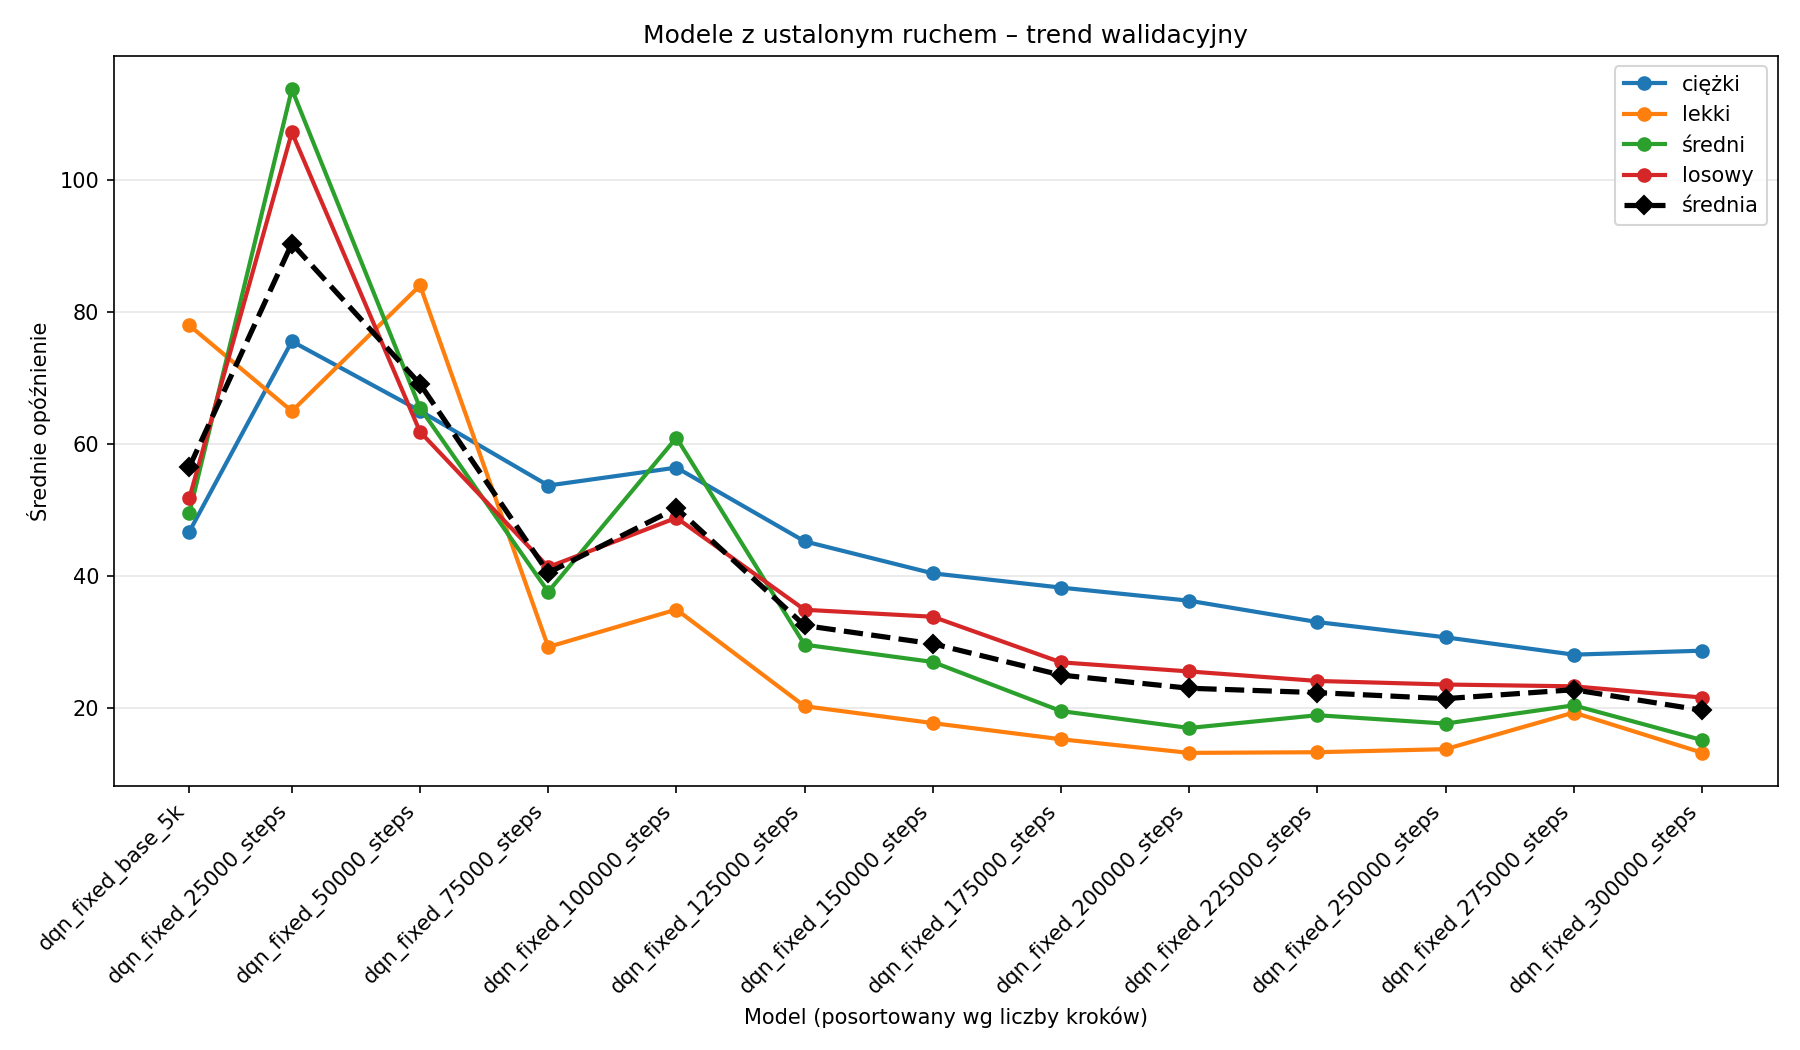
\includegraphics[width=0.9\linewidth]{validate_steps_fixed.png}
    \caption{Średnie opóźnienie kolejnych checkpointów modelu trenowanego na regularnym zbiorze treningowym, w podziale na scenariusze walidacyjne.}
    \label{fig:checkpointy-fixed}
\end{figure}

Przebieg wyników dzieli się na dwie wyraźne części. W pierwszych 100\,000 kroków opóźnienie maleje szybko i we wszystkich scenariuszach jednocześnie, przy czym checkpoint po 50\,000 krokach wypada gorzej niż poprzedni, co odpowiada okresowi intensywnej eksploracji, kończącemu się po 60\,000 kroków. Powyżej 125\,000 kroków wyniki na scenariuszach lekkim, średnim i zmiennym stabilizują się: ich średnia mieści się w przedziale od 23,15 do 27,30, a więc rozstęp wynosi 17\% wartości średniej.

Scenariusz o wysokim natężeniu zachowuje się odmiennie. Nie osiąga on stabilnego poziomu, a po przekroczeniu 125\,000 kroków wartości wahają się od 51,35 do 77,94, co odpowiada rozstępowi rzędu 38\% wartości średniej. Ponieważ bezwzględne wartości opóźnienia są w tym scenariuszu kilkukrotnie wyższe niż w pozostałych, zdominowałyby one średnią z czterech scenariuszy. Z tego powodu na rysunku~\ref{fig:zbiory-treningowe} przedstawiono scenariusze stabilne oraz scenariusz o wysokim natężeniu na osobnych wykresach.

Najniższą średnią z czterech scenariuszy, równą 30,33, uzyskał checkpoint po 225\,000 kroków. Powyżej tej wartości nie zaobserwowano dalszej poprawy: średnia dla checkpointów po 250\,000, 275\,000 oraz 300\,000 kroków wynosi odpowiednio 37,37, 36,33 oraz 36,51, czyli wraca do poziomu sprzed 225\,000 kroków. Wynik na scenariuszu o wysokim natężeniu pogarsza się przy tym z 51,35 do wartości przekraczających 74. Obserwacja ta wskazuje na utratę stabilności procesu uczenia lub na nadmierne dopasowanie do scenariuszy treningowych, przy czym samo porównanie checkpointów nie pozwala rozstrzygnąć między tymi wyjaśnieniami.

Należy zaznaczyć, że przewaga checkpointu po 225\,000 kroków wynika w tabeli~\ref{tab:checkpointy-fixed} niemal wyłącznie z jednego wyniku na scenariuszu o wysokim natężeniu, uzyskanego w pojedynczym przebiegu. Wybór oparty na takiej podstawie byłby zatem niewiarygodny, co stało się przesłanką do powtórzenia oceny na wielu ziarnach, opisanego w podrozdziale~\ref{subsec:wieloziarnowa-checkpointy}.

\subsection{Porównanie wariantów zbioru treningowego}
\label{subsec:porownanie-zbiorow}

Tę samą procedurę powtórzono dla drugiego wariantu zbioru treningowego, opisanego w podrozdziale~\ref{subsubsec:trening-nieregularny}, w którym czasy wyjazdu pojazdów rozmieszczone są nieregularnie, a średnie natężenie różni się między scenariuszami tego samego poziomu obciążenia. Konfiguracja algorytmu, długość treningu oraz sposób oceny pozostały niezmienione, dzięki czemu jedyną różnicą między obiema seriami jest sposób generowania danych treningowych.

Zestawienie obu wariantów przedstawiono w tabeli~\ref{tab:zbiory-treningowe}, a przebieg wyników na rysunku~\ref{fig:zbiory-treningowe}.

\begin{table}[!htbp] \centering
    \caption{Porównanie wariantów zbioru treningowego. Wartości uśrednione po dwunastu checkpointach, w nawiasie odchylenie standardowe.}
    \label{tab:zbiory-treningowe}
    \small
    \begin{tabular}{| l | r | r | r | r |} \hline
        Zbiór treningowy & Lekki & Średni & Wysoki & Zmienny \\ \hline\hline
        regularny    & 21,70 (13,98) & 25,71 (11,14) & 71,42 (10,00) & 42,55 (6,97) \\ \hline
        nieregularny & 31,56 (35,45) & 28,96 (20,61) & 91,26 (12,26) & 53,23 (17,72) \\ \hline
    \end{tabular}
\end{table}

\begin{figure}[!htbp] \centering
    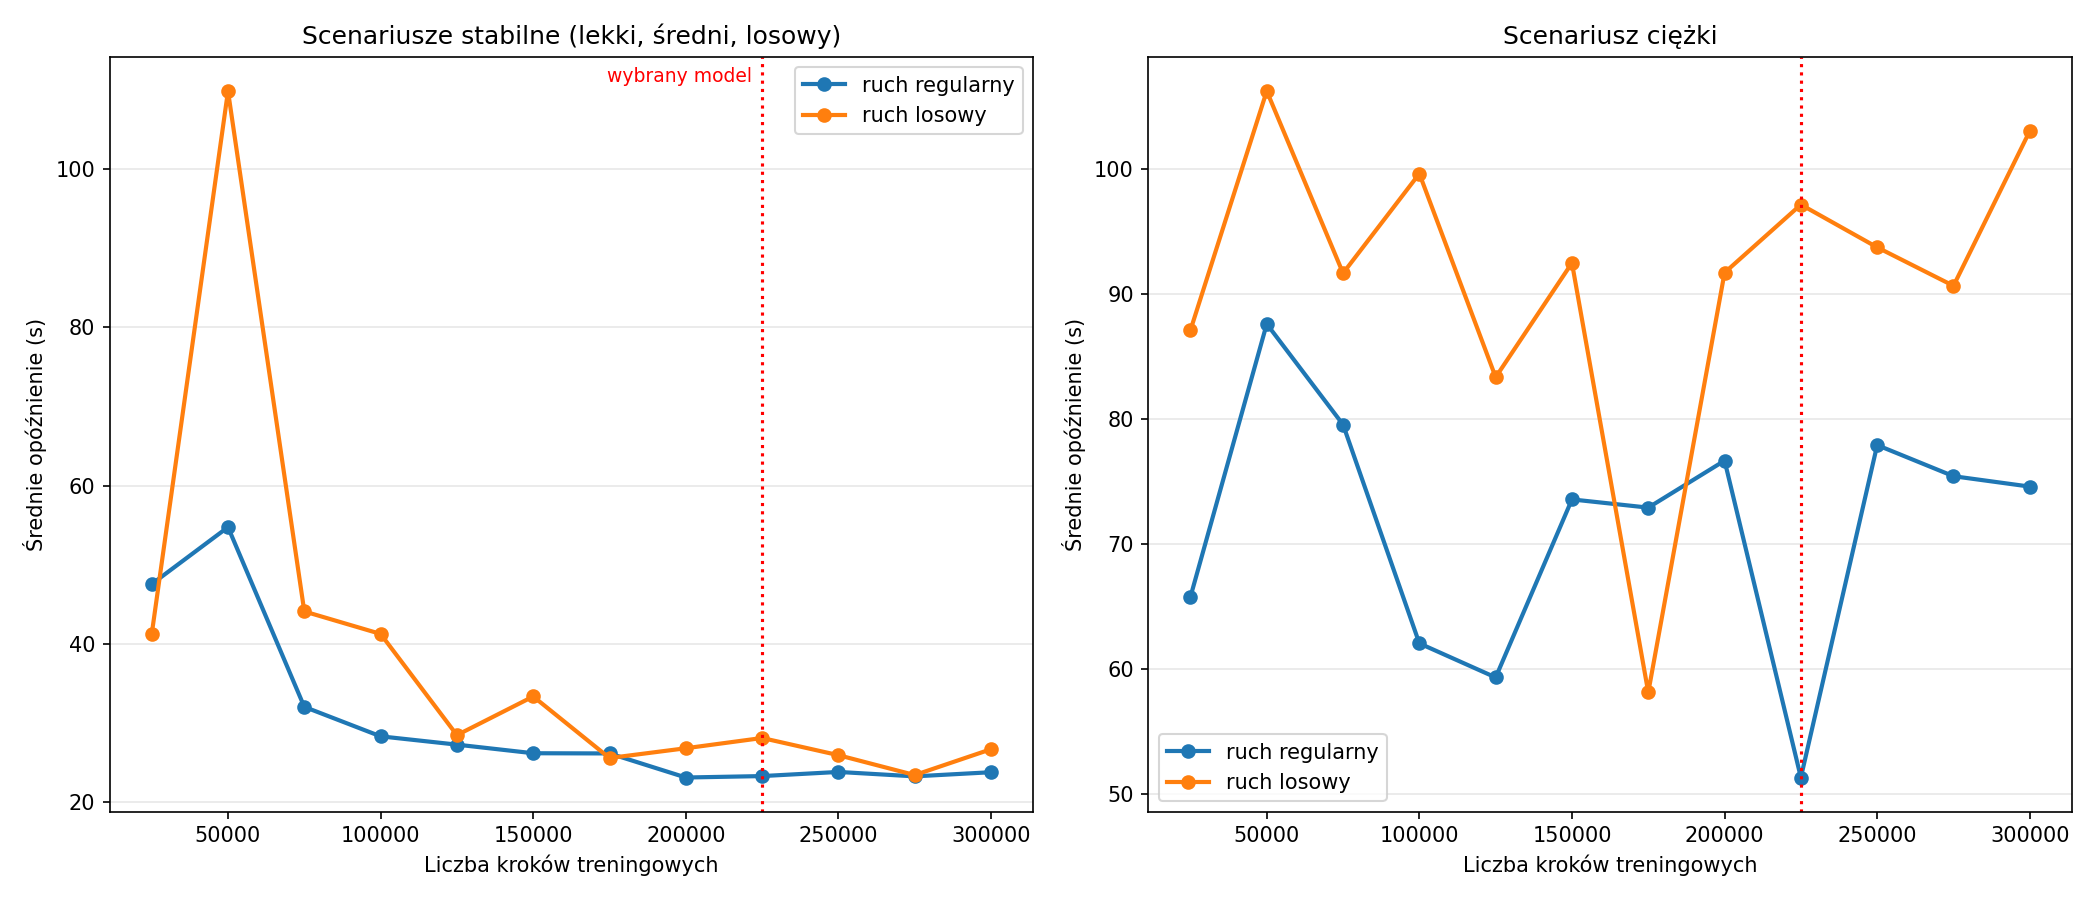
\includegraphics[width=\linewidth]{validate_steps_stabilne_vs_ciezki.png}
    \caption{Porównanie wariantów zbioru treningowego na scenariuszach stabilnych oraz na scenariuszu o wysokim natężeniu.}
    \label{fig:zbiory-treningowe}
\end{figure}

Model trenowany na regularnym zbiorze treningowym okazał się lepszy w każdym z czterech scenariuszy walidacyjnych. Największa różnica dotyczy scenariusza o wysokim natężeniu, gdzie średnia po wszystkich checkpointach wynosi 71,42 wobec 91,26, czyli o 27,8\% więcej dla wariantu nieregularnego. Po przekroczeniu 125\,000 kroków rozstęp wyników na tym scenariuszu wynosi 38\% wartości średniej dla zbioru regularnego oraz 51\% dla nieregularnego. Także na scenariuszach stabilnych rozstęp jest ponad dwukrotnie większy dla wariantu nieregularnego, co odpowiada wyraźnie większym odchyleniom standardowym w tabeli~\ref{tab:zbiory-treningowe}.

Na uwagę zasługuje wynik na scenariuszu o zmiennym natężeniu, czyli tym, który sam został wygenerowany z nieregularnym rozmieszczeniem czasów wyjazdu. Również w nim lepszy okazał się model trenowany na danych regularnych: 42,55 wobec 53,23. Większa losowość danych treningowych nie przełożyła się zatem na lepsze działanie na scenariuszu o zbliżonej charakterystyce. Obserwacja ta dotyczy wyłącznie badanej konfiguracji i nie stanowi ogólnej zasady, a jej możliwe wyjaśnienia omówiono w rozdziale~\ref{sec:analiza}.

Na podstawie tego porównania do dalszych etapów badania wybrano regularny zbiór treningowy. Wszystkie warianty strojenia hiperparametrów trenowano już wyłącznie na tym zbiorze.

\subsection{Weryfikacja wyboru checkpointu na wielu ziarnach}
\label{subsec:wieloziarnowa-checkpointy}

Ponieważ pojedynczy przebieg walidacyjny okazał się niewystarczającą podstawą wyboru, trzech kandydatów oceniono ponownie na pięciu ziarnach symulacji. Wybrano checkpoint po 225\,000 kroków jako najlepszy w ocenie jednoprzebiegowej oraz dwa checkpointy sąsiednie w rankingu, to jest po 200\,000 oraz po 275\,000 kroków. Wyniki przedstawiono w tabeli~\ref{tab:checkpointy-ziarna} oraz na rysunku~\ref{fig:checkpointy-ziarna}.

\begin{table}[!htbp] \centering
    \caption{Walidacja kandydatów na model końcowy na pięciu ziarnach symulacji. W nawiasie odchylenie standardowe.}
    \label{tab:checkpointy-ziarna}
    \small
    \begin{tabular}{| r | r | r | r | r | r |} \hline
        Kroki & Lekki & Średni & Wysoki & Zmienny & Średnia \\ \hline\hline
        200\,000 & 14,65 (0,25) & 21,03 (1,07) & 68,98 (4,50) & 36,58 (1,41) & 35,31 \\ \hline
        \textbf{225\,000} & \textbf{13,94} (0,18) & \textbf{18,78} (0,29) & \textbf{58,76} (5,08) & \textbf{35,48} (1,65) & \textbf{31,74} \\ \hline
        275\,000 & 14,61 (0,27) & 18,74 (0,40) & 72,89 (2,74) & 37,00 (1,72) & 35,81 \\ \hline
    \end{tabular}
\end{table}

\begin{figure}[!htbp] \centering
    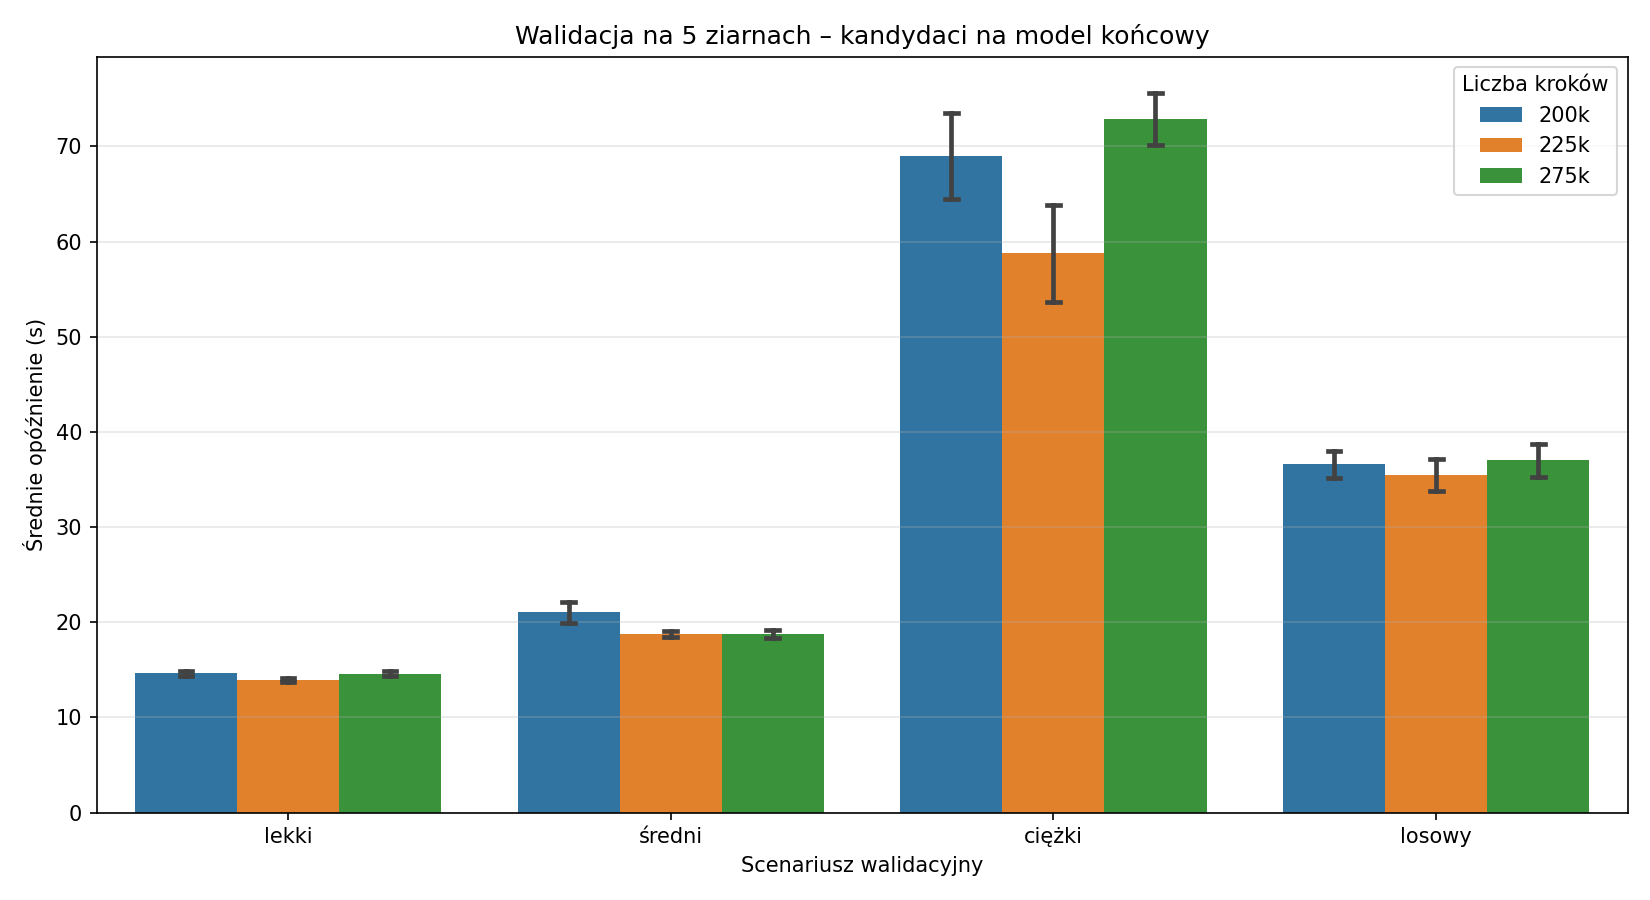
\includegraphics[width=0.85\linewidth]{validate_steps_wieloziarnowa.png}
    \caption{Walidacja trzech kandydatów na model końcowy na pięciu ziarnach symulacji.}
    \label{fig:checkpointy-ziarna}
\end{figure}

Powtórzenie oceny potwierdziło wybór, jednocześnie korygując skalę przewagi. Wynik checkpointu po 225\,000 kroków na scenariuszu o wysokim natężeniu wzrósł z 51,35 w pojedynczym przebiegu do 58,76 przy uśrednieniu po pięciu ziarnach, co potwierdza, że pojedyncza ocena była nadmiernie optymistyczna. Model ten pozostaje jednak najlepszy w trzech z czterech scenariuszy oraz w średniej z czterech scenariuszy, gdzie uzyskuje 31,74 wobec 35,31 i 35,81 dla pozostałych kandydatów.

Odchylenia standardowe pokazują wyraźną różnicę między scenariuszami. Na scenariuszach lekkim i średnim wynoszą one poniżej 1,1, natomiast na scenariuszu o wysokim natężeniu sięgają 5,08. Przy wysokim natężeniu ruchu różnice wynikające ze zmiany ziarna symulacji są podobnej wielkości jak różnice między modelami. Dlatego na dalszych etapach modele oceniano na wielu ziarnach.

\subsection{Dobór hiperparametrów}
\label{subsec:strojenie}

\subsubsection{Plan eksperymentu}
\label{subsubsec:plan-strojenia}

Strojenie prowadzono metodą zmiany jednego hiperparametru. Pozostałe wartości pozostawiano bez zmian. Punktem odniesienia była konfiguracja bazowa z tabeli~\ref{tab:konfiguracja-bazowa}. Każdy wariant trenowano na regularnym zbiorze treningowym przez 225\,000 kroków, czyli dokładnie tyle, ile liczy wybrany checkpoint modelu bazowego, dzięki czemu porównanie nie jest zaburzone różną długością treningu. Ziarno algorytmu oraz procedura walidacji pozostały niezmienione.

Przebadano dwanaście wariantów zmieniających pojedynczy hiperparametr, przy czym dla czterech z nich sprawdzono obie strony wartości bazowej, oraz cztery warianty dodatkowe, w tym dwa łączące zmiany kilku parametrów jednocześnie i jeden zmieniający architekturę sieci. Zakres zmian obejmował tempo uczenia, rozmiar batcha, pojemność bufora doświadczeń, współczynnik dyskontowania, długość fazy eksploracji, częstotliwość aktualizacji sieci docelowej, częstotliwość aktualizacji gradientowych, próg rozpoczęcia uczenia oraz układ warstw ukrytych.

\subsubsection{Wyniki poszczególnych wariantów}
\label{subsubsec:wyniki-strojenia}

Wyniki wszystkich wariantów zestawiono w tabeli~\ref{tab:strojenie}, uporządkowane rosnąco według średniej z czterech scenariuszy walidacyjnych. Odpowiadające im wykresy przedstawiono na rysunku~\ref{fig:strojenie}, gdzie górny panel obrazuje średnią, a dolny rozbicie na poszczególne scenariusze.

\begin{table}[!htbp] \centering
    \caption{Wyniki strojenia hiperparametrów na zbiorze walidacyjnym. Średnie opóźnienie w sekundach, pojedynczy przebieg na scenariusz.}
    \label{tab:strojenie}
    \footnotesize
    \setlength{\tabcolsep}{4pt}
    \begin{tabular}{| l | l | r | r | r | r | r |} \hline
        Wariant & Zmiana względem konfiguracji bazowej & Lekki & Średni & Wysoki & Zmienny & Średnia \\ \hline\hline
        \textbf{bazowy} & \textbf{brak} & \textbf{13,87} & \textbf{19,48} & \textbf{51,35} & \textbf{36,63} & \textbf{30,33} \\ \hline
        \texttt{tui250}       & \texttt{target\_update\_interval} 250   & 15,16 & 19,86 & 69,34 & 36,94 & 35,32 \\ \hline
        \texttt{batch32}      & \texttt{batch\_size} 32                 & 14,79 & 18,61 & 75,81 & 32,48 & 35,43 \\ \hline
        \texttt{trainfreq4}   & \texttt{train\_freq} 4                  & 15,23 & 19,41 & 74,28 & 34,66 & 35,89 \\ \hline
        \texttt{tui1e3}       & \texttt{target\_update\_interval} 1000  & 15,82 & 21,32 & 69,09 & 38,37 & 36,15 \\ \hline
        \texttt{lr3e-4}       & \texttt{learning\_rate} 0,0003          & 13,50 & 18,25 & 76,55 & 37,74 & 36,51 \\ \hline
        \texttt{lr3e-4+gam98} & \texttt{learning\_rate} 0,0003 i \texttt{gamma} 0,98 & 13,40 & 18,68 & 80,94 & 34,34 & 36,84 \\ \hline
        \texttt{batch128}     & \texttt{batch\_size} 128                & 15,18 & 18,79 & 76,88 & 36,76 & 36,90 \\ \hline
        \texttt{net128}       & warstwy ukryte [128, 128]               & 16,11 & 22,69 & 71,27 & 42,11 & 38,05 \\ \hline
        \texttt{lr3e-4+bat32} & \texttt{learning\_rate} 0,0003 i \texttt{batch\_size} 32 & 13,68 & 17,92 & 82,54 & 40,18 & 38,58 \\ \hline
        \texttt{explore3e-1}  & \texttt{exploration\_fraction} 0,3      & 13,93 & 18,53 & 74,77 & 49,12 & 39,09 \\ \hline
        \texttt{gamma98e-2}   & \texttt{gamma} 0,98                     & 13,90 & 18,77 & 80,94 & 43,70 & 39,33 \\ \hline
        \texttt{lr5e-4}       & \texttt{learning\_rate} 0,0005          & 14,68 & 18,38 & 82,31 & 44,29 & 39,91 \\ \hline
        \texttt{starts5e3}    & \texttt{learning\_starts} 5000          & 15,35 & 19,99 & 84,45 & 40,25 & 40,01 \\ \hline
        \texttt{buffer1e5}    & \texttt{buffer\_size} 100\,000          & 17,27 & 20,44 & 84,91 & 42,06 & 41,17 \\ \hline
        \texttt{gamma995e-3}  & \texttt{gamma} 0,995                    & 14,96 & 19,98 & 89,65 & 40,54 & 41,28 \\ \hline
        \texttt{explore1e-1}  & \texttt{exploration\_fraction} 0,1      & 15,48 & 20,72 & 104,92 & 65,69 & 51,70 \\ \hline
    \end{tabular}
\end{table}

\begin{figure}[!htbp] \centering
    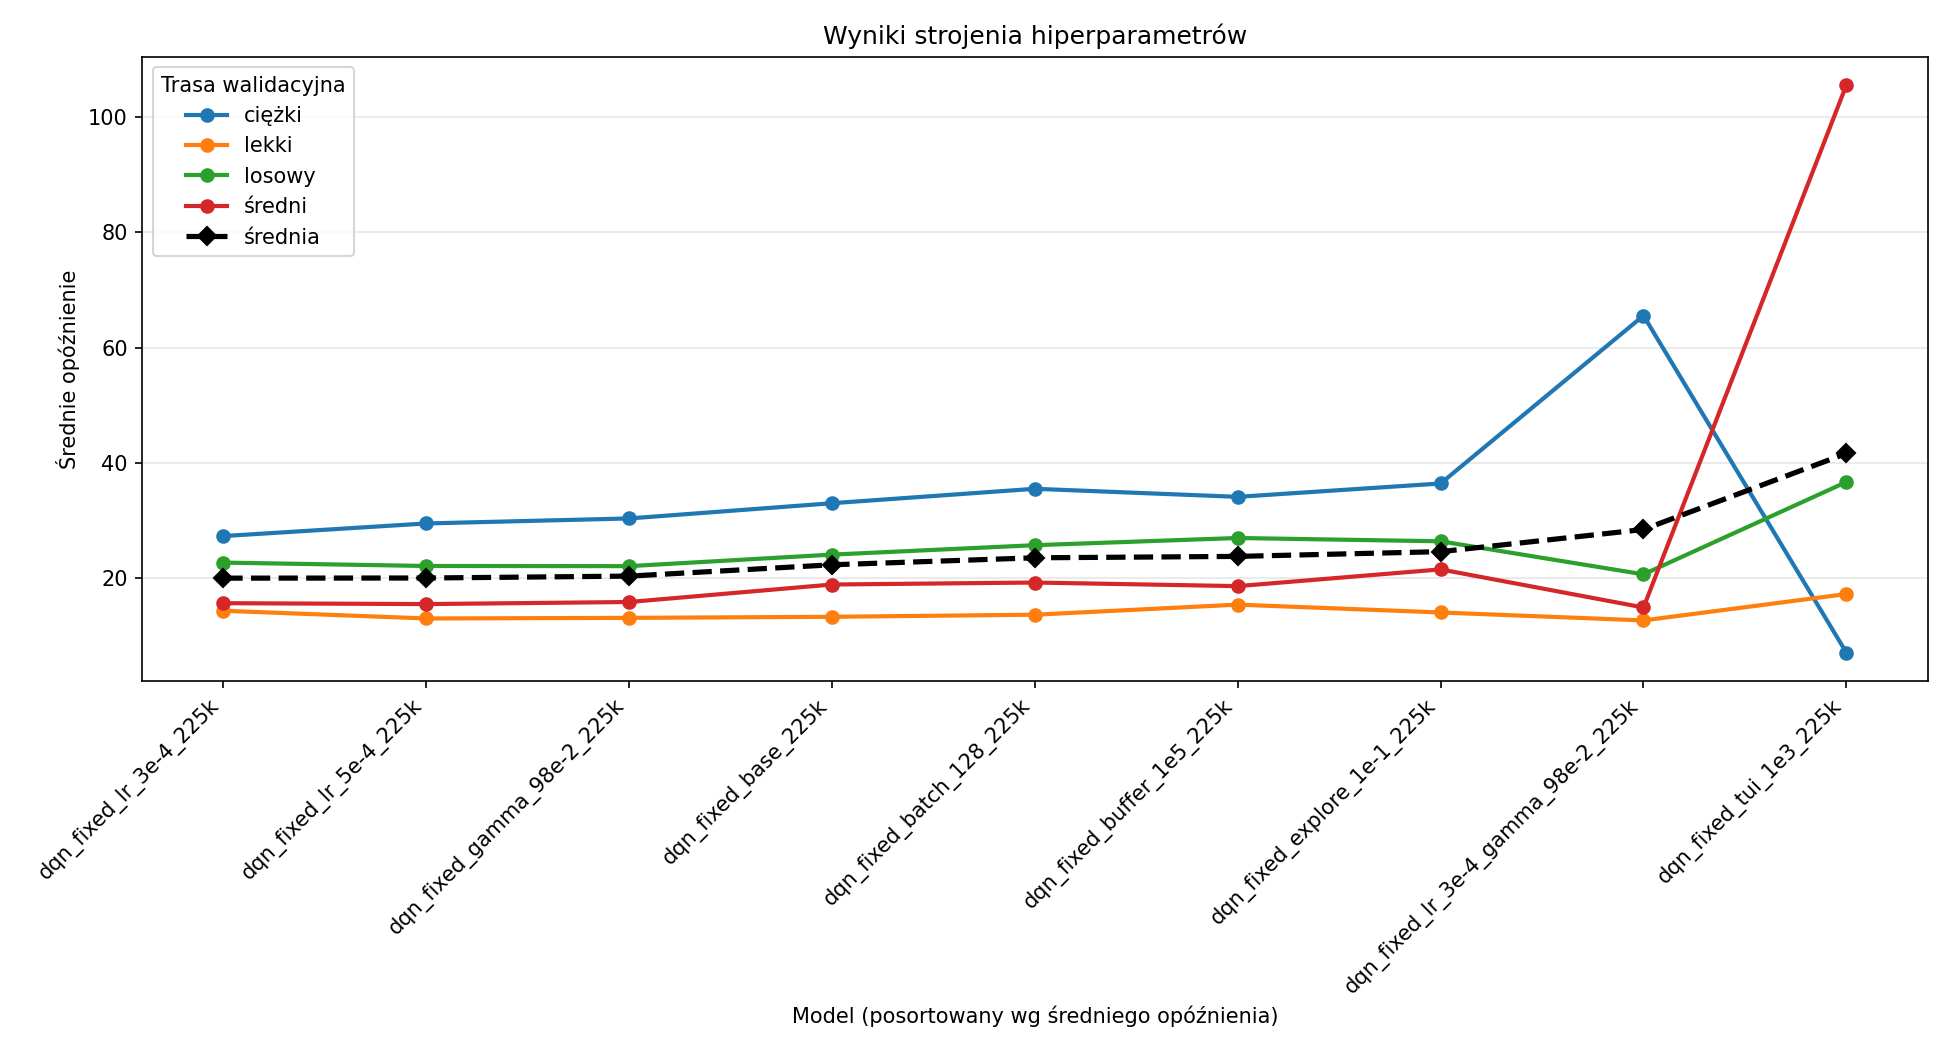
\includegraphics[width=\linewidth]{hyperparameter_tuning.png}
    \caption{Wyniki strojenia hiperparametrów: średnia z czterech scenariuszy oraz rozbicie na poszczególne scenariusze.}
    \label{fig:strojenie}
\end{figure}

Żaden z szesnastu badanych wariantów nie poprawił średniej z czterech scenariuszy względem konfiguracji bazowej. Najlepszy z nich uzyskał 35,32 wobec 30,33, a najgorszy 51,70.

Dla czterech hiperparametrów sprawdzono zmianę w obie strony i w każdym z tych przypadków wartość bazowa okazała się lepsza od obu wartości sąsiednich. Częstotliwość aktualizacji sieci docelowej dała 35,32 dla wartości 250 oraz 36,15 dla wartości 1000, przy 30,33 dla wartości 500. Współczynnik dyskontowania dał 39,33 dla 0,98 oraz 41,28 dla 0,995. Rozmiar batcha dał 35,43 dla 32 oraz 36,90 dla 128. Długość fazy eksploracji dała 51,70 dla 0,1 oraz 39,09 dla 0,3.

Najsilniejszy wpływ na wynik miała długość fazy eksploracji. Skrócenie jej z 0,2 do 0,1 pogorszyło średnią o 70,5\%, przy czym pogorszenie dotyczy przede wszystkim scenariuszy o wysokim i zmiennym natężeniu, gdzie opóźnienie wzrosło odpowiednio z 51,35 do 104,92 oraz z 36,63 do 65,69. Wariant ten wybrano następnie jako model kontrastowy do oceny na zbiorze testowym, co opisano w podrozdziale~\ref{subsec:model-kontrastowy}.

Rozbicie na scenariusze, widoczne w dolnej części rysunku~\ref{fig:strojenie}, pokazuje, że sama średnia nie opisuje zachowania wariantów w pełni. Część z nich wypada lepiej od konfiguracji bazowej w wybranych scenariuszach: obniżenie tempa uczenia do 0,0003 daje najniższe opóźnienie na scenariuszu lekkim, jego połączenie ze zmniejszonym rozmiarem batcha na scenariuszu średnim, a samo zmniejszenie rozmiaru batcha do 32 na scenariuszu zmiennym, gdzie daje 32,48 wobec 36,63. Żaden wariant nie okazał się natomiast lepszy od konfiguracji bazowej na scenariuszu o wysokim natężeniu, gdzie najlepszy wynik wśród wariantów wynosi 69,09 wobec 51,35. Ponieważ bezwzględne wartości opóźnienia są w tym scenariuszu największe, to właśnie on decyduje o kolejności w rankingu opartym na średniej.

\subsubsection{Warianty łączące zmiany kilku hiperparametrów}
\label{subsubsec:warianty-laczone}

Dodatkowo sprawdzono, czy zmiany korzystne w pojedynczych scenariuszach przynoszą poprawę po połączeniu. Zbadano dwie kombinacje wywodzące się z obniżonego tempa uczenia, które w ocenie jednoparametrowej dawało najlepsze wyniki na scenariuszach lekkim i średnim.

Połączenie tempa uczenia 0,0003 ze współczynnikiem dyskontowania 0,98 dało średnią 36,84, czyli wynik lepszy niż sam zmieniony współczynnik dyskontowania, wynoszący 39,33, lecz gorszy niż samo zmienione tempo uczenia, wynoszące 36,51. Połączenie tempa uczenia 0,0003 z rozmiarem batcha 32 dało 38,58, a więc wynik gorszy od obu zmian rozpatrywanych osobno, to jest 36,51 oraz 35,43. W obu kombinacjach pogorszenie dotyczy scenariusza o wysokim natężeniu, gdzie opóźnienie wzrosło do 80,94 oraz 82,54.

Żadna z kombinacji nie poprawiła wyniku względem konfiguracji bazowej ani względem zmian składowych, dlatego obie odrzucono.

\subsubsection{Weryfikacja najlepszych wariantów na wielu ziarnach}
\label{subsubsec:strojenie-ziarna}

Ranking z tabeli~\ref{tab:strojenie} opiera się na pojedynczym przebiegu na scenariusz, podczas gdy konfiguracja bazowa była już oceniona na pięciu ziarnach. Aby porównanie było symetryczne, trzy najlepsze warianty poddano ocenie w takiej samej procedurze wieloziarnowej. Wyniki przedstawiono w tabeli~\ref{tab:strojenie-ziarna} oraz na rysunku~\ref{fig:strojenie-ziarna}.

\begin{table}[!htbp] \centering
    \caption{Porównanie trzech najlepszych wariantów z konfiguracją bazową na pięciu ziarnach symulacji. W nawiasie odchylenie standardowe.}
    \label{tab:strojenie-ziarna}
    \small
    \begin{tabular}{| l | r | r | r | r | r |} \hline
        Konfiguracja & Lekki & Średni & Wysoki & Zmienny & Średnia \\ \hline\hline
        \textbf{bazowa} & \textbf{13,94} (0,18) & 18,78 (0,29) & \textbf{58,76} (5,08) & 35,48 (1,65) & \textbf{31,74} \\ \hline
        \texttt{batch32}    & 14,64 (0,46) & \textbf{18,65} (0,42) & 77,89 (0,92) & \textbf{32,58} (1,67) & 35,94 \\ \hline
        \texttt{tui250}     & 15,51 (0,47) & 20,15 (0,36) & 72,92 (3,09) & 37,28 (2,15) & 36,46 \\ \hline
        \texttt{trainfreq4} & 15,66 (0,36) & 19,45 (0,21) & 78,97 (6,39) & 35,13 (2,11) & 37,31 \\ \hline
    \end{tabular}
\end{table}

\begin{figure}[!htbp] \centering
    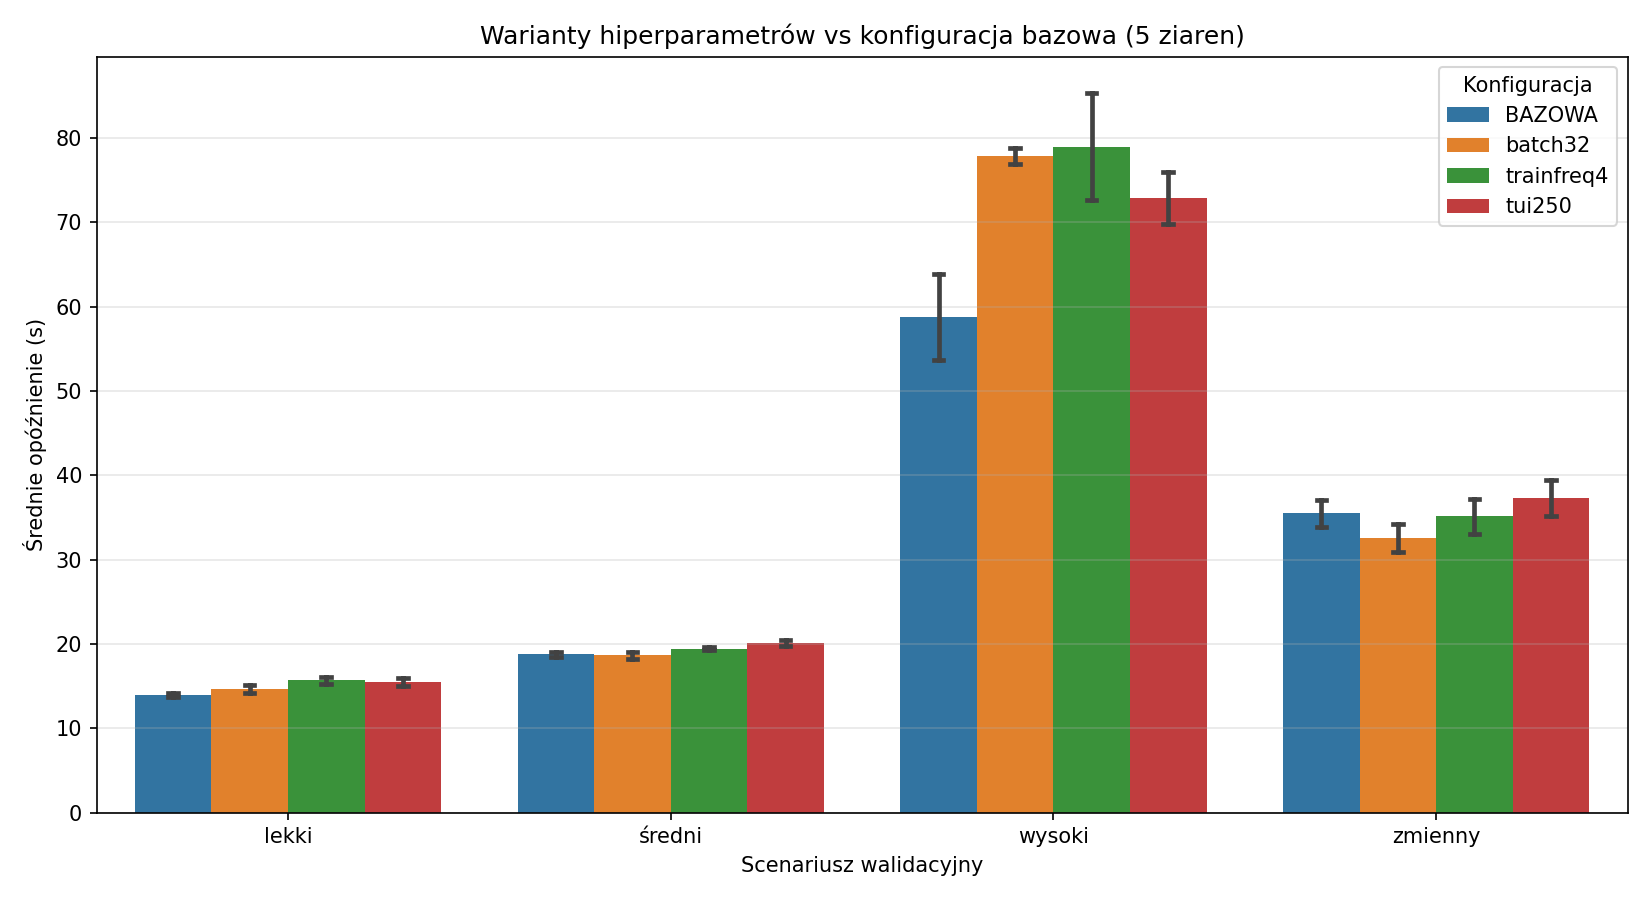
\includegraphics[width=0.85\linewidth]{hyperparameter_wieloziarnowa.png}
    \caption{Trzy najlepsze warianty hiperparametrów w porównaniu z konfiguracją bazową, ocena na pięciu ziarnach symulacji.}
    \label{fig:strojenie-ziarna}
\end{figure}

Konfiguracja bazowa zachowała przewagę w ocenie wieloziarnowej. Jej średnia wyniosła 31,74, a dla pozostałych wariantów odpowiednio 35,94, 36,46 i 37,31. Uzyskała również najniższe opóźnienie na scenariuszach lekkim i o wysokim natężeniu. W drugim z nich różnica była największa i wyniosła od 14,16 do 20,21 sekundy na pojazd.

Jedyną przewagą wariantu nad konfiguracją bazową, która utrzymała się po uśrednieniu po pięciu ziarnach, jest wynik wariantu ze zmniejszonym rozmiarem batcha na scenariuszu o zmiennym natężeniu, wynoszący 32,58 wobec 35,48, oraz nieznacznie niższy wynik tego samego wariantu na scenariuszu średnim. Wariant ten traci jednak 19,13 sekundy na scenariuszu o wysokim natężeniu.

\subsection{Wybór modelu końcowego}
\label{subsec:model-koncowy}

Na podstawie wyników walidacyjnych jako model końcowy przyjęto konfigurację bazową wytrenowaną na regularnym zbiorze treningowym, w stanie po 225\,000 kroków. Odpowiada jej plik \texttt{dqn\_fixed\_225000\_steps.zip}, którego kopia zapisana jest jako model końcowy. Pełny zestaw hiperparametrów tej konfiguracji przedstawiono w tabeli~\ref{tab:konfiguracja-bazowa}.

Za wyborem przemawiały trzy przesłanki wynikające z wcześniejszych podrozdziałów. Po pierwsze, regularny zbiór treningowy dał lepsze wyniki niż nieregularny we wszystkich czterech scenariuszach walidacyjnych. Po drugie, punkt po 225\,000 kroków uzyskał najniższe średnie opóźnienie zarówno w ocenie kolejnych checkpointów, jak i w powtórzonej ocenie na pięciu ziarnach, a dalsze wydłużanie treningu nie przynosiło poprawy. Po trzecie, żaden z szesnastu badanych wariantów hiperparametrów nie poprawił wyniku, a trzy najlepsze z nich pozostały gorsze także po ocenie wieloziarnowej.

Konfigurację modelu końcowego zamrożono przed pierwszym uruchomieniem ewaluacji testowej i nie zmieniano jej po zapoznaniu się z wynikami.

\subsection{Końcowe porównanie metod na zbiorze testowym}
\label{subsec:wyniki-testowe}

\subsubsection{Przebieg oceny}
\label{subsubsec:przebieg-oceny-testowej}

Model końcowy oceniono na wszystkich dwudziestu scenariuszach testowych, przy tych samych plikach tras i tych samych ziarnach symulacji, których użyto wcześniej dla metod referencyjnych. Wyniki przedstawiane są jako średnia z pięciu scenariuszy danego poziomu natężenia wraz z odchyleniem standardowym.

Podczas oceny ujawniła się różnica w sposobie kończenia przebiegu. Przebiegi metod referencyjnych kończyły się naturalnie, po obsłużeniu wszystkich pojazdów, w czasie od 3646 do 4454~s symulacji. Trzy z dwudziestu przebiegów agenta DQN osiągnęły natomiast zabezpieczający limit czasu symulacji, wynoszący 20\,000~s, ponieważ pozostała w sieci niewielka grupa pojazdów, która nie opuściła skrzyżowania. Dotyczy to jednego scenariusza o wysokim natężeniu, w którym obsłużonych zostało 2872 z 2880 podróży, oraz dwóch scenariuszy o zmiennym natężeniu, w których obsłużono odpowiednio 1693 z 1705 oraz 1608 z 1623 podróży. Udział pojazdów nieobsłużonych nie przekracza zatem 1\% w żadnym z tych przebiegów.

Zjawisko to ma znaczenie dla odczytu wyników, ponieważ część metryk normowana jest czasem trwania symulacji. Wpływ ten oszacowano przez porównanie wartości wyznaczonych ze wszystkich przebiegów z wartościami wyznaczonymi wyłącznie z przebiegów zakończonych naturalnie, co zestawiono w tabeli~\ref{tab:blokady}.

\begin{table}[!htbp] \centering
    \caption{Wpływ przebiegów zakończonych limitem czasu na wyniki agenta DQN.}
    \label{tab:blokady}
    \footnotesize
    \setlength{\tabcolsep}{3pt}
    \begin{tabular}{| l | l | r | r |} \hline
        Metryka & Scenariusz & Wszystkie przebiegi & Bez przebiegów przerwanych limitem \\ \hline\hline
        średnie opóźnienie [s]      & wysoki  & 51,82   & 51,97 \\ \hline
        średnie opóźnienie [s]      & zmienny & 34,23   & 34,69 \\ \hline
        średni czas oczekiwania [s] & wysoki  & 28,90   & 28,98 \\ \hline
        średni czas oczekiwania [s] & zmienny & 17,27   & 17,51 \\ \hline
        średnia długość kolejki [poj.] & wysoki  & 18,04   & 19,96 \\ \hline
        średnia długość kolejki [poj.] & zmienny & 9,55    & 7,63 \\ \hline
        przepustowość [poj./h]      & wysoki  & 2700,90 & 2690,32 \\ \hline
        przepustowość [poj./h]      & zmienny & 1594,49 & 1591,48 \\ \hline
        częstotliwość przełączeń [1/h] & wysoki  & 232,85  & 278,10 \\ \hline
        częstotliwość przełączeń [1/h] & zmienny & 193,94  & 286,69 \\ \hline
    \end{tabular}
\end{table}

Metryki wyznaczane z pliku \texttt{tripinfo.xml}, to jest średnie opóźnienie oraz średni czas oczekiwania, pozostają praktycznie niezmienione, ponieważ dotyczą zakończonych podróży, a udział podróży niezakończonych jest znikomy. Wyraźnie zmieniają się natomiast metryki normowane czasem, przede wszystkim częstotliwość przełączeń. W dalszej części podrozdziału podawane są wartości wyznaczone ze wszystkich przebiegów, a przy metrykach wrażliwych na to zjawisko przywoływana jest dodatkowo wartość skorygowana.

\subsubsection{Średnie opóźnienie}
\label{subsubsec:test-opoznienie}

Wartości średniego opóźnienia zestawiono w tabeli~\ref{tab:test-opoznienie}, a ich rozkład przedstawiono na rysunkach~\ref{fig:test-opoznienie} oraz~\ref{fig:test-opoznienie-box}.

\begin{table}[!htbp] \centering
    \caption{Średnie opóźnienie na zbiorze testowym w sekundach na pojazd. W nawiasie odchylenie standardowe.}
    \label{tab:test-opoznienie}
    \small
    \begin{tabular}{| l | r | r | r | r |} \hline
        Metoda & Lekki & Średni & Wysoki & Zmienny \\ \hline\hline
        stałoczasowa & 28,00 (0,81) & 30,91 (0,56) & 65,45 (3,83) & 48,25 (3,69) \\ \hline
        akomodacyjna & 15,22 (0,46) & 18,02 (0,47) & 78,07 (6,87) & 39,76 (6,98) \\ \hline
        \textbf{DQN} & \textbf{13,90} (0,58) & \textbf{17,79} (0,42) & \textbf{51,82} (6,95) & \textbf{34,23} (5,36) \\ \hline
    \end{tabular}
\end{table}

\begin{figure}[!htbp] \centering
    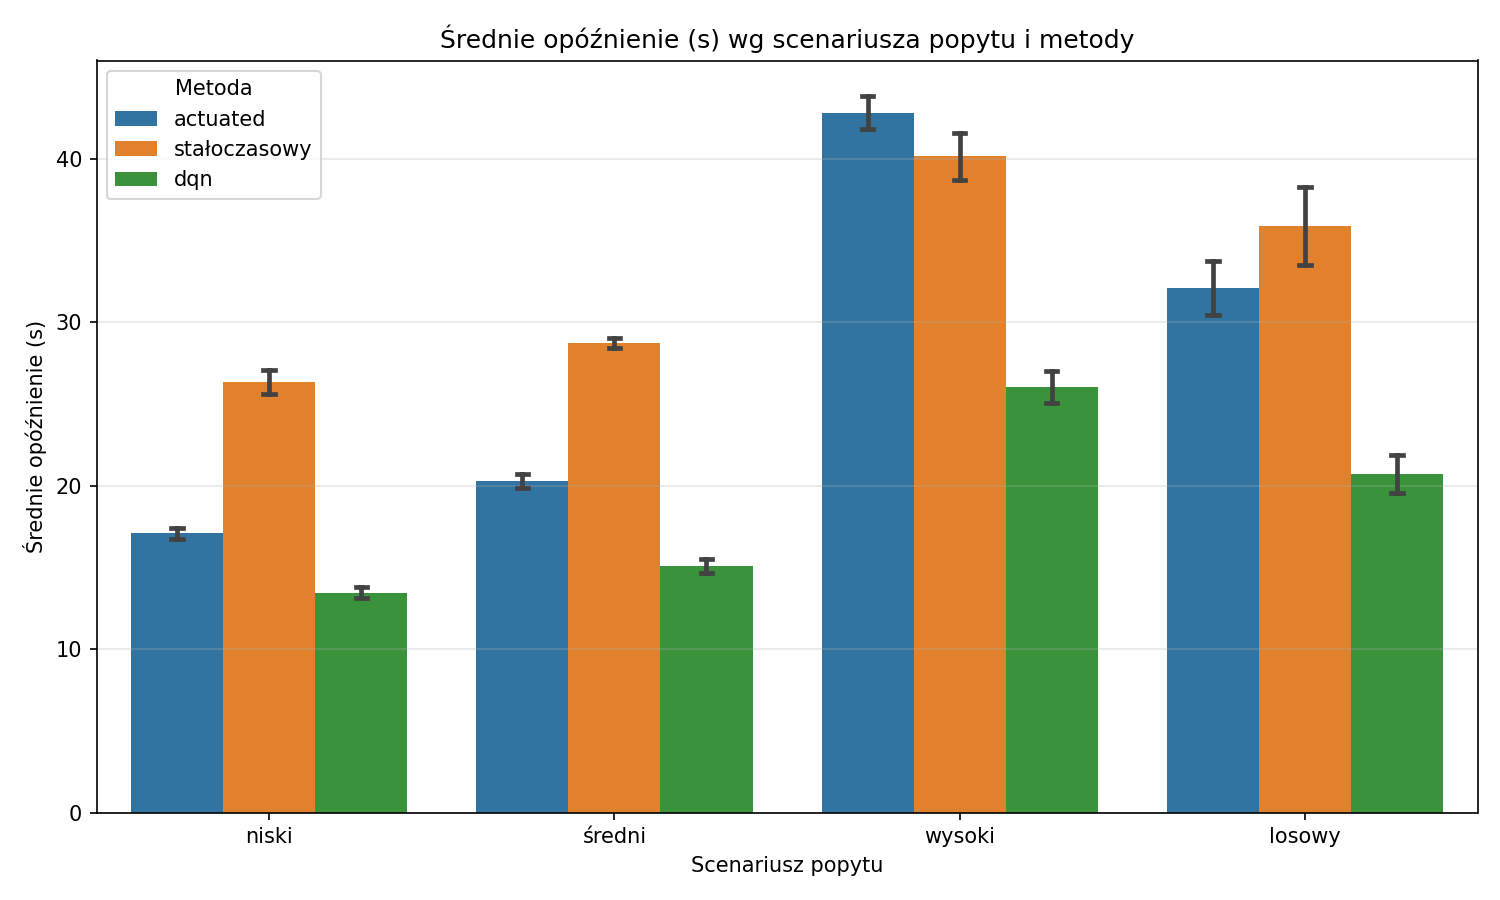
\includegraphics[width=0.8\linewidth]{results_bar_mean_delay_simp.png}
    \caption{Średnie opóźnienie według scenariusza natężenia oraz metody sterowania.}
    \label{fig:test-opoznienie}
\end{figure}

\begin{figure}[!htbp] \centering
    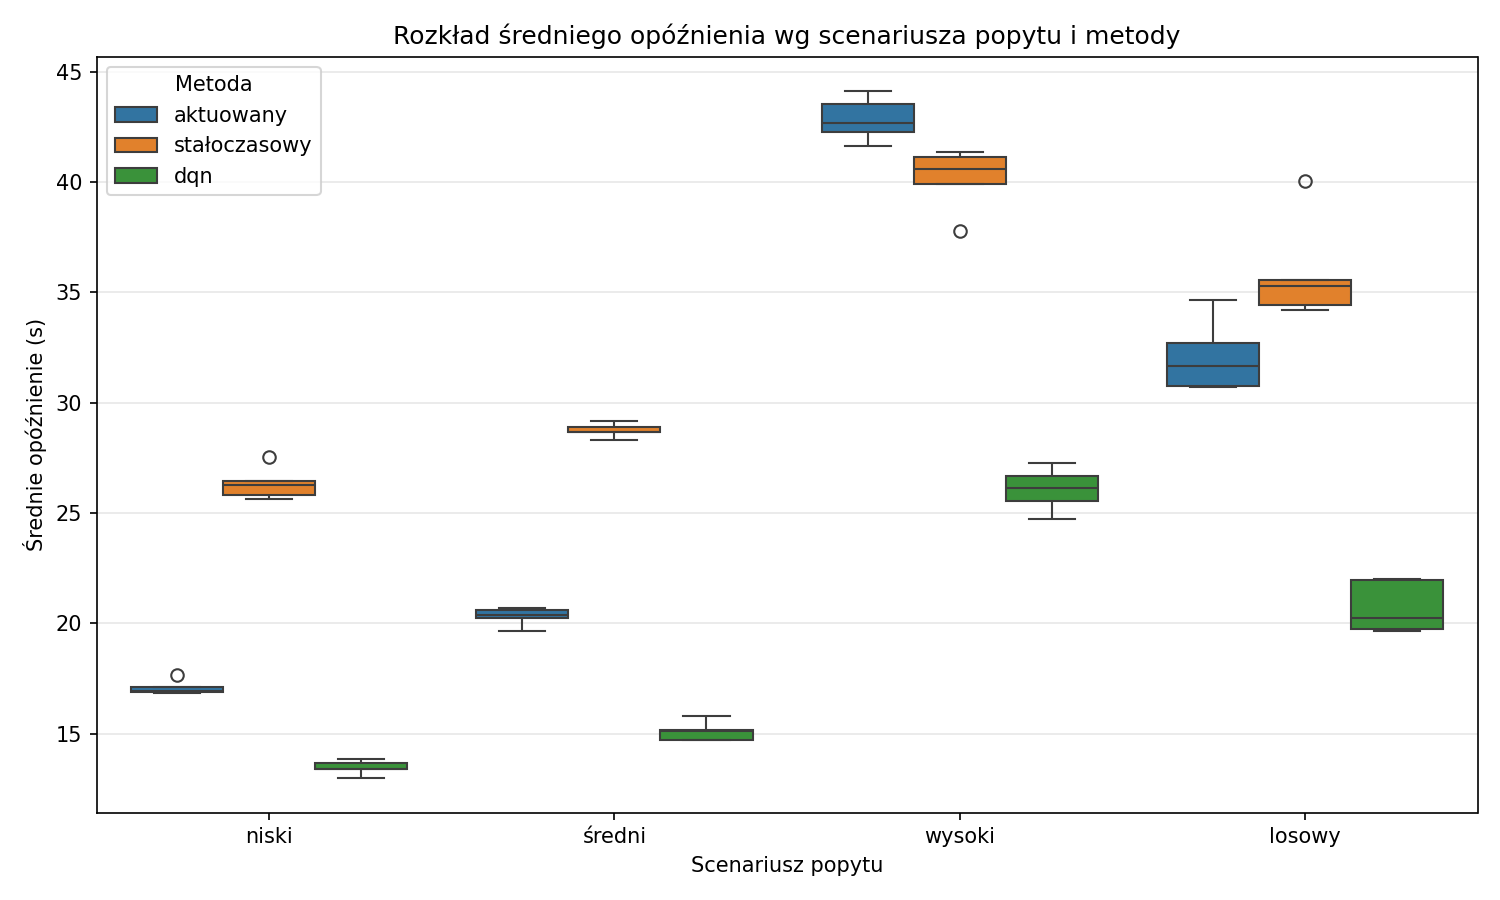
\includegraphics[width=0.8\linewidth]{results_boxplot_mean_delay_simp.png}
    \caption{Rozkład średniego opóźnienia według scenariusza natężenia oraz metody sterowania.}
    \label{fig:test-opoznienie-box}
\end{figure}

Agent DQN uzyskał najniższe średnie opóźnienie we wszystkich czterech scenariuszach. Względem programu stałoczasowego różnica wynosi od 20,8\% w ruchu wysokim do 50,4\% w ruchu lekkim. Względem programu akomodacyjnego jest ona wyraźnie mniejsza w ruchu lekkim i średnim, gdzie wynosi odpowiednio 8,7\% oraz 1,3\%, a największa w ruchu wysokim, gdzie sięga 33,6\%. W scenariuszu o zmiennym natężeniu różnica względem programu akomodacyjnego wynosi 13,9\%.

Rozkład wyników pokazuje, że przewaga w ruchu lekkim i średnim jest systematyczna: wszystkie pięć przebiegów agenta wypada tam lepiej od programu stałoczasowego, a odchylenia standardowe nie przekraczają 0,6. W ruchu wysokim oraz w ruchu zmiennym rozrzut jest znacznie większy dla wszystkich metod. Odchylenie standardowe agenta wynosi tam 6,95 oraz 5,36, a więc jest zbliżone do odchylenia programu akomodacyjnego i większe niż programu stałoczasowego.

Warto odnotować, że jedyną metodą, która w ruchu wysokim wypada gorzej od programu stałoczasowego, jest program akomodacyjny, natomiast agent DQN pozostaje w tym scenariuszu lepszy od obu metod klasycznych.

\subsubsection{Średni czas oczekiwania}
\label{subsubsec:test-oczekiwanie}

Wartości średniego czasu oczekiwania zestawiono w tabeli~\ref{tab:test-oczekiwanie}, a ich porównanie przedstawiono na rysunku~\ref{fig:test-oczekiwanie}.

\begin{table}[!htbp] \centering
    \caption{Średni czas oczekiwania na zbiorze testowym w sekundach na pojazd. W nawiasie odchylenie standardowe.}
    \label{tab:test-oczekiwanie}
    \small
    \begin{tabular}{| l | r | r | r | r |} \hline
        Metoda & Lekki & Średni & Wysoki & Zmienny \\ \hline\hline
        stałoczasowa & 17,43 (0,69) & 18,77 (0,34) & 42,76 (2,76) & 30,74 (2,60) \\ \hline
        akomodacyjna & 5,21 (0,32)  & 6,99 (0,36)  & 53,92 (5,40) & 23,35 (4,76) \\ \hline
        \textbf{DQN} & \textbf{4,60} (0,36) & \textbf{6,75} (0,31) & \textbf{28,90} (4,50) & \textbf{17,27} (3,43) \\ \hline
    \end{tabular}
\end{table}

\begin{figure}[!htbp] \centering
    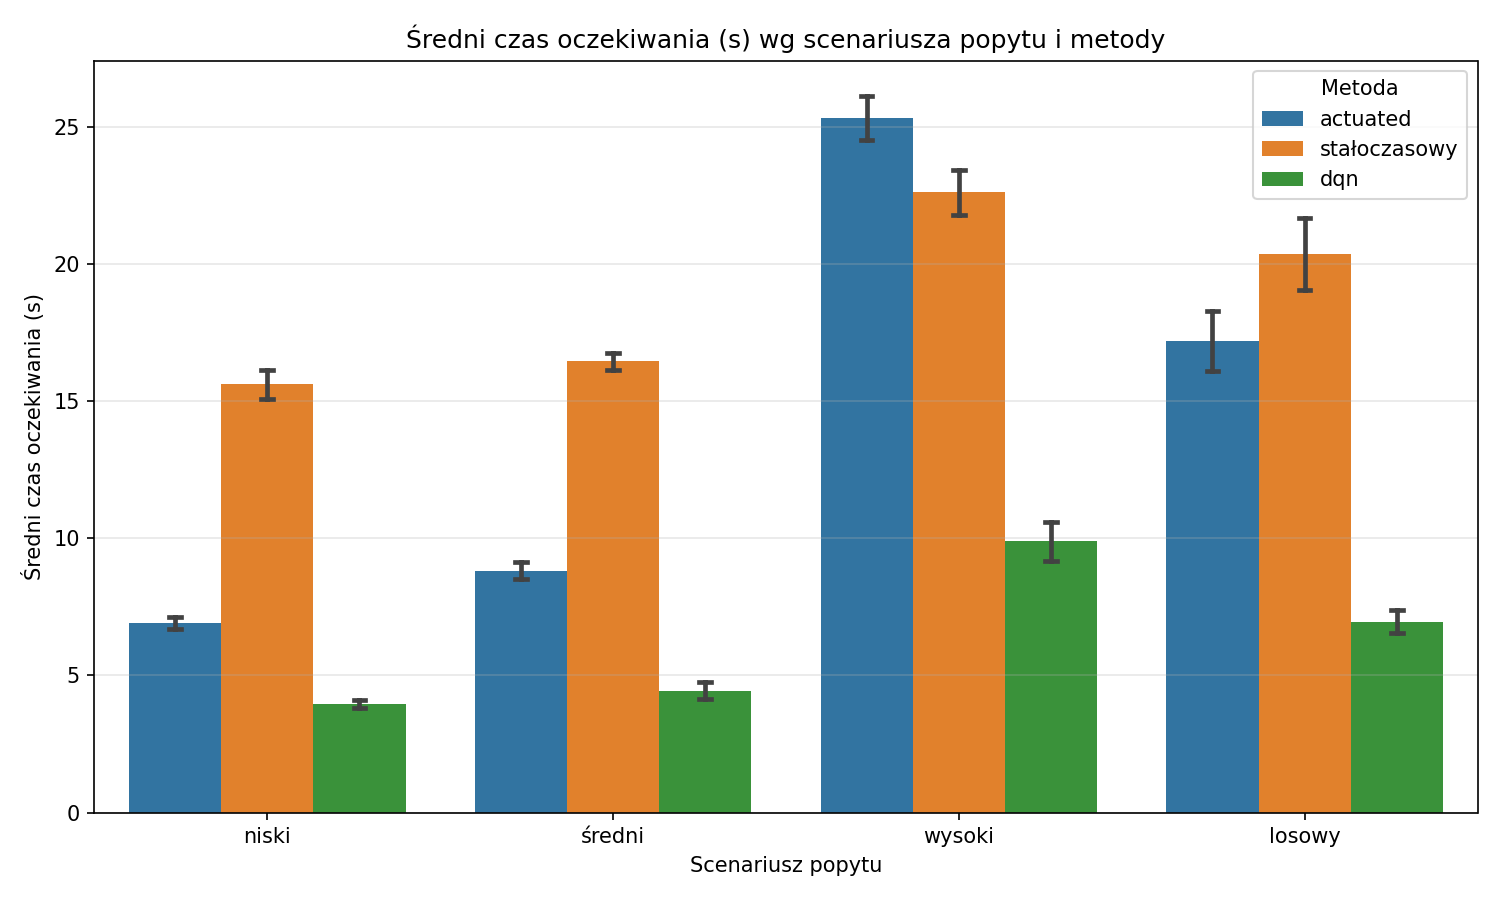
\includegraphics[width=0.8\linewidth]{results_bar_mean_waiting_simp.png}
    \caption{Średni czas oczekiwania według scenariusza natężenia oraz metody sterowania.}
    \label{fig:test-oczekiwanie}
\end{figure}

Uporządkowanie metod jest takie samo jak dla opóźnienia, jednak różnice względne są większe. Agent DQN skraca czas oczekiwania względem programu stałoczasowego o 32,4\% do 73,6\%, a względem programu akomodacyjnego o 3,5\% do 46,4\%. Największa różnica występuje ponownie w scenariuszu o wysokim natężeniu.

Metryka ta jest bezpośrednio powiązana z funkcją nagrody wykorzystaną podczas treningu, opisaną w podrozdziale~\ref{subsubsec:nagroda}, co należy uwzględnić przy interpretacji wyniku.

Uzupełniająco rejestrowano również wartości opisujące pojazdy obsłużone najgorzej. Kwantyl rzędu 0,95 czasu oczekiwania wynosi dla agenta DQN 19,20, 25,00, 78,41 oraz 59,45 w kolejnych scenariuszach. W ruchu lekkim i średnim jest on nieznacznie wyższy niż dla programu akomodacyjnego, wynoszącego tam 17,01 oraz 24,60, natomiast w ruchu wysokim i zmiennym wyraźnie niższy, wobec 201,21 oraz 83,76. Podobną zależność wykazuje maksymalny czas oczekiwania.

\subsubsection{Średnia długość kolejki}
\label{subsubsec:test-kolejka}

Wartości średniej długości kolejki zestawiono w tabeli~\ref{tab:test-kolejka}, a ich porównanie przedstawiono na rysunku~\ref{fig:test-kolejka}.

\begin{table}[!htbp] \centering
    \caption{Średnia długość kolejki na zbiorze testowym w pojazdach. W nawiasie odchylenie standardowe.}
    \label{tab:test-kolejka}
    \small
    \begin{tabular}{| l | r | r | r | r |} \hline
        Metoda & Lekki & Średni & Wysoki & Zmienny \\ \hline\hline
        stałoczasowa & 3,48 (0,13) & 7,37 (0,12) & 27,17 (1,40) & 12,37 (1,01) \\ \hline
        akomodacyjna & 1,13 (0,06) & 2,90 (0,15) & 25,88 (1,38) & \textbf{8,88} (0,91) \\ \hline
        \textbf{DQN} & \textbf{1,01} (0,07) & \textbf{2,83} (0,12) & \textbf{18,04} (4,33) & 9,55 (2,95) \\ \hline
    \end{tabular}
\end{table}

\begin{figure}[!htbp] \centering
    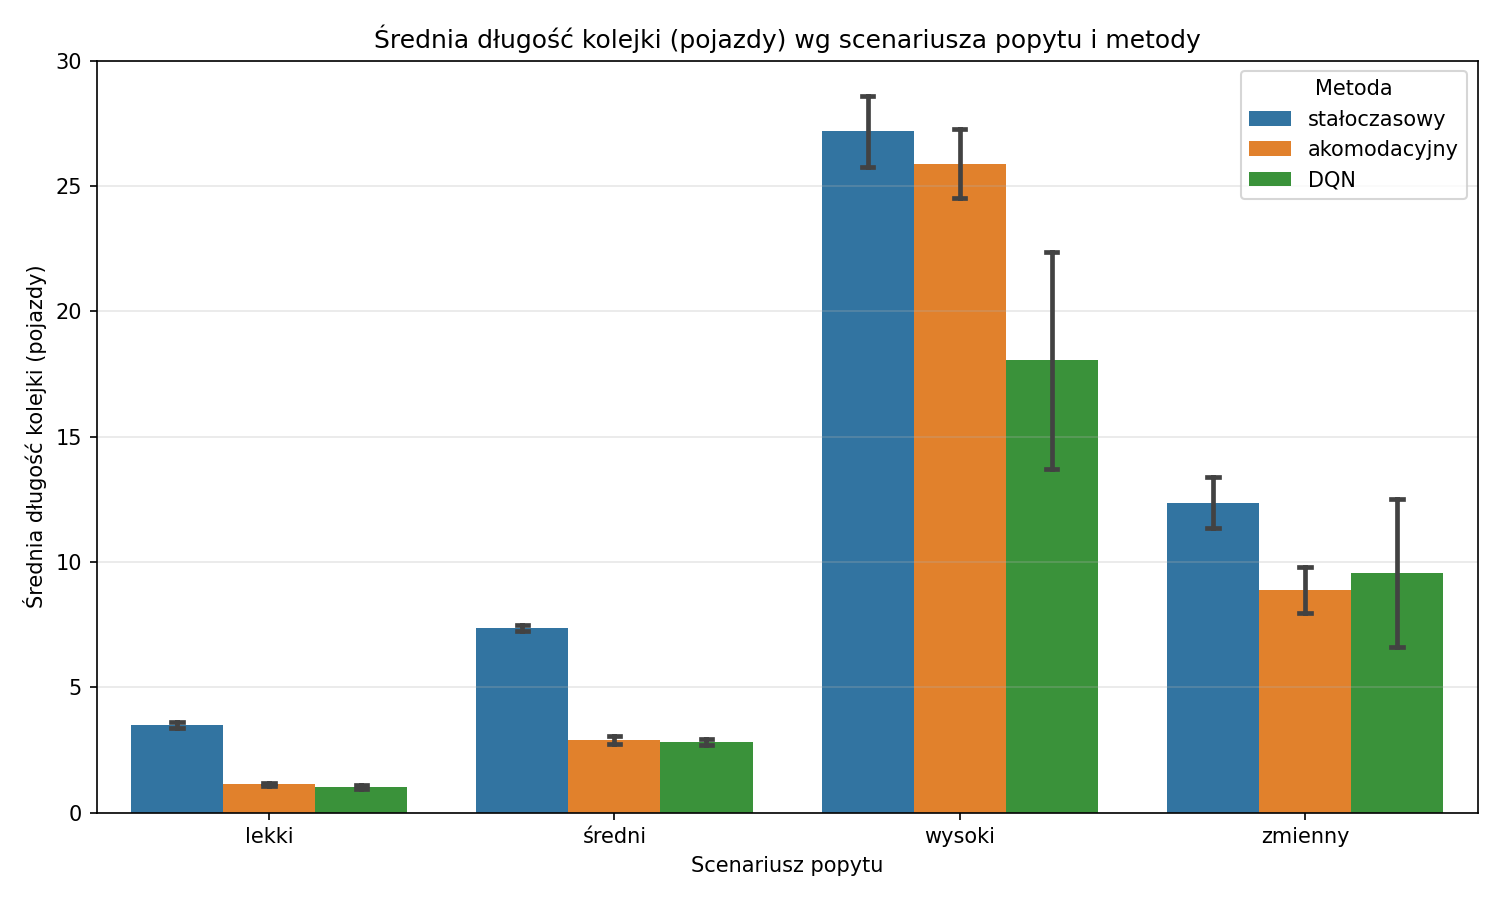
\includegraphics[width=0.8\linewidth]{results_bar_mean_queue_simp.png}
    \caption{Średnia długość kolejki według scenariusza natężenia oraz metody sterowania.}
    \label{fig:test-kolejka}
\end{figure}

Jest to jedyna metryka opisująca płynność ruchu, w której agent DQN nie osiąga najlepszego wyniku we wszystkich scenariuszach. W ruchu lekkim, średnim i wysokim uzyskuje wartości najniższe, natomiast w ruchu zmiennym wypada nieznacznie gorzej od programu akomodacyjnego, to jest 9,55 wobec 8,88, przy czym odchylenie standardowe wynosi tam 2,95 wobec 0,91.

Wynik w ruchu zmiennym jest jednocześnie metryką najsilniej obciążoną zjawiskiem opisanym w podrozdziale~\ref{subsubsec:przebieg-oceny-testowej}. Po pominięciu przebiegów przerwanych limitem czasu średnia długość kolejki agenta w tym scenariuszu wynosi 7,63, a w scenariuszu o wysokim natężeniu 19,96.

Uzupełniająco rejestrowano również długość kolejki w podziale na cztery wloty. Dla agenta DQN w scenariuszu o wysokim natężeniu wartości te mieszczą się w przedziale od 1,71 do 7,97 pojazdu, a więc stosunek największej do najmniejszej wynosi 4,7. Dla programu stałoczasowego przedział ten wynosi od 3,93 do 10,91, co odpowiada stosunkowi 2,8, a dla programu akomodacyjnego od 3,30 do 12,36, czyli 3,7. Rozkład obciążenia między wlotami jest zatem dla agenta bardziej nierównomierny, mimo niższej wartości sumarycznej.

\subsubsection{Przepustowość}
\label{subsubsec:test-przepustowosc}

Wartości przepustowości zestawiono w tabeli~\ref{tab:test-przepustowosc}, a ich porównanie przedstawiono na rysunku~\ref{fig:test-przepustowosc}.

\begin{table}[!htbp] \centering
    \caption{Przepustowość na zbiorze testowym w pojazdach na godzinę. W nawiasie odchylenie standardowe.}
    \label{tab:test-przepustowosc}
    \small
    \begin{tabular}{| l | r | r | r | r |} \hline
        Metoda & Lekki & Średni & Wysoki & Zmienny \\ \hline\hline
        stałoczasowa & 700,75 (4,54) & 1399,00 (7,70) & 2569,91 (75,56) & 1556,97 (24,82) \\ \hline
        akomodacyjna & 705,48 (4,03) & 1405,34 (3,06) & 2507,31 (119,38) & 1567,39 (35,73) \\ \hline
        \textbf{DQN} & \textbf{707,02} (4,47) & \textbf{1409,39} (2,83) & \textbf{2700,90} (65,04) & \textbf{1594,49} (38,04) \\ \hline
    \end{tabular}
\end{table}

\begin{figure}[!htbp] \centering
    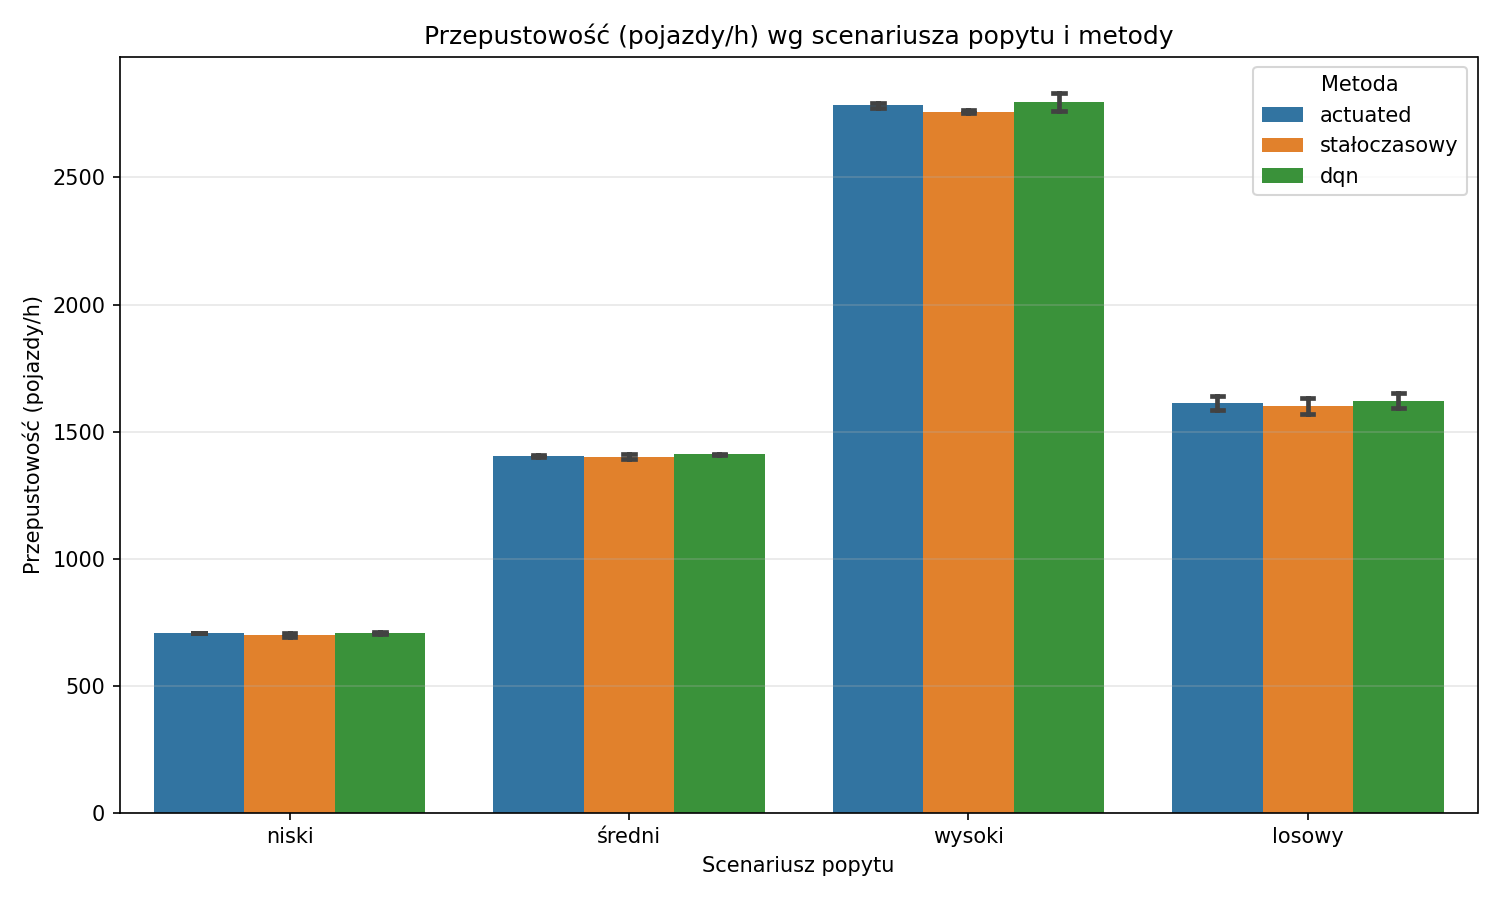
\includegraphics[width=0.8\linewidth]{results_bar_throughput_simp.png}
    \caption{Przepustowość według scenariusza natężenia oraz metody sterowania.}
    \label{fig:test-przepustowosc}
\end{figure}

W scenariuszach o lekkim i średnim natężeniu wszystkie trzy metody osiągają praktycznie identyczną przepustowość, różniącą się o mniej niż 1\%. Odpowiada to sytuacji, w której popyt jest niższy od możliwości skrzyżowania, więc metryka ta nie różnicuje metod.

Różnice pojawiają się w scenariuszu o wysokim natężeniu. Agent DQN obsługuje tam 2700,90 pojazdu na godzinę, czyli o 5,1\% więcej niż program stałoczasowy i o 7,7\% więcej niż akomodacyjny. W scenariuszu o zmiennym natężeniu przewaga jest mniejsza i wynosi 2,4\% oraz 1,7\%.

\subsubsection{Częstotliwość przełączeń}
\label{subsubsec:test-przelaczenia}

Wartości częstotliwości przełączeń zestawiono w tabeli~\ref{tab:test-przelaczenia}, a ich porównanie przedstawiono na rysunku~\ref{fig:test-przelaczenia}.

\begin{table}[!htbp] \centering
    \caption{Częstotliwość przełączeń na zbiorze testowym w przełączeniach na godzinę. W nawiasie odchylenie standardowe. Dla agenta DQN podano dodatkowo wartość wyznaczoną bez przebiegów przerwanych limitem czasu.}
    \label{tab:test-przelaczenia}
    \footnotesize
    \setlength{\tabcolsep}{5pt}
    \begin{tabular}{| l | r | r | r | r |} \hline
        Metoda & Lekki & Średni & Wysoki & Zmienny \\ \hline\hline
        stałoczasowa & 132,95 (0,38) & 132,90 (0,31) & 133,04 (0,32) & 132,78 (0,33) \\ \hline
        akomodacyjna & 405,63 (2,24) & 335,33 (8,14) & 133,13 (9,50) & 286,82 (6,24) \\ \hline
        DQN          & 272,00 (10,96) & 319,07 (5,04) & 232,85 (101,33) & 193,94 (127,03) \\ \hline
        DQN, bez przebiegów przerwanych & 272,00 & 319,07 & 278,10 & 286,69 \\ \hline
    \end{tabular}
\end{table}

\begin{figure}[!htbp] \centering
    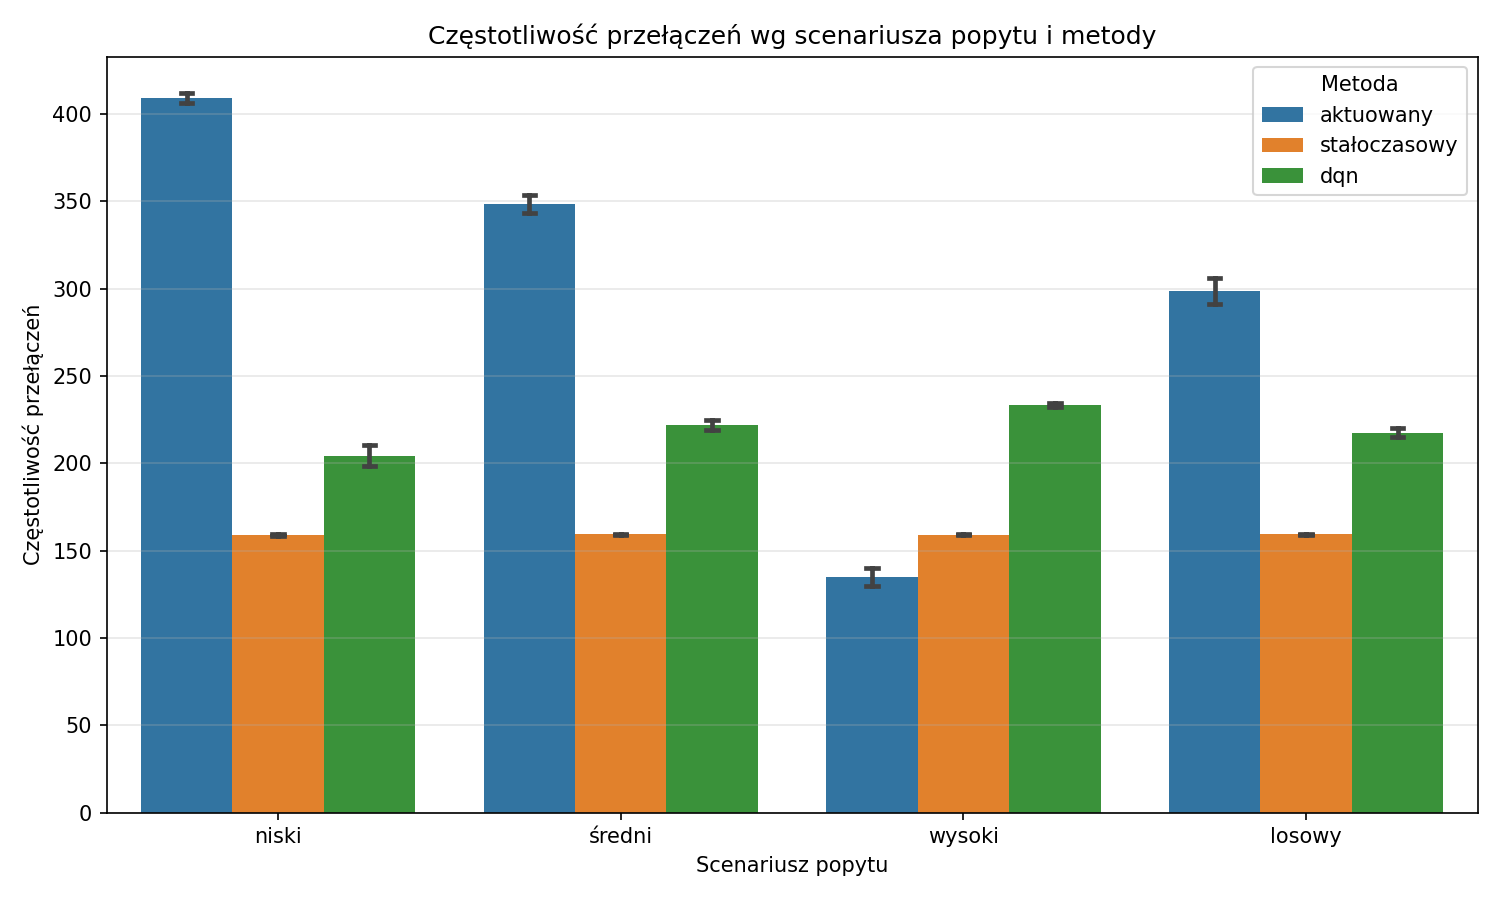
\includegraphics[width=0.8\linewidth]{results_bar_switching_freq_simp.png}
    \caption{Częstotliwość przełączeń według scenariusza natężenia oraz metody sterowania.}
    \label{fig:test-przelaczenia}
\end{figure}

Metryka ta wymaga ostrożnego odczytu, ponieważ wartości agenta DQN w scenariuszach o wysokim i zmiennym natężeniu obarczone są bardzo dużym odchyleniem standardowym, wynoszącym 101,33 oraz 127,03. Rozrzut ten nie wynika z różnej liczby przełączeń, lecz z różnej długości przebiegu. W przebiegach przerwanych limitem czasu liczba przełączeń pozostaje zbliżona do pozostałych, natomiast dzielona jest przez czas kilkukrotnie dłuższy. Po pominięciu tych przebiegów częstotliwość przełączeń agenta mieści się we wszystkich scenariuszach w przedziale od 272,00 do 319,07 i wykazuje niewielki rozrzut.

Po uwzględnieniu tej korekty obraz jest następujący. Program stałoczasowy przełącza sygnalizację ze stałą częstotliwością około 133 przełączeń na godzinę, niezależnie od scenariusza. Program akomodacyjny przełącza najczęściej w ruchu lekkim, gdzie osiąga 405,63, i coraz rzadziej wraz ze wzrostem natężenia, aż do 133,13 w ruchu wysokim. Agent DQN utrzymuje częstotliwość pośrednią, od 272,00 do 319,07, przy czym w ruchu lekkim przełącza rzadziej od programu akomodacyjnego, a w ruchu wysokim ponad dwukrotnie częściej.

Obie metody reagujące na ruch przełączają zatem sygnalizację częściej niż program stałoczasowy, jednak zależność tej częstotliwości od natężenia ruchu jest w ich przypadku odmienna.

\subsection{Ocena modelu kontrastowego}
\label{subsec:model-kontrastowy}

\subsubsection{Cel eksperymentu}
\label{subsubsec:cel-kontrastowy}

Wszystkie decyzje dotyczące konfiguracji podejmowano na podstawie zbioru walidacyjnego, przy założeniu, że wyniki walidacyjne są wskaźnikiem zdolności modelu do działania na danych wcześniej niewidzianych. Aby sprawdzić to założenie, na zbiorze testowym oceniono dodatkowo jeden model o najsłabszych wynikach walidacyjnych.

Wybrano wariant ze skróconą fazą eksploracji, oznaczony w tabeli~\ref{tab:strojenie} jako \texttt{explore1e-1}, którego średnie opóźnienie walidacyjne wynosiło 51,70 wobec 30,33 dla konfiguracji bazowej. Model ten określany jest dalej jako model kontrastowy. Nie stanowi on kolejnego kandydata wybieranego na podstawie wyników testowych, lecz element analizy wykonanej po zakończeniu procesu selekcji modelu końcowego.

\subsubsection{Wyniki}
\label{subsubsec:wyniki-kontrastowy}

Porównanie obu modeli przedstawiono w tabeli~\ref{tab:kontrastowy} oraz na rysunkach~\ref{fig:kontrastowy-opoznienie} i~\ref{fig:kontrastowy-kolejka}.

\begin{table}[!htbp] \centering
    \caption{Model końcowy i model kontrastowy na zbiorze testowym. W nawiasie odchylenie standardowe.}
    \label{tab:kontrastowy}
    \footnotesize
    \setlength{\tabcolsep}{4pt}
    \begin{tabular}{| l | l | r | r | r | r |} \hline
        Metryka & Model & Lekki & Średni & Wysoki & Zmienny \\ \hline\hline
        opóźnienie [s]      & końcowy     & 13,90 (0,58) & 17,79 (0,42) & 51,82 (6,95)   & 34,23 (5,36) \\ \hline
        opóźnienie [s]      & kontrastowy & 15,68 (0,79) & 18,38 (0,50) & 111,41 (5,35)  & 71,96 (18,99) \\ \hline
        kolejka [poj.]      & końcowy     & 1,01 (0,07)  & 2,83 (0,12)  & 18,04 (4,33)   & 9,55 (2,95) \\ \hline
        kolejka [poj.]      & kontrastowy & 1,27 (0,12)  & 3,05 (0,13)  & 51,14 (13,62)  & 36,40 (15,10) \\ \hline
        przepustowość [poj./h] & końcowy     & 707,02 (4,47) & 1409,39 (2,83) & 2700,90 (65,04) & 1594,49 (38,04) \\ \hline
        przepustowość [poj./h] & kontrastowy & 706,41 (4,65) & 1409,62 (2,65) & 2129,49 (62,92) & 1439,62 (28,33) \\ \hline
    \end{tabular}
\end{table}

\begin{figure}[!htbp] \centering
    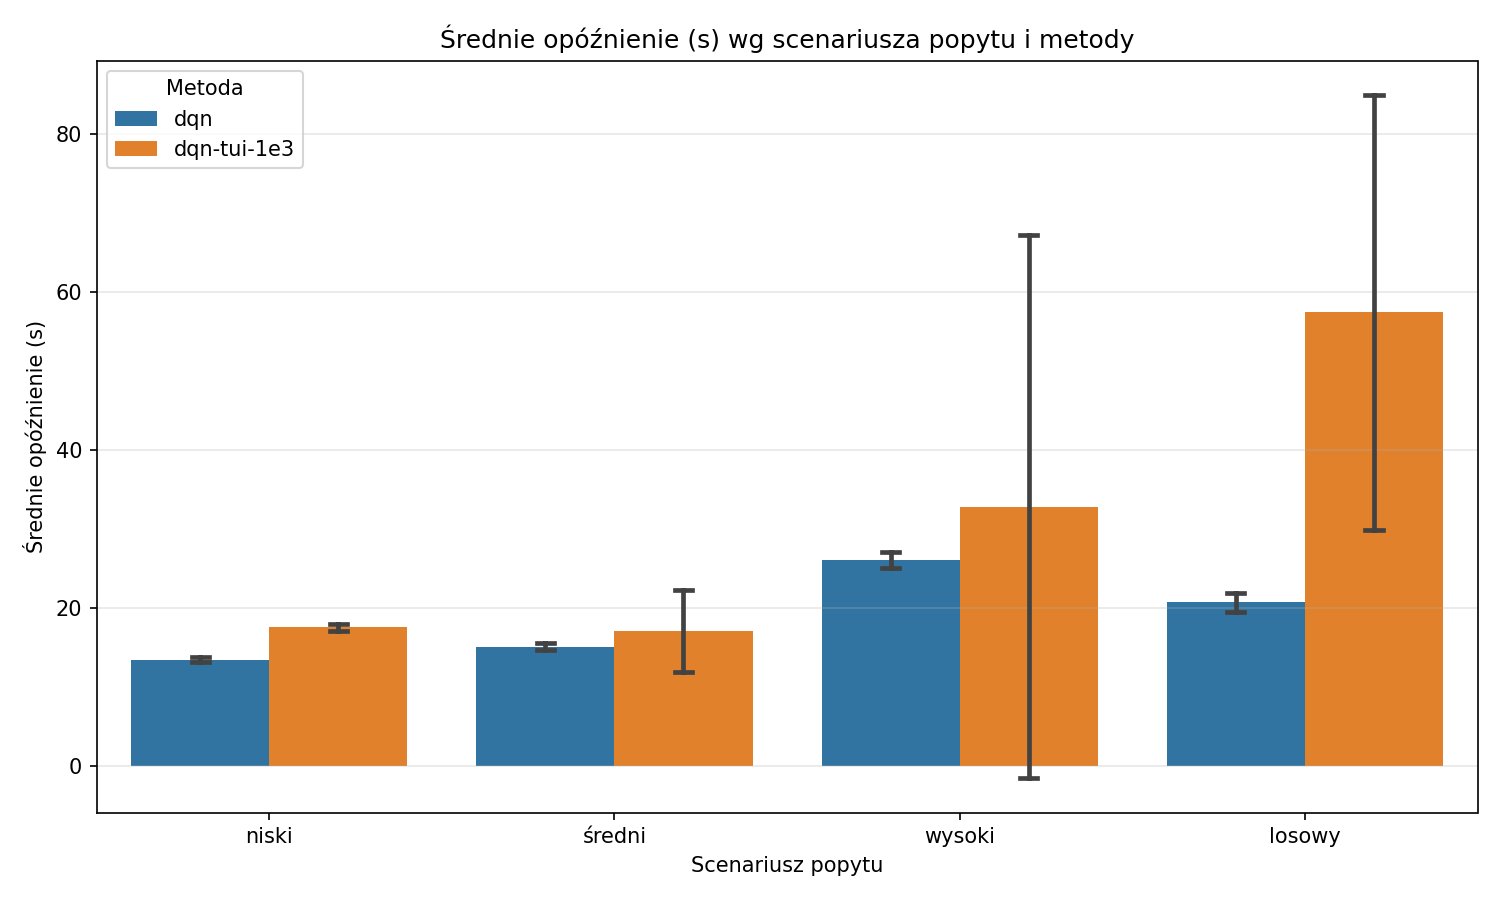
\includegraphics[width=0.8\linewidth]{results_bar_mean_delay_2.png}
    \caption{Średnie opóźnienie modelu końcowego i modelu kontrastowego.}
    \label{fig:kontrastowy-opoznienie}
\end{figure}

\begin{figure}[!htbp] \centering
    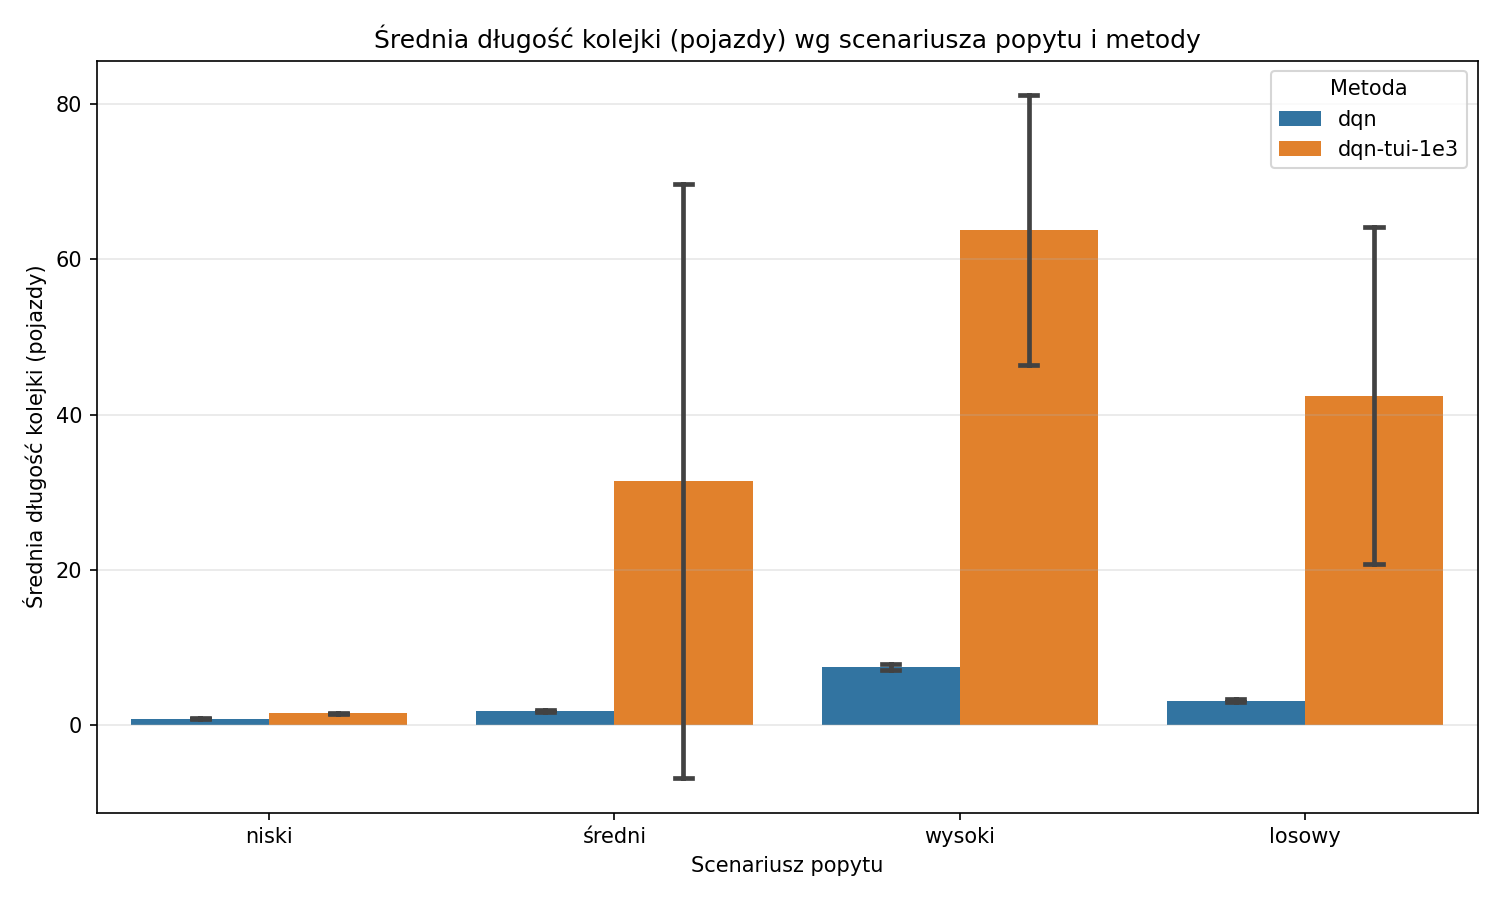
\includegraphics[width=0.8\linewidth]{results_bar_mean_queue_2.png}
    \caption{Średnia długość kolejki modelu końcowego i modelu kontrastowego.}
    \label{fig:kontrastowy-kolejka}
\end{figure}

Słaby wynik walidacyjny znalazł potwierdzenie na zbiorze testowym, jednak nie w jednakowym stopniu we wszystkich scenariuszach. W ruchu lekkim i średnim model kontrastowy jest gorszy od modelu końcowego jedynie o 12,8\% oraz 3,3\% pod względem opóźnienia, a jego wyniki pozostają lepsze od programu stałoczasowego i porównywalne z programem akomodacyjnym, którego opóźnienie wynosi tam 15,22 oraz 18,02. W tych warunkach model kontrastowy jest zatem sterownikiem poprawnym.

Różnica ujawnia się dopiero w scenariuszach trudniejszych. W ruchu wysokim opóźnienie rośnie o 115,0\%, do 111,41, a w ruchu zmiennym o 110,3\%, do 71,96. Model kontrastowy jest tam gorszy nie tylko od modelu końcowego, ale również od obu metod referencyjnych. Średnia długość kolejki rośnie odpowiednio o 183,5\% oraz 281,2\%, a przepustowość spada o 21,2\% oraz 9,7\%, co oznacza, że sterowanie nie jest w stanie obsłużyć zgłoszonego popytu.

Rozrzut wyników jest przy tym wyraźnie większy niż dla modelu końcowego. Odchylenie standardowe opóźnienia w ruchu zmiennym wynosi 18,99 wobec 5,36, a odchylenie średniej długości kolejki 15,10 wobec 2,95.

Model kontrastowy osiągnął limit czasu symulacji w dziesięciu z dwudziestu przebiegów, obejmujących wszystkie scenariusze o wysokim oraz wszystkie o zmiennym natężeniu. Skala zjawiska jest tu nieporównywalnie większa niż dla modelu końcowego: w jednym z przebiegów o wysokim natężeniu obsłużonych zostało 2371 z 2880 podróży, czyli 17,7\% pojazdów nie opuściło sieci. Z tego samego powodu częstotliwość przełączeń modelu kontrastowego spada w tych scenariuszach do wartości rzędu 51 przełączeń na godzinę, co jest artefaktem długości przebiegu, a nie oznaką rzadkiego przełączania.

Wyniki te pokazują, że słaba ocena walidacyjna przełożyła się na słabą generalizację, ale wyłącznie w scenariuszach o wysokim obciążeniu. Model, który w ruchu lekkim i średnim działałby akceptowalnie, przestaje działać skutecznie przy wysokim natężeniu ruchu. Obserwacja ta uzasadnia włączenie do zbioru walidacyjnego scenariusza reprezentującego warunki najtrudniejsze, ponieważ ocena oparta wyłącznie na scenariuszach o umiarkowanym obciążeniu nie ujawniłaby tej różnicy.

\subsection{Podsumowanie wyników}
\label{subsec:podsumowanie-wynikow}

Zbiorcze zestawienie wszystkich ocenionych metod przedstawiono w tabeli~\ref{tab:podsumowanie-wynikow}. Podano w niej średnie opóźnienie jako metrykę wiodącą oraz krótką charakterystykę zachowania każdej metody.

\begin{table}[!htbp] \centering
    \caption{Zbiorcze porównanie metod sterowania na zbiorze testowym. Wartości oznaczają średnie opóźnienie w sekundach na pojazd.}
    \label{tab:podsumowanie-wynikow}
    \footnotesize
    \begin{tabular}{| l | r | r | r | r | >{\raggedright\arraybackslash}p{4.4cm} |} \hline
        Metoda & Lekki & Średni & Wysoki & Zmienny & Charakterystyka \\ \hline\hline
        stałoczasowa & 28,00 & 30,91 & 65,45 & 48,25 & Przewidywalna, najgorsza przy niskim i średnim obciążeniu, stabilna przy wysokim natężeniu. \\ \hline
        akomodacyjna & 15,22 & 18,02 & 78,07 & 39,76 & Bardzo dobra przy niskim i średnim obciążeniu, najsłabsza z trzech głównych metod przy wysokim natężeniu. \\ \hline
        DQN & \textbf{13,90} & \textbf{17,79} & \textbf{51,82} & \textbf{34,23} & Najlepsza w każdym scenariuszu pod względem opóźnienia i czasu oczekiwania, kosztem większego rozrzutu wyników. \\ \hline
        DQN kontrastowy & 15,68 & 18,38 & 111,41 & 71,96 & Poprawna przy niskim i średnim obciążeniu, traci skuteczność przy wysokim natężeniu. \\ \hline
    \end{tabular}
\end{table}

Najważniejsze obserwacje ze zbioru testowego są następujące:
\begin{itemize}
    \item agent DQN uzyskał najniższe średnie opóźnienie oraz najniższy średni czas oczekiwania we wszystkich czterech scenariuszach natężenia ruchu;
    \item największa przewaga względem programu akomodacyjnego wystąpiła w scenariuszu o wysokim natężeniu, a najmniejsza w scenariuszu o średnim natężeniu, gdzie różnica opóźnienia wyniosła 1,3\%;
    \item średnia długość kolejki jest najniższa dla agenta w trzech z czterech scenariuszy, przy czym w scenariuszu o zmiennym natężeniu lepszy okazał się program akomodacyjny;
    \item przepustowość różnicuje metody wyłącznie w scenariuszu o wysokim natężeniu, gdzie agent obsłużył o 5,1\% oraz 7,7\% pojazdów więcej niż metody referencyjne;
    \item częstotliwość przełączeń agenta jest pośrednia między obiema metodami klasycznymi i zmienia się wraz z natężeniem ruchu inaczej niż w programie akomodacyjnym;
    \item żadna z metod klasycznych nie była lepsza we wszystkich scenariuszach, co potwierdza konieczność oceny na kilku poziomach obciążenia;
    \item rozrzut wyników agenta w scenariuszach o wysokim i zmiennym natężeniu jest porównywalny z rozrzutem programu akomodacyjnego i większy niż programu stałoczasowego;
    \item w trzech z dwudziestu przebiegów agenta niewielka grupa pojazdów nie opuściła sieci w zakładanym czasie, co nie wpłynęło na metryki wyznaczane z zakończonych podróży, lecz zniekształciło metryki normowane czasem trwania symulacji.
\end{itemize}

\clearpage
\section{Analiza wyników, ograniczenia i kierunki rozwoju}
\label{sec:analiza}
\clearpage
\section{Podsumowanie}
\label{sec:podsumowanie}

Celem pracy było sprawdzenie, czy agent wykorzystujący algorytm Deep Q-Network może skutecznie sterować sygnalizacją świetlną na pojedynczym skrzyżowaniu i osiągać lepsze rezultaty niż wybrane klasyczne metody sterowania. Badanie przeprowadzono w środowisku symulacyjnym na modelu skrzyżowania ulicy Belgradzkiej i alei Komisji Edukacji Narodowej. Zakres pracy dobrano tak, aby możliwe było przeprowadzenie kompletnego, kontrolowanego eksperymentu, obejmującego przygotowanie środowiska, trening, walidację oraz ocenę na odrębnym zbiorze testowym.

\subsection{Zrealizowane prace}
\label{subsec:podsumowanie-prace}

W ramach pracy przygotowano model skrzyżowania w symulatorze SUMO, obejmujący geometrię dróg, trzynaście pasów wlotowych, relacje skrętne oraz trzy fazy sygnalizacji. Zaimplementowano dwa punkty odniesienia: sterowanie stałoczasowe oraz sterowanie akomodacyjne typu \textit{gap-based}. Parametry obu metod wyznaczono na podstawie danych treningowych, a następnie zamrożono przed oceną modelu DQN.

Opracowano rozdzielne zbiory treningowy, walidacyjny i testowy, reprezentujące lekkie, średnie, wysokie oraz zmienne natężenie ruchu. Przygotowano dwa warianty danych treningowych, różniące się regularnością napływu pojazdów. Zbiór testowy obejmował dwadzieścia scenariuszy niewykorzystywanych podczas uczenia ani doboru konfiguracji.

Na podstawie biblioteki \texttt{sumo-rl} zbudowano własną warstwę integrującą SUMO z implementacją algorytmu DQN dostępną w bibliotece Stable-Baselines3. Dostosowano przebieg kroku środowiska, obsługę wielu plików tras oraz sposób zbierania metryk, dzięki czemu wszystkie metody oceniano według wspólnej procedury. Rejestrowano średnie opóźnienie, średni czas oczekiwania, długość kolejek, przepustowość i częstotliwość przełączeń sygnalizacji.

Proces uczenia obejmował ocenę kolejnych checkpointów, porównanie obu wariantów zbioru treningowego oraz sprawdzenie szesnastu wariantów konfiguracji hiperparametrów. Wybrane modele poddano dodatkowej walidacji na kilku ziarnach symulacji. Po zakończeniu tego etapu zamrożono model końcowy i oceniono go na tych samych scenariuszach testowych co metody referencyjne.

\subsection{Najważniejsze wyniki}
\label{subsec:podsumowanie-wyniki}

Modelem końcowym został checkpoint konfiguracji bazowej po 225\,000 kroków, wytrenowany na zbiorze o regularnym napływie pojazdów. Bardziej nieregularny zbiór treningowy nie poprawił wyników walidacyjnych, a żaden z szesnastu sprawdzonych wariantów hiperparametrów nie przewyższył konfiguracji bazowej na całym zbiorze walidacyjnym. Dalsze prowadzenie treningu do 300\,000 kroków również nie przyniosło poprawy, co potwierdziło znaczenie wyboru checkpointu na podstawie walidacji zamiast przyjmowania ostatniego zapisanego modelu.

Agent DQN uzyskał najniższe średnie opóźnienie i średni czas oczekiwania we wszystkich czterech grupach scenariuszy testowych. Średnie opóźnienie wyniosło odpowiednio 13,90~s dla ruchu lekkiego, 17,79~s dla średniego, 51,82~s dla wysokiego oraz 34,23~s dla zmiennego. Względem sterowania stałoczasowego oznacza to redukcję od 20,8\% do 50,4\%, natomiast względem sterowania akomodacyjnego od 1,3\% do 33,6\%. Największa przewaga nad metodą akomodacyjną wystąpiła przy wysokim natężeniu, a najmniejsza przy średnim, gdzie obie metody osiągnęły zbliżone rezultaty.

Przy wysokim natężeniu agent uzyskał również większą przepustowość niż obie metody referencyjne. Przewaga DQN była więc najbardziej widoczna w warunkach, w których sposób podziału czasu między fazy wpływał na zdolność obsłużenia popytu.

DQN nie był jednak najlepszy według każdej metryki. W scenariuszu zmiennym sterowanie akomodacyjne uzyskało mniejszą średnią długość kolejki, równą 8,88 pojazdu wobec 9,55 dla agenta. Metoda akomodacyjna osiągnęła także nieznacznie lepszy kwantyl rzędu 0,95 czasu oczekiwania przy lekkim i średnim ruchu. Program stałoczasowy przełączał sygnalizację znacznie rzadziej i działał bardziej przewidywalnie. W trzech z dwudziestu przebiegów modelu końcowego niewielka grupa pojazdów nie opuściła sieci przed limitem czasu, przy czym w każdym z tych przebiegów stanowiła mniej niż 1\% zgłoszonego popytu. Brak metryk tych pojazdów ogranicza siłę wniosków dotyczących przerwanych przebiegów i wskazuje aspekt wymagający dalszego doskonalenia.

\subsection{Odpowiedź na pytanie badawcze}
\label{subsec:odpowiedz-badawcza}

Na podstawie przeprowadzonego eksperymentu na pytanie badawcze można odpowiedzieć twierdząco: w przyjętych warunkach odpowiednio wytrenowany agent DQN sterował sygnalizacją skuteczniej niż badane sterowanie stałoczasowe i akomodacyjne pod względem średniego opóźnienia oraz średniego czasu oczekiwania. Przewaga wystąpiła we wszystkich grupach scenariuszy, chociaż jej skala zależała od natężenia ruchu. Przy średnim obciążeniu różnica względem sterowania akomodacyjnego była niewielka, natomiast przy wysokim natężeniu agent uzyskał wyraźnie lepsze wyniki także pod względem przepustowości.

Hipotezę badawczą uznano zatem za potwierdzoną warunkowo w zakresie badanego eksperymentu. Została ona potwierdzona dla opóźnienia i czasu oczekiwania oraz w większości scenariuszy dla długości kolejek. Wyjątek stanowił scenariusz zmienny, w którym podstawowy wynik kolejki był korzystniejszy dla sterowania akomodacyjnego. Rezultaty nie oznaczają, że DQN przewyższa każdą metodę klasyczną, w każdych warunkach i według każdego kryterium. Pokazują natomiast, że uczenie ze wzmocnieniem może doprowadzić do powstania skutecznej polityki sterowania, konkurencyjnej wobec starannie skonfigurowanych metod referencyjnych.

Zakres pracy świadomie ograniczono do pojedynczego skrzyżowania, syntetycznych scenariuszy i jednego głównego algorytmu RL. Wynik należy więc rozumieć jako potwierdzenie potencjału DQN w rozpatrywanym zadaniu, a nie jako ocenę wszystkich systemów sterowania ruchem ani gotowości rozwiązania do bezpośredniego wdrożenia. Dalsze badania powinny objąć kalibrację na danych pomiarowych, inne geometrie, więcej ziaren treningu, dodatkowych uczestników ruchu oraz pełną warstwę bezpieczeństwa.


%---------------
% Bibliografia
%---------------
\cleardoublepage % Zaczynamy od nieparzystej strony
\begingroup
\raggedright
\printbibliography
\endgroup
\clearpage

% Wykaz symboli i skrótów.
% Pamiętaj, żeby posortować symbole alfabetycznie
% we własnym zakresie. Makro \acronymlist
% generuje właściwy tytuł sekcji, w zależności od języka.
% Makro \acronym dodaje skrót/symbol do listy,
% zapewniając podstawowe formatowanie.
\acronymlist
% \acronym{AE}{Autoenkoder}
% ....
\clearpage
%--------------------------------------
% Spisy: rysunków, tabel, załączników
%--------------------------------------
\pagestyle{plain}
\listoffigurestoc    % Spis rysunków.
\clearpage      % vertical space
\listoftablestoc     % Spis tabel.
\end{document} % Dobranoc.
